% This LaTeX document needs to be compiled with XeLaTeX.
\documentclass[10pt]{article}
\usepackage[utf8]{inputenc}
\usepackage{graphicx}
\usepackage[export]{adjustbox}
\graphicspath{ {./images/} }
\usepackage{amsmath}
\usepackage{amsfonts}
\usepackage{amssymb}
\usepackage[version=4]{mhchem}
\usepackage{stmaryrd}
\usepackage{hyperref}
\hypersetup{colorlinks=true, linkcolor=blue, filecolor=magenta, urlcolor=cyan,}
\urlstyle{same}
\usepackage[fallback]{xeCJK}
\usepackage{polyglossia}
\usepackage{fontspec}
\usepackage{newunicodechar}
\setCJKmainfont{Noto Serif CJK SC}

\setmainlanguage{english}
\setmainfont{CMU Serif}

%New command to display footnote whose markers will always be hidden
\let\svthefootnote\thefootnote
\newcommand\blfootnotetext[1]{%
  \let\thefootnote\relax\footnote{#1}%
  \addtocounter{footnote}{-1}%
  \let\thefootnote\svthefootnote%
}

%Overriding the \footnotetext command to hide the marker if its value is `0`
\let\svfootnotetext\footnotetext
\renewcommand\footnotetext[2][?]{%
  \if\relax#1\relax%
    \ifnum\value{footnote}=0\blfootnotetext{#2}\else\svfootnotetext{#2}\fi%
  \else%
    \if?#1\ifnum\value{footnote}=0\blfootnotetext{#2}\else\svfootnotetext{#2}\fi%
    \else\svfootnotetext[#1]{#2}\fi%
  \fi
}

\newunicodechar{×}{\ifmmode\times\else{$\times$}\fi}

\begin{document}
数学奥林匹克小丛书第二版\\

\includegraphics[max width=\textwidth, center]{2024_10_30_bd799899fef40368a068g-001}

初中卷\\

\includegraphics[max width=\textwidth, center]{2024_10_30_bd799899fef40368a068g-001(1)}

因式分解技巧\\
单 墫 著

数学奥林匹克小丛书\\
第二版\\
初中卷\\
1\\

\includegraphics[max width=\textwidth, center]{2024_10_30_bd799899fef40368a068g-002(1)}\\

\includegraphics[max width=\textwidth, center]{2024_10_30_bd799899fef40368a068g-002}

\section*{因式分解技巧}
单 墫 著

铂华东师范大学出版社

\section*{数学奥林匹克小丛书(第二版)编委会}
冯志刚 第53届IMO中国队副领队、上海中学特级教师\\
葛 军 博士、中国数学奥林匹克高级教练、南京师范大学副教授\\
江苏省中学数学教学研究会副理事长\\
冷岗松 国家集训队教练、上海大学教授、博士生导师\\
李胜宏 第44届IMO中国队领队、浙江大学教授、博士生导师\\
李伟固 中国数学奥林匹克委员会委员、国家集训队教练\\
北京大学教授、博士生导师\\
刘诗雄 华南师范大学中山附属中学校长、中学数学特级教师\\
倪 明 华东师范大学出版社教辅分社社长、编审\\
单 墫 第30、31届 1 MO 中国队领队、南京师范大学教授、博士生导师\\
吴建平 中国数学会普及工作委员会主任、中国数学奥林匹克委员会副主席\\
熊 斌 第46、49、51、52、53届IMO中国队领队\\
中国数学奥林匹克委员会委员、华东师范大学教授、博士生导师\\
余红兵 中国数学奥林匹克委员会委员、国家集训队教练苏州大学教授、博士生导师\\
朱华伟 中国教育数学学会常务副理事长、国家集训队教练\\
广州大学软件所所长、研究员

\section*{图书在版编目(CIP)数据}
数学奥林匹克小丛书. 初中卷. 因式分解技巧/单墫著.\\
-2 版. 一上海:华东师范大学出版社,2011. 12\\
ISBN 978-7-5617-9213-1\\
I. (1) 数… II. (1)单… III. (1)中学数学课一初中一教学参考资料 IV. (1)G634.603

中国版本图书馆 CIP 数据核字(2011)第282995号

数学奥林匹克小丛书(第二版) $\cdot$ 初中卷\\
因式分解技巧(第二版)

\begin{center}
\begin{tabular}{|c|c|}
\hline
著 者 & 单 墫 \\
\hline
总策 划 & 倪 明 \\
\hline
项目编辑 & 孔令志 \\
\hline
审读编辑 & 程丽明 \\
\hline
装帧设计 & 高 山 \\
\hline
责任发行 & 郑海兰 \\
\hline
出版发行 & 华东师范大学出版社 \\
\hline
社 址 & 上海市中山北路 3663 号 邮编 200062 \\
\hline
网 址 & www. ecnupress.com.cn \\
\hline
电 话 & 021-60821666 行政传真 021-62572105 \\
\hline
客服电话 & 021-62865537 门市(邮购) 电话 021-62869887 \\
\hline
地 址 & 上海市中山北路 3663 号华东师范大学校内先锋路口 \\
\hline
网 店 & http://hdsdcbs. tmall.com \\
\hline
印刷 者 & 常熟高专印刷有限公司 \\
\hline
开 本 & 787×1092 16 开 \\
\hline
插 页 & 1 \\
\hline
印 张 & 6.5 \\
\hline
字 数 & 110 千字 \\
\hline
版 次 & 2012年7月第二版 \\
\hline
印 次 & 2012年7月第一次 \\
\hline
印 数 & 1-13000 \\
\hline
书 号 & ISBN 978-7-5617-9213-1/G G 5510 \\
\hline
定 价 & 14.00 元 \\
\hline
出版 人 & 朱杰人 \\
\hline
\end{tabular}
\end{center}

\section*{心}
\begin{center}
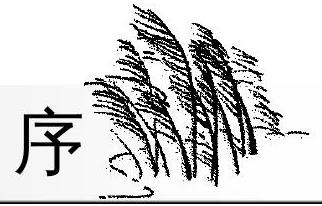
\includegraphics[max width=\textwidth]{2024_10_30_bd799899fef40368a068g-005}
\end{center}

数学竞赛像其他竞赛活动一样,是青少年学生的一种智力竞赛。在类似的以基础科学为竞赛内容的智力竞赛活动中,数学竞赛的历史最悠久、国际性强,影响也最大。我国于1956年开始举行数学竞赛,当时最有威望的著名数学家华罗庚、苏步青、江泽涵等都积极参加领导和组织竞赛活动,并组织出版了一系列青少年数学读物,激励了一大批青年学生立志从事科学事业。我国于1986年起参加国际数学奥林匹克,多次获得团体总分第一,并于1990年在北京成功地举办了第 31 届国际数学奥林匹克,这标志着我国数学竞赛水平在国际上居领先地位,为各国科学家与教育家所瞩目。

我国数学竞赛活动表明,凡是开展好的地区和单位,都能大大激发学生的学习数学的兴趣,有利于培养创造性思维,提高学生的学习效率。这项竞赛活动,将健康的竞争机制引进数学教学过程中,有利于选拔人才。由数学竞赛选拔的优胜者,既有踏实广泛的数学基础,又有刻苦钻研、科学的学习方法,其中的不少青年学生将来会成为出色的科学工作者。在美国,数学竞赛的优胜者中后来成名如米尔诺(J. W. Milnor)、芒福德(D. B. Mumford)、奎伦 (D. Quillen)等都是菲尔兹数学奖的获得者;在波兰,著名数论专家辛哲尔 (A. Schinzel)学生时代是一位数学竞赛优胜者;在匈牙利,著名数学家费叶尔 (L. Fejér)、里斯(M. Riesz)、舍贵(G. Szegö)、哈尔(A. Haar)、拉多 (T. Radó)等都曾是数学竞赛获奖者。匈牙利是开展数学竞赛活动最早的国家,产生了同它的人口不成比例的许多大数学家!

在开展数学竞赛的活动同时,各学校能加强联系,彼此交流数学教学经验,从这种意义上来说,数学竞赛可能成为数学课程改革的"催化剂",成为培养优秀人才的有力措施。

不过,应当注意在数学竞赛活动中,注意普及与提高相结合,而且要以普及为主,使竞赛具有广泛的群众基础,否则难以持久。

当然,现在有些人过于关注数学竞赛的成绩,组织和参与都具有很强的功利目的,过分扩大数学竞赛的作用,这些都是不正确的,违背了开展数学竞赛活动的本意。这些缺点有其深层次的社会原因,需要逐步加以克服,不必因

\section*{001}
为有某些缺点,就否定这项活动。\\
我十分高兴看到这套《数学奥林匹克小丛书》的正式出版。这套书,规模大、专题细。据我所知,这样的丛书还不多见。这套书不仅对数学竞赛中出现的常用方法作了阐述,而且对竞赛题作了精到的分析解答,不少出自作者自己的研究所得, 是一套很好的数学竞赛专题教程, 也是中小学生和教师的参考书。

这套小丛书的作者都是数学竞赛教学和研究人员,不少是国家集训队的教练和国家队的领队。他们为我国开展数学竞赛的活动和我国学生在 IMO 上取得成绩、为国争光作出了贡献,为这套书尽早面世付出了艰辛的劳动。华东师大出版社在出版《奥数教程》和《走向 IMO》等竞赛图书基础上,策划组织了这套丛书,花了不少心血。我非常感谢作者们和编辑们在这方面所做的工作,并衷心祝愿我国的数学竞赛活动开展得越来越好。

\section*{五元}
\footnotetext{王元,著名数学家,中国科学院院士,曾任中国数学会理事长、中国数学奥林匹克委员会主席.
}
0 什么是因式分解 ..... 001\\
1 提公因式 ..... 002\\
1.1 一次提净 ..... 002\\
1.2 视"多"为一 ..... 003\\
1.3 切勿漏 1 ..... 003\\
1.4 注意符号 ..... 004\\
1.5 仔细观察 ..... 004\\
1.6 化"分"为整 ..... 005\\
习题 1 ..... 006\\
2 应用公式 ..... 007\\
2.1 平方差 ..... 007\\
2.2 立方和与立方差 ..... 008\\
2.3 完全平方 ..... 008\\
2.4 完全立方 ..... 009\\
2.5 问一知三 ..... 010\\
2. $6 \quad 2^{1984}+1$ 不是质数 ..... 011\\
习题 2 ..... 012\\
3 分组分解 ..... 013\\
3.1 三步曲 ..... 013\\
3.2 殊途同归 ..... 013\\
3.3 平均分配 ..... 014\\
3.4 瞄准公式 ..... 015\\
3.5 从零开始 ..... 015\\
习题 3 ..... 017\\
4 拆项与添项 ..... 018\\
4.1 拆开中项 ..... 018\\
4.2 皆大欢喜 ..... 018\\
4.3 旧事重提 ..... 019\\
4.4 无中生有 ..... 019\\
4.5 配成平方 ..... 020\\
习题 4 ..... 021\\
5 十字相乘 ..... 022\\
5.1 知己知彼 ..... 022\\
5.2 熟能生巧 ..... 024\\
5.3 再进一步 ..... 025\\
5.4 二次齐次式 ..... 026\\
5.5 系数和为零 ..... 027\\
习题 5 ..... 028\\
6 二元二次式的分解 ..... 029\\
6.1 欲擒故纵 ..... 029\\
6.2 三元齐次 ..... 031\\
6.3 项数不全 ..... 032\\
6. 4 能否分解 ..... 032\\
习题 6 ..... 034\\
7 综合运用 ..... 035\\
7.1 善于换元 ..... 035\\
7.2 主次分清 ..... 037\\
7.3 一题两解 ..... 038\\
7.4 展开处理 ..... 039\\
7.5 巧运匠心 ..... 040\\
习题 7 ..... 042\\
8 多项式的一次因式 ..... 044\\
8.1 余数定理 ..... 044\\
8. 2 有理根的求法 ..... 045\\
8.3 首1多项式 ..... 047\\
8. 4 字母系数 ..... 049\\
习题 8 ..... 050\\
9 待定系数法 ..... 051\\
9.1 二次因式 ..... 051\\
9.2 既约的情况 ..... 054\\
习题 9 ..... 055\\
10 轮换式与对称式 ..... 056\\
10.1 典型方法 ..... 056\\
10.2 齐次与非齐次 ..... 059\\
10. $3 a^{3}+b^{3}+c^{3}-3 a b c$ ..... 061\\
10.4 焉用牛刀 ..... 062\\
10.5 整除问题 ..... 063\\
10.6 原来是零 ..... 065\\
10.7 四元多项式 ..... 067\\
习题 10 ..... 068\\
11 实数集与复数集内的分解 ..... 071\\
11.1 求根公式 ..... 071\\
11.2 代数基本定理 ..... 073\\
11.3 单位根 ..... 074\\
11.4 攻玉之石 ..... 076\\
习题 11 ..... 079\\
12 既约多项式 ..... 080\\
12.1 艾氏判别法 ..... 080\\
12.2 奇与偶 ..... 081\\
12.3 分圆多项式 ..... 083\\
12.4 绝对不可约 ..... 085\\
习题 12 ..... 085\\
习题答案 ..... 087

\section*{华东师大精品奥数图书}
\section*{学奥数,这里总有一本适合你}
"奥数"入门篇——《课本到奥数》(1-9 年级)本书或许不适合你,如果你\\
A. 每次考试都能超过 95 分-so easy!\\
B. 考试很少能超过 80 分一so difficult!\\
C. 不认为自己能学好数学一一Attitude first!读者对象:数学成绩班级前 $5 \%-30 \%$ 的优等生\\
"奥数"智优篇——《优等生数学》(1-9 年级)\\
如果说"奥数"是提供给 $4 \%$ 的优等生,\\
那么《优等生数学》提供给 $20 \%$ 的优等生。\\
如果你已经是优等生,不妨一读;\\
如果你想成为优等生,不能不读!\\
读者对象:数学成绩班级前 $20 \%$ 的优等生\\
"奥数"辅导篇——《奥数教程》、《学习手册》、《能力测试》

\begin{itemize}
  \item 第十届全国教育图书展优秀畅销图书
  \item 国家集训队教练执笔联合编写
  \item 在香港出版繁体字版和网络版
  \item 2010年最新修订,三本配套使用,效果更佳
\end{itemize}

读者对象:数学成绩班级前 $10 \%$ 的优等生、竞赛教练员\\
"奥数"题库篇——《多功能题典》初中、高中数学竞赛

\begin{itemize}
  \item 题量大、内容全、解法精
  \item 分类细:按照章节、难度、题型、方法等维度分类
  \item 配有网络检索功能 \href{http://tidian}{http://tidian}. ecnupress. com. cn读者对象:成绩优秀的中学生、竞赛教练员、数学爱好者\\
"奥数"课外阅读篇——《单墫老师教你学数学》 7 种\\
当读书不只是为了考试\\
你才会真正爱上数学\\
单墫老师妮娓道来\\
与你分享他所理解的数学之美\\
读者对象:初高中学生,数学教师,数学爱好者\\
"奥数"域外篇——《全俄中学生数学奥林匹克(1993-2006)》\\
俄罗斯是世界上开展数学活动最早、最广泛、也是影响最大的国家之一。俄罗斯是世界上竞赛试题的最大生产国,不仅产量高,而且质量好,其中最出色的当数组合题。
\end{itemize}

本书收录 1993-2006年俄罗斯 9-11年级数学奥林匹克第四轮(联邦区域竞赛)和第五轮(全俄决赛)竞赛的所有试题和解答。

读者对象:参加数学竞赛的中学生、竞赛教练员、数学爱好者\\
"奥数"高中预赛篇——《高中数学联赛备考手册(预赛试题集锦)》

\begin{itemize}
  \item 从2009年起,每年出版一册
  \item 收录了当年各省市预赛试题和优秀解答(约 20 份)
  \item 试题在遵循现行教学大纲, 体现新课标精神的同时, 在方法的要求上有所提高
  \item 命题人员大多同时兼任各省市高考命题工作,试题对高考有一定的指导作用\\
读者对象:参加预赛和联赛的高中生、竞赛教练员、高中教师\\
"奥数"联赛冲刺篇——《初(高)中数学联赛考前辅导》
  \item 选题经典且贴近高中联赛
  \item 知识上查漏补缺, 能力上全面提升
  \item 全新模拟题让你提前感受考场氛围
\end{itemize}

读者对象:参加联赛的高中生、竞赛教练员、高中教师\\
"奥数"IMO 终极篇——《走向 IMO:数学奥林匹克试题集锦》

\begin{itemize}
  \item 从 2003 年起,每年出版一册
  \item 以国家集训队测试题和国家队训练题为主
  \item 收集了国内主要竞赛:全国联赛、联赛加试、冬令营、女子数学奥林匹克、西部数学奥林匹克、东南地区数学奥林匹克
  \item 附有美国、俄罗斯、罗马尼亚和国际数学奥林匹克
\end{itemize}

读者对象:参加联赛、冬令营等赛事的高中生、竞赛教练员、数学爱好者\\
更多图书信息及免费资料请登录:\\
\href{http://www}{http://www}. hdsdjf. com/downloadfileinfor. aspx? classid=69

在小学里, 我们学过整数的因数分解. 由乘法, 得

\begin{align*}
3 \times 4=12
\end{align*}

反过来, 12 可以分解: $12=3 \times 4$.\\
当然, 4 还可以继续分解为 $2 \times 2$ 。于是得

\begin{align*}
12=3 \times 2 \times 2
\end{align*}

这时 12 已经分解成质因数的乘积了。\\
同样地, 由整式乘法, 得

\begin{align*}
(1+2 x)\left(1-x^{2}\right)=1+2 x-x^{2}-2 x^{3}
\end{align*}

反过来, $1+2 x-x^{2}-2 x^{3}$ 可以分解为两个因式 $1+2 x$ 与 $1-x^{2}$ 的乘积,即

\begin{align*}
1+2 x-x^{2}-2 x^{3}=(1+2 x)\left(1-x^{2}\right)
\end{align*}

$1-x^{2}$ 还可以继续分解为 $(1+x)(1-x)$. 于是

\begin{align*}
1+2 x-x^{2}-2 x^{3}=(1+2 x)(1+x)(1-x)
\end{align*}

这里 $x$ 的一次多项式 $1+2 x 、 1+x 、 1-x$ 都不能继续分解,它们是不可约多项式,也就是既约多项式。 所以, $1+2 x-x^{2}-2 x^{3}$ 已经分解成质因式的乘积了。

把一个整式写成几个整式的乘积,称为因式分解,每一个乘式称为积的因式。

在因式分解中,通常要求各个乘式(因式)都是既约多项式,这样的因式称为质因式。

因式分解的方法,我们将逐一介绍。

学过因式分解的人爱说: "一提、二代、三分组,"\\
"提"是指"提取公因式". 在因式分解时, 首先应当想到的是有没有公因式可提。

几个整式都含有的因式称为它们的公因式.\\
例如 $m a 、 m b 、-m c$ 都含有因式 $m, m$ 就是它们的公因式。\\
由乘法分配律,我们知道

因此

\begin{align*}
\begin{align*}
& m(a+b-c)=m a+m b-m c, \\
& m a+m b-m c=m(a+b-c) .
\end{align*} \tag{1}
\end{align*}

这表明 (1) 式左边三项的公因式 $m$ 可以提取出来,作为整式 $m a+m b-$ $m c$ 的因式. $m a+m b-m c$ 的另一个因式 $a+b-c$ 仍由三项组成, 每一项等于 $m a+m b-m c$ 中对应的项除以公因式 $m$ :

\begin{align*}
a=m a \div m, b=m b \div m, c=m c \div m
\end{align*}

\section*{1.1 一次提净}
例1 分解因式: $12 a^{2} x^{3}+6 a b x^{2} y-15 a c x^{2}$ 。\\
解 $12 a^{2} x^{3}+6 a b x^{2} y-15 a c x^{2}$ 由

\begin{align*}
12 a^{2} x^{3}, 6 a b x^{2} y,-15 a c x^{2}
\end{align*}

这三项组成,它们的数系数 $12 、 6 、-15$ 的最大公约数是 3 ,各项都含有因式 $a$和 $x^{2}$, 所以 $3 a x^{2}$ 是上述三项的公因式, 可以提取出来作为 $12 a^{2} x^{3}+6 a b x^{2} y-$ $15 a c x^{2}$ 的因式, 即有

\begin{align*}
\begin{aligned}
& 12 a^{2} x^{3}+6 a b x^{2} y-15 a c x^{2} \\
= & 3 a x^{2}(4 a x+2 b y-5 c) .
\end{aligned}
\end{align*}

在例 1 中, 如果只将因式 $3 a$ 或 $3 a x$ 提出, 那么留下的式子仍有公因式可

以提取, 这增添了麻烦, 不如一次提净为好. 因此, 应当先检查数系数, 然后再一个个字母逐一检查,将各项的公因式提出来,使留下的式子没有公因式可以直接提取。

还需注意原式如果由三项组成,那么提取公因式后留下的式子仍由三项组成. 在例1 中,这三项分别为 $12 a^{2} x^{3} 、 6 a b x^{2} y 、-15 a c x^{2}$ 除以公因式 $3 a x^{2}$ 所得的商. 初学的同学为了防止产生错误,可以采取两点措施:

\begin{enumerate}
  \item 在提公因式前, 先将原式的三项都写成公因式 $3 a x^{2}$ 与另一个式子的积,然后再提取公因式,即
\end{enumerate}

\begin{align*}
\begin{aligned}
& 12 a^{2} x^{3}+6 a b x^{2} y-15 a c x^{2} \\
= & 3 a x^{2} \cdot 4 a x+3 a x^{2} \cdot 2 b y+3 a x^{2} \cdot(-5 c) \\
= & 3 a x^{2} \cdot(4 a x+2 b y-5 c) .
\end{aligned}
\end{align*}

在熟练之后应当省去中间过程,直接写出结果。\\
2. 用乘法分配律进行验算. 由乘法得出

\begin{align*}
\begin{aligned}
& 3 a x^{2}(4 a x+2 b y-5 c) \\
= & 12 a^{2} x^{3}+6 a b x^{2} y-15 a c x^{2} .
\end{aligned}
\end{align*}

\section*{1.2 视"多"为一}
例2 分解因式: $2 a^{2} b(x+y)^{2}(b+c)-6 a^{3} b^{3}(x+y)(b+c)^{2}$ 。\\
解 原式由

\begin{align*}
2 a^{2} b(x+y)^{2}(b+c) 、-6 a^{3} b^{3}(x+y)(b+c)^{2}
\end{align*}

这两项组成。它们的数系数的最大公约数是 2 , 两项都含有因式 $a^{2}$ 和 $b$, 而且都含有因式 $x+y$ 与 $b+c$, 因此 $2 a^{2} b(x+y)(b+c)$ 是它们的公因式. 于是有

\begin{align*}
\begin{aligned}
& 2 a^{2} b(x+y)^{2}(b+c)-6 a^{3} b^{3}(x+y)(b+c)^{2} \\
= & 2 a^{2} b(x+y)(b+c) \cdot(x+y)-2 a^{2} b(x+y)(b+c) \cdot 3 a b^{2}(b+c) \\
= & 2 a^{2} b(x+y)(b+c)\left[(x+y)-3 a b^{2}(b+c)\right] \\
= & 2 a^{2} b(x+y)(b+c)\left(x+y-3 a b^{3}-3 a b^{2} c\right) .
\end{aligned}
\end{align*}

在本例中,我们把多项式 $x+y 、 b+c$ 分别整个看成是一个字母,这种观点在因式分解时是很有用的。

\section*{1.3 切勿漏 1}
例3 分解因式: $(2 x+y)^{3}-(2 x+y)^{2}+(2 x+y)$.

解 我们把多项式 $2 x+y$ 看成是一个字母,因此原式由

\begin{align*}
(2 x+y)^{3},-(2 x+y)^{2}, 2 x+y
\end{align*}

这三项组成, $2 x+y$ 是这三项的公因式,于是

\begin{align*}
\begin{aligned}
& (2 x+y)^{3}-(2 x+y)^{2}+(2 x+y) \\
= & (2 x+y) \cdot(2 x+y)^{2}-(2 x+y) \cdot(2 x+y)+(2 x+y) \cdot 1 \\
= & (2 x+y)\left[(2 x+y)^{2}-(2 x+y)+1\right] .
\end{aligned}
\end{align*}

请注意,中括号内的式子仍由三项组成,千万不要忽略最后一项1. 在省去中间过程时,尤需加倍留心。

\section*{1.4 注意符号}
例4 分解因式: $-3 a b(2 x+3 y)^{4}+a c(2 x+3 y)^{3}-a(2 x+3 y)$.\\
解 $\quad-3 a b(2 x+3 y)^{4}+a c(2 x+3 y)^{3}-a(2 x+3 y)$\\
$=a(2 x+3 y) \cdot(-3 b) \cdot(2 x+3 y)^{3}+a(2 x+3 y) \cdot c(2 x+3 y)^{2}+$ $a(2 x+3 y) \cdot(-1)$

\begin{align*}
=a(2 x+3 y)\left[-3 b(2 x+3 y)^{3}+c(2 x+3 y)^{2}-1\right] .
\end{align*}

注意中括号内的最后一项是 -1 ,千万别漏掉!\\
本例中,原式的第一项有个因数 -1 ,它也可以作为因数提取出来,即

\begin{align*}
\begin{align*}
& -3 a b(2 x+3 y)^{4}+a c(2 x+3 y)^{3}-a(2 x+3 y) \\
= & -a(2 x+3 y) \cdot 3 b(2 x+3 y)^{3}-a(2 x+3 y) \cdot(-c)(2 x+3 y)^{2}- \\
& a(2 x+3 y) \cdot 1 \\
= & -a(2 x+3 y)\left[3 b(2 x+3 y)^{3}-c(2 x+3 y)^{2}+1\right] .
\end{align*} \tag{2}
\end{align*}

这样做也是正确的。但必须注意各项的符号,提出因数 -1 后各项都应改变符号,所以(2)式的中括号内三项的符号恰与原式中相应的三项相反。

\section*{1.5 仔细观察}
例 5 分解因式: $(2 x-3 y)(3 x-2 y)+(2 y-3 x)(2 x+3 y)$ 。\\
解 初看起来,原式所含的第一项 $(2 x-3 y)(3 x-2 y)$ 与第二项 $(2 y-$ $3 x)(2 x+3 y)$ 没有公因式,但进一步观察便会发现

\begin{align*}
2 y-3 x=-(3 x-2 y),
\end{align*}

因此 $3 x-2 y$ 是两项的公因式. 于是有

\begin{align*}
\begin{aligned}
& (2 x-3 y)(3 x-2 y)+(2 y-3 x)(2 x+3 y) \\
= & (3 x-2 y)[(2 x-3 y)-(2 x+3 y)] \\
= & -6 y(3 x-2 y) .
\end{aligned}
\end{align*}

提出公因式后,留下的式子如果可以化简,就应当化简。

\section*{1.6 化"分"为整}
例 6 分解因式: $3 a^{3} b^{2}-6 a^{2} b^{3}+\frac{27}{4} a b$.\\
解 这里的第三项 $\frac{27}{4} a b$ 的系数是分数,为了避免分数运算,我们把 $\frac{1}{4}$ 先提取出来,这时每项都除以 $\frac{1}{4}$ (也就是乘以 4 ),即

\begin{align*}
\begin{aligned}
& 3 a^{3} b^{2}-6 a^{2} b^{3}+\frac{27}{4} a b \\
= & \frac{1}{4}\left(12 a^{3} b^{2}-24 a^{2} b^{3}+27 a b\right) \\
= & \frac{3}{4} a b\left(4 a^{2} b-8 a b^{2}+9\right) .
\end{aligned}
\end{align*}

熟练以后可以将以上两步并作一步,"一次提净"。\\
在提出一个分数因数(它的分母是各项系数的公分母)后,我们总可以使各项系数都化为整数(这个过程实质上就是通分)。并且,还可以假定第一项系数是正整数,否则可用前面说过的方法,把 -1 作为公因数提出,使第一项系数成为正整数。

\section*{小 结}
提公因式是因式分解的基本方法之一。在因式分解时,首先应该想到是否有公因式可提。在与其他方法配合时,即使开始已经提出公因式,但是经过分组或应用公式后还有可能再出现公因式。凡有公因式应立即提净。提公因式时,应注意各项的符号,千万不要漏掉一项。

\section*{习 题 1}
将以下各式分解因式:\\
1 . $5 x^{2} y-10 x y z+5 x y$ 。\\
$2 a(x-a)+b(a-x)-(x-a)$.\\
$3-2 x(x+1)+a(x+1)+(x+1)$.\\
$4 \frac{3}{2} b^{3 n-1}+\frac{1}{6} b^{2 n-1}$ ( $n$ 是正整数).\\
$52(p-1)^{2}-4 q(p-1)$.\\
$6 m n\left(m^{2}+n^{2}\right)-n^{2}\left(m^{2}+n^{2}\right)$.\\
$7(5 a-2 b)(2 m+3 p)-(2 a-7 b)(2 m+3 p)$.\\
$82(x+y)+6(x+y)^{2}-4(x+y)^{3}$.\\
$9(x+y)^{2}(b+c)-(x+y)(b+c)^{2}$.\\
$106 p(x-1)^{3}-8 p^{2}(x-1)^{2}-2 p(1-x)^{2}$.

将乘法公式反过来写就得到因式分解中所用的公式,常见的有七个公式:\\
(1) $a^{2}-b^{2}=(a+b)(a-b)$ ;\\
(2) $a^{3}+b^{3}=(a+b)\left(a^{2}-a b+b^{2}\right)$;\\
(3) $a^{3}-b^{3}=(a-b)\left(a^{2}+a b+b^{2}\right)$;\\
(4) $a^{2}+2 a b+b^{2}=(a+b)^{2}$;\\
(5) $a^{2}-2 a b+b^{2}=(a-b)^{2}$;\\
(6) $a^{3}+3 a^{2} b+3 a b^{2}+b^{3}=(a+b)^{3}$;\\
(7) $a^{3}-3 a^{2} b+3 a b^{2}-b^{3}=(a-b)^{3}$.

以上公式必须熟记,牢牢掌握各自的特点.

\section*{2.1 平方差}
七个公式中,公式(1)(即平方差公式)应用得最多。\\
例1 分解因式: $9(m-n)^{2}-4(m+n)^{2}$ 。\\
解 原式由两项组成,这两项符号相反,并且

\begin{align*}
\begin{aligned}
& 9(m-n)^{2}=[3(m-n)]^{2}, \\
& 4(m+n)^{2}=[2(m+n)]^{2},
\end{aligned}
\end{align*}

因此可以应用公式 (1),得

\begin{align*}
\begin{array}{rlr} 
& 9(m-n)^{2}-4(m+n)^{2} & \\
= & {[3(m-n)]^{2}-[2(m+n)]^{2}} & \\
= & {[3(m-n)+2(m+n)][3(m-n)-2(m+n)]} & \text { [应用公式 }(1)] \\
= & (5 m-n)(m-5 n) . & \text { [合并同类项 }]
\end{array}
\end{align*}

例2 分解因式: $75 x^{6} y-12 x^{2} y^{5}$.\\
解 $75 x^{6} y-12 x^{2} y^{5}$

\begin{align*}
=3 x^{2} y\left(25 x^{4}-4 y^{4}\right)
\end{align*}

\begin{align*}
\begin{aligned}
& =3 x^{2} y\left[\left(5 x^{2}\right)^{2}-\left(2 y^{2}\right)^{2}\right] \\
& =3 x^{2} y\left(5 x^{2}+2 y^{2}\right)\left(5 x^{2}-2 y^{2}\right)
\end{aligned}
\end{align*}

[熟练后这步可以省去]\\
[应用公式(1)]\\
例3 分解因式: $-\left(3 a^{2}-5 b^{2}\right)^{2}+\left(5 a^{2}-3 b^{2}\right)^{2}$.\\
解

\begin{align*}
\begin{align*}
& -\left(3 a^{2}-5 b^{2}\right)^{2}+\left(5 a^{2}-3 b^{2}\right)^{2} \\
= & \left(5 a^{2}-3 b^{2}\right)^{2}-\left(3 a^{2}-5 b^{2}\right)^{2} \\
= & {\left[\left(5 a^{2}-3 b^{2}\right)+\left(3 a^{2}-5 b^{2}\right)\right]\left[\left(5 a^{2}-3 b^{2}\right)-\left(3 a^{2}-5 b^{2}\right)\right] }
\end{align*} \tag{1}
\end{align*}

\begin{align*}
=\left(8 a^{2}-8 b^{2}\right)\left(2 a^{2}+2 b^{2}\right) \quad[\text { 合并同类项 }]
\end{align*}

\begin{align*}
\begin{array}{lrl} 
& 16\left(a^{2}-b^{2}\right)\left(a^{2}+b^{2}\right) & \text { [提公因式] } \\
& =16(a+b)(a-b)\left(a^{2}+b^{2}\right) . & {[\text { 应用公式 }(1)]}
\end{array}
\end{align*}

例 3 表明在因式公解中可能需要多次应用公式或提公因式,直到不能继续分解为止。

\section*{2.2 立方和与立方差}
例4 分解因式: $9 x^{5}-72 x^{2} y^{3}$ 。\\
解 $9 x^{5}-72 x^{2} y^{3}$

\begin{align*}
\begin{align*}
& =9 x^{2}\left(x^{3}-8 y^{3}\right)  \tag{提公因式}\\
& =9 x^{2}\left[x^{3}-(2 y)^{3}\right] \\
& =9 x^{2}(x-2 y)\left(x^{2}+2 x y+4 y^{2}\right)
\end{align*}
\end{align*}

例 5 分解因式: $a^{6}+b^{6}$ 。\\
解

\begin{align*}
\begin{aligned}
& a^{6}+b^{6} \\
= & \left(a^{2}\right)^{3}+\left(b^{2}\right)^{3} \\
= & \left(a^{2}+b^{2}\right)\left[\left(a^{2}\right)^{2}-a^{2} b^{2}+\left(b^{2}\right)^{2}\right] \\
= & \left(a^{2}+b^{2}\right)\left(a^{4}-a^{2} b^{2}+b^{4}\right) .
\end{aligned}
\end{align*}

公式(2)、(3)中的符号极易搞错,务必引起注意。

\section*{2.3 完全平方}
例6 分解因式: $9 x^{2}-24 x y+16 y^{2}$ 。\\
解 原式由三项组成,第一项 $9 x^{2}=(3 x)^{2}$ ,第三项 $16 y^{2}=(4 y)^{2}$ ,而

\begin{align*}
2 \cdot 3 x \cdot 4 y=24 x y
\end{align*}

与中间一项只差一个符号,因此可以利用公式(5),得

\begin{align*}
\begin{aligned}
& 9 x^{2}-24 x y+16 y^{2} \\
= & (3 x-4 y)^{2} .
\end{aligned}
\end{align*}

这样的式子称为(完全)平方式。不是平方式的二次三项式,通常用十字相乘法分解,请参看第 5 单元.

例7 分解因式: $8 a-4 a^{2}-4$.\\
解 首先把原式"理顺",也就是将它的各项按字母 $a$ 降幂 (或升幂)排列,从而有

\begin{align*}
\begin{aligned}
& 8 a-4 a^{2}-4 \\
= & -4 a^{2}+8 a-4 \\
= & -4\left(a^{2}-2 a+1\right) \\
= & -4(a-1)^{2} .
\end{aligned}
\end{align*}

[提公因式]

按某个字母降幂排列是一个简单而有用的措施(简单的往往是有用的),值得注意。

例8 分解因式: $4 a^{2}+9 b^{2}+9 c^{2}-18 b c-12 c a+12 a b$ 。\\
解 我们需要引入一个公式.由乘法可得

\begin{align*}
(a+b+c)^{2}=a^{2}+b^{2}+c^{2}+2 a b+2 b c+2 c a,
\end{align*}

即若干项的和的平方等于各项的平方与每两项乘积的 2 倍的和.\\
上面的式子可写成

\begin{align*}
\begin{align*}
& a^{2}+b^{2}+c^{2}+2 a b+2 b c+2 c a \\
= & (a+b+c)^{2} .
\end{align*} \tag{8}
\end{align*}

这也是一个因式分解的公式.\\
联系到例8就有

\begin{align*}
\begin{aligned}
& 4 a^{2}+9 b^{2}+9 c^{2}-18 b c-12 c a+12 a b \\
= & (2 a)^{2}+(3 b)^{2}+(-3 c)^{2}+2(3 b)(-3 c)+2(2 a)(-3 c)+2(2 a)(3 b) \\
= & (2 a+3 b-3 c)^{2} .
\end{aligned}
\end{align*}

显然,公式(4)是公式(8)的特殊情况,当 $c=0$ 时,公式(8)就简化成公式 (4),公式(5)也是公式(8)的特殊情况。另外,在公式(4)中将 $b$ 换为一b,公式 (4)就变成公式(5)。不难看出,公式(2)与(3),(6)与(7)也有同样的关系。

\section*{2.4 完全立方}
例 9 分解因式: $8 x^{3}+27 y^{3}+36 x^{2} y+54 x y^{2}$ 。

解

\begin{align*}
\begin{array}{rlr} 
& 8 x^{3}+27 y^{3}+36 x^{2} y+54 x y^{2} & \\
= & 8 x^{3}+36 x^{2} y+54 x y^{2}+27 y^{3} & \\
= & \left.(2 x)^{3}+3(2 x)^{2}(3 y)+3(2 x)(3 y)^{2}+(3 y)^{3} x \text { 降幂排列] }\right] \\
= & (2 x+3 y)^{3} . & \\
\text { [应用公式 }(6)]
\end{array}
\end{align*}

例10 分解因式: $729 a^{6}-243 a^{4}+27 a^{2}-1$.\\
解 $\quad 729 a^{6}-243 a^{4}+27 a^{2}-1$

\begin{align*}
\begin{aligned}
& =\left(9 a^{2}\right)^{3}-3 \cdot\left(9 a^{2}\right)^{2} \cdot 1+3 \cdot\left(9 a^{2}\right) \cdot 1^{2}-1^{3} \\
& =\left(9 a^{2}-1\right)^{3} \\
& =(3 a+1)^{3}(3 a-1)^{3} .
\end{aligned}
\end{align*}

在应用公式(6)、(7)时,需要判明原式是否符合条件,即它应由四项组成,有两项是立方: $a^{3}$ 与 $b^{3}$ (或 $-b^{3}$ ),另两项应当是 $3 a^{2} b$ (或 $-3 a^{2} b$ )与 $3 a b^{2}$ 。这些要求不太容易满足,因此直接应用公式(6)、(7)的情况是比较少的。但是,如果遇到了也不可失之交臂。

相比之下,完全平方式用得较多,人们常常用它来证明一个式子的值是非负的。

\begin{align*}
2.5 \text { 问一知三 }
\end{align*}

例11 分解因式: $a^{6}-b^{6}$ 。\\
解 $a^{6}$ 可以看成平方:

\begin{align*}
a^{6}=\left(a^{3}\right)^{2},
\end{align*}

也可以看成立方:

\begin{align*}
a^{6}=\left(a^{2}\right)^{3},
\end{align*}

于是 $a^{6}-b^{6}$ 的分解就有两条路可走。\\
第一条路是先应用平方差公式:

\begin{align*}
\begin{aligned}
& a^{6}-b^{6} \\
= & \left(a^{3}\right)^{2}-\left(b^{3}\right)^{2} \\
= & \left(a^{3}+b^{3}\right)\left(a^{3}-b^{3}\right)
\end{aligned}
\end{align*}

\begin{align*}
\begin{array}{lrl} 
& =\left(a^{3}+b^{3}\right)\left(a^{3}-b^{3}\right) & \text { [应用公式 }(1)] \\
& =(a+b)\left(a^{2}-a b+b^{2}\right)(a-b)\left(a^{2}+a b+b^{2}\right) . & {[\text { 应用公式 }(2)(3)]}
\end{array}
\end{align*}

第二条路是从立方差公式入手:

\begin{align*}
a^{6}-b^{6}
\end{align*}

\begin{align*}
\begin{array}{llrl} 
& =\left(a^{2}\right)^{3}-\left(b^{2}\right)^{3} & & \\
=\left(a^{2}-b^{2}\right)\left(a^{4}+a^{2} b^{2}+b^{4}\right) & & {[\text { 应用公式 }(3)]} \\
=(a+b)(a-b)\left(a^{4}+a^{2} b^{2}+b^{4}\right) . & & {[\text { 应用公式 }(1)]}
\end{array}
\end{align*}

采用两种方法分解,获得的结果应当相同。因此比较

\begin{align*}
(a+b)\left(a^{2}-a b+b^{2}\right)(a-b)\left(a^{2}+a b+b^{2}\right)
\end{align*}

与

\begin{align*}
(a+b)(a-b)\left(a^{4}+a^{2} b^{2}+b^{4}\right),
\end{align*}

我们知道 $a^{4}+a^{2} b^{2}+b^{4}$ 不是既约多项式,并且有

\begin{align*}
a^{4}+a^{2} b^{2}+b^{4}=\left(a^{2}+a b+b^{2}\right)\left(a^{2}-a b+b^{2}\right) \tag{9}
\end{align*}

及

\begin{align*}
a^{6}-b^{6}=(a+b)(a-b)\left(a^{2}+a b+b^{2}\right)\left(a^{2}-a b+b^{2}\right) . \tag{10}
\end{align*}

于是,从 $a^{6}-b^{6}$ 的分解出发,不但得到(10)式,而且知道 $a^{4}+a^{2} b^{2}+b^{4}$ 不是既约多项式,导出了(9)式,可谓问一知三。

在第4单元中,我们还要介绍导出(9)式的另一种方法。

\section*{2. $62^{1984}+1$ 不是质数}
例 12 求证 $2^{1984}+1$ 不是质数。\\
证明 为了将 $2^{1984}+1$ 分解因数,我们需要知道一个新的公式,即在 $n$ 为正奇数时

\begin{align*}
a^{n}+b^{n}=(a+b)\left(a^{n-1}-a^{n-2} b+a^{n-3} b^{2}-\cdots-a b^{n-2}+b^{n-1}\right) . \tag{11}
\end{align*}

(11)式不难用乘法验证,将右边的两个因式相乘便得到 $a^{n}+b^{n}$ 。现在我们有

\begin{align*}
\begin{aligned}
& 2^{1984}+1 \\
= & \left(2^{64}\right)^{31}+1^{31} \\
= & \left(2^{64}+1\right)\left(2^{64 \times 30}-2^{64 \times 29}+\cdots-2^{64}+1\right) .
\end{aligned}
\end{align*}

$2^{64}+1$ 是 $2^{1984}+1$ 的真因数,它大于 1 ,小于 $2^{1984}+1$ ,所以 $2^{1984}+1$ 不是质数.用这个方法可以证明:当 $n$ 有大于 1 的奇数因数时, $2^{n}+1$ 不是质数。\\
与(11)式类似,由乘法可以得到在 $n$ 为正整数时

\begin{align*}
a^{n}-b^{n}=(a-b)\left(a^{n-1}+a^{n-2} b+a^{n-3} b^{2}+\cdots+a b^{n-2}+b^{n-1}\right) . \tag{12}
\end{align*}

这也是一个有用的公式。

例13 分解因式: $x^{5}-1$.\\
解 $x^{5}-1=(x-1)\left(x^{4}+x^{3}+x^{2}+x+1\right)$ 。\\
公式(3)是公式(12)的特例,公式(2)是公式(11)的特例。\\
请注意公式(12)对一切正整数 $n$ 成立,而公式(11)的适用范围只是正奇数 $n$ 。

小 结\\
"一提、二代"中的"代"就是指"应用公式"(代公式)。在这一节介绍了公式(1)~(12),其中(1) (7)必须牢记,公式(1)尤为重要。做题时,应当根据具体情况选用公式。

\section*{习 题 2}
将以下各式分解因式:\\
116- $(3 a+2 b)^{2}$ 。\\
$24 y^{2}-(2 z-x)^{2}$.\\
$3 a^{4}-b^{4}$.\\
$4-81 a^{4} b^{4}+16 c^{4}$.\\
$520 a^{3} x^{3}-45 a x y^{2}$.\\
$6\left(3 a^{2}-b^{2}\right)^{2}-\left(a^{2}-3 b^{2}\right)^{2}$.\\
$7 x^{8}-y^{8}$.\\
$816 x^{5}-x$.\\
$9\left(5 x^{2}+2 x-3\right)^{2}-\left(x^{2}-2 x-3\right)^{2}$.\\
$1032 a^{3} b^{3}-4 b^{9}$.\\
$118 a^{3} b^{3} c^{3}-1$.\\
$1264 x^{6} y^{3}+y^{15}$.\\
$13 x^{2}(a+b)^{2}-2 x y\left(a^{2}-b^{2}\right)+y^{2}(a-b)^{2}$.\\
$14 a^{n+2}+8 a^{n}+16 a^{n-2}$.\\
$159 a^{2}+x^{2 n}+6 a+2 x^{n}+6 a x^{n}+1$.\\
$16 a^{2}+b^{2}+c^{2}+2 a b-2 a c-2 b c$.\\
$17 x^{2}+9 y^{2}+4 z^{2}-6 x y+4 x z-12 y z$.\\
$18(p+q)^{3}-3(p+q)^{2}(p-q)+3(p+q)(p-q)^{2}-(p-q)^{3}$.\\
$194 a^{2} b^{2}-\left(a^{2}+b^{2}\right)^{2}$.\\
$20(a+x)^{4}-(a-x)^{4}$.

整式 $a x-b y-b x+a y$ 的四项没有公因式可以提取,也无法直接应用公式,这样的式子需要分组分解。

\section*{3.1 三 步 曲}
我们用上面的整式来说明如何分组分解.\\
例1 分解因式: $a x-b y-b x+a y 。$

解

\begin{align*}
\begin{aligned}
& a x-b y-b x+a y \\
= & (a x-b x)+(a y-b y) \\
= & x(a-b)+y(a-b) \\
= & (x+y)(a-b) .
\end{aligned}
\end{align*}

[分为两组]\\
["提"]\\
[再"提"]

一般地,分组分解大致分为三步:

\begin{enumerate}
  \item 将原式的项适当分组;
  \item 对每一组进行处理("提"或"代");
  \item 将经过处理后的每一组当作一项,再采用"提"或"代"进行分解。
\end{enumerate}

一位高明的棋手,在下棋时,决不会只看一步。同样,在进行分组时,不仅要看到第二步,而且要看到第三步。

一个整式的项有许多种分组的方法,初学者往往需要经过尝试才能找到适当的分组方法,但是只要努力实践,多加练习,就会成为有经验的"行家"。

\section*{3.2 殊途同归}
分组的方法并不是唯一的,对于上面的整式 $a x-b y-b x+a y$ ,也可以采用下面的做法:

\begin{align*}
\begin{aligned}
& a x-b y-b x+a y \\
= & (a x+a y)-(b x+b y)
\end{aligned}
\end{align*}

\begin{align*}
\begin{aligned}
& =a(x+y)-b(x+y) \\
& =(x+y)(a-b)
\end{aligned}
\end{align*}

两种做法的效果是一样的,殊途同归!可以说,一种是按照 $x$ 与 $y$ 来分组(含 $x$ 的项在一组,含 $y$ 的项在另一组);另一种是按 $a$ 与 $b$ 来分组。

例2 分解因式: $x^{2}+a x^{2}+x+a x-1-a$ 。\\
解法一 按字母 $x$ 的幂来分组。

\begin{align*}
\begin{aligned}
& x^{2}+a x^{2}+x+a x-1-a \\
= & \left(x^{2}+a x^{2}\right)+(x+a x)-(1+a) \\
= & x^{2}(1+a)+x(1+a)-(1+a) \\
= & (1+a)\left(x^{2}+x-1\right) .
\end{aligned}
\end{align*}

解法二 按字母 $a$ 的幂来分组.

\begin{align*}
\begin{aligned}
& x^{2}+a x^{2}+x+a x-1-a \\
= & \left(a x^{2}+a x-a\right)+\left(x^{2}+x-1\right) \\
= & a\left(x^{2}+x-1\right)+\left(x^{2}+x-1\right) \\
= & (a+1)\left(x^{2}+x-1\right) .
\end{aligned}
\end{align*}

\section*{3.3 平均分配}
在例 2 中,原式的 6 项是平均分配的,或者分成三组,每组两项;或者分成两组,每组三项。

如果分组的目的是使第二步与第三步都有公因式可提,那么就必须平均分配。

例3 分解因式: $x^{3}-2 x^{2}-x+2+x^{5}-2 x^{4}$ 。\\
解 6 项可以分成三组,每组两项。我们把幂次相近的项放在一起,即

\begin{align*}
\begin{aligned}
& x^{3}-2 x^{2}-x+2+x^{5}-2 x^{4} \\
= & \left(x^{5}-2 x^{4}\right)+\left(x^{3}-2 x^{2}\right)-(x-2) \\
= & x^{4}(x-2)+x^{2}(x-2)-(x-2) \\
= & (x-2)\left(x^{4}+x^{2}-1\right) .
\end{aligned}
\end{align*}

本例也可以将 6 项分为两组,每组三项,即将系数为 1 的放在一组,系数为 -2 的放在另一组。详细过程请读者自己完成。

例 4 分解因式: $a c^{2}+b d^{2}-a d^{2}-b c^{2}$ 。\\
解

\begin{align*}
a c^{2}+b d^{2}-a d^{2}-b c^{2}
\end{align*}

\begin{align*}
\begin{aligned}
& =\left(a c^{2}-a d^{2}\right)+\left(b d^{2}-b c^{2}\right) \\
& =a\left(c^{2}-d^{2}\right)-b\left(c^{2}-d^{2}\right) \\
& =(a-b)\left(c^{2}-d^{2}\right) \\
& =(a-b)(c+d)(c-d)
\end{aligned}
\end{align*}

请读者考虑另一种分组分解.

\section*{3.4 瞄准公式}
如果在第二步或第三步中需要应用乘法公式, 那么各组中的项数不一定相等,应当根据公式的特点来确定。

例 5 分解因式: $-1-2 x-x^{2}+y^{2}$ 。\\
解

\begin{align*}
\begin{array}{rlrl} 
& -1-2 x-x^{2}+y^{2} & \\
= & y^{2}-\left(x^{2}+2 x+1\right) & & \\
= & y^{2}-(x+1)^{2} & & {[\text { 应用公式 }(4)]} \\
= & (y+x+1)(y-x-1) & & {[\text { 应用公式 }(1)]}
\end{array}
\end{align*}

本例是瞄准公式(1)与(4)来分组的。\\
例 6 分解因式: $a x^{3}+x+a+1$ 。\\
解 根据 $a$ 的幂来分组是可以行得通的,恰好能用上公式(2),并为下一步提公因式奠好基础。

\begin{align*}
\begin{array}{rlr} 
& a x^{3}+x+a+1 & \\
= & \left(a x^{3}+a\right)+(x+1) & \\
= & a(x+1)\left(x^{2}-x+1\right)+(x+1) & \text { [应用公式 }(2)] \\
= & (x+1)\left(a x^{2}-a x+a+1\right) . & \text { [提公因式] }
\end{array}
\end{align*}

例7 分解因式: $x^{4}+x^{3}+2 x^{2}+x+1$.\\
解

\begin{align*}
\begin{array}{rlr} 
& x^{4}+x^{3}+2 x^{2}+x+1 & \\
= & \left(x^{4}+2 x^{2}+1\right)+\left(x^{3}+x\right) & \\
= & \left(x^{2}+1\right)^{2}+x\left(x^{2}+1\right) & \text { [公式 (4) 及提公因式] } \\
= & \left(x^{2}+1\right)\left(x^{2}+x+1\right) . & \text { [提公因式] }
\end{array}
\end{align*}

这次是瞄准公式 (4) 来分组的.

\section*{3.5 从零开始}
如果分组分得不恰当,因式分解无法进行下去,那么就应当回到分组前

的状况,从零开始,考虑新的分组。\\
例8 分解因式: $x^{3}+x^{2}-y^{3}-y^{2}$ 。\\
解 如果把有 $x$ 的项集在一起,有 $y$ 的项集在一起,那么

\begin{align*}
\begin{aligned}
& x^{3}+x^{2}-y^{3}-y^{2} \\
= & \left(x^{3}+x^{2}\right)-\left(y^{3}+y^{2}\right) \\
= & x^{2}(x+1)-y^{2}(y+1) .
\end{aligned}
\end{align*}

虽然每一组都有公因式可提,但是两组之间却无公因式可提,也没有公式可以利用,分解无法进行下去。这时,必须从零开始,重新分组。

这一次将次数相同的项放在一起,我们有

\begin{align*}
\begin{aligned}
& x^{3}+x^{2}-y^{3}-y^{2} \\
= & \left(x^{3}-y^{3}\right)+\left(x^{2}-y^{2}\right) \\
= & (x-y)\left(x^{2}+x y+y^{2}\right)+(x-y)(x+y) \quad \text { [应用公式 (1)、(3)] } \\
= & (x-y)\left(x^{2}+x y+y^{2}+x+y\right) . \quad \text { [提公因式] }
\end{aligned}
\end{align*}

例9 分解因式: $a b\left(c^{2}-d^{2}\right)-\left(a^{2}-d^{2}\right) c d$ 。\\
解 此式无法直接进行分解,必须先用乘法分配律将原式变为四项,再进行分组.

\begin{align*}
\begin{aligned}
& a b\left(c^{2}-d^{2}\right)-\left(a^{2}-b^{2}\right) c d \\
= & a b c^{2}-a b d^{2}-a^{2} c d+b^{2} c d \\
= & \left(a b c^{2}-a^{2} c d\right)+\left(b^{2} c d-a b d^{2}\right) \\
= & a c(b c-a d)+b d(b c-a d) \\
= & (a c+b d)(b c-a d) .
\end{aligned}
\end{align*}

从这个例子可以看出,错误的分组还不如不分组。聪明的人并不是不犯错误的人,而是善于改正错误的人。

\section*{小 结}
如果"一提、二代"都不能奏效,就应当采用分组分解。分组分解应依照前面所说的三步进行。这三步是密切联系的,不仅要看到第二步,而且要看到第三步。在第二步与第三步都是提取公因式时,各组的项数相等 (平均分配). 否则, 应当瞄准公式来进行分组. 应当注意, 分组需要尝试,失败了,从零开始。只要反复实践,就能掌握分组的技巧,运用自如。

\section*{习 题 3}
将以下各式分解因式:\\
$1 a x-a y+b x+c y-c x-b y$.\\
$2 x^{4}+x^{3}+x^{2}-1$.\\
$3 a\left(1-b+b^{2}\right)-1+b-b^{2}$.\\
$44 x\left(a^{2}+x^{2}\right)-a^{2}-x^{2}$.\\
$5 a b x^{2}+b x y-a x y-y^{2}$.\\
$6 a^{2} b^{3}-a b c^{2} d+a b^{2} c d-c^{3} d^{2}$.\\
$732 a c^{2}+15 c x^{2}-48 a x^{2}-10 c^{3}$.\\
$82\left(x^{2}-3 a b\right)+x(4 a-3 b)$.\\
$9 x^{3}-x+y^{3}-y$.\\
$10 x^{3}+y^{3}+x^{2}+2 x y+y^{2}$.\\
$114 a^{2}-b^{2}+c^{2}-9 d^{2}+4 a c+6 b d$.\\
$12 a(1-b)^{2}-1+2 b-b^{2}$.\\
$13 x(x+z)-y(y+z)$.\\
$14 x^{3}+b x^{2}+a x+a b$.\\
$15 a c x^{3}+b c x^{2}+a d x+b d$.\\
$16 a^{4}+a^{3} b-a b^{3}-b^{4}$.\\
$17 a^{4}-a^{3} b-a b^{3}+b^{4}$.\\
$18 a^{2} b^{2}-a^{2}-b^{2}+1$.\\
$19 x^{2} y^{2}-x^{2} z^{2}-y^{2} z^{2}+z^{4}$.\\
$20 x^{2} y^{2} z^{2}-x^{2} z-y^{2} z+1$.\\
$21 x^{4}+x^{3} y+x z^{3}+y z^{3}$.\\
$22(a+b)^{2}+(a+c)^{2}-(c+d)^{2}-(b+d)^{2}$.\\
$23 a x\left(y^{3}+b^{3}\right)+b y\left(b x^{2}+a^{2} y\right)$.\\
$24(a+b)^{3}+(b+c)^{3}+(c+a)^{3}+a^{3}+b^{3}+c^{3}$.

为便于进行分组分解,常常将一项(或若干项)拆为两项(或几项)的和.

\section*{4. 1 拆开中项}
前面已经说过,在分组分解时,常常将项数平均分配。但是,像 $x^{4}-$ $4 x+3$ 这样的式子,只有三项,怎么能平均分成两组呢?方法是先将一项拆为两项。如果这个整式是按某一字母的升幂或降幂排列的,那么以拆开中项为宜。

例1 分解因式: $x^{4}-4 x+3$.\\
解

\begin{align*}
\begin{aligned}
& x^{4}-4 x+3 \\
= & x^{4}-x-3 x+3 \\
= & \left(x^{4}-x\right)-(3 x-3) \\
= & x(x-1)\left(x^{2}+x+1\right)-3(x-1) \\
= & (x-1)\left(x^{3}+x^{2}+x-3\right) .
\end{aligned}
\end{align*}

例2 分解因式: $1+\left(b-a^{2}\right) x^{2}-a b x^{3}$.\\
解

\begin{align*}
\begin{aligned}
& 1+\left(b-a^{2}\right) x^{2}-a b x^{3} \\
= & \left(1-a^{2} x^{2}\right)+\left(b x^{2}-a b x^{3}\right) \\
= & (1+a x)(1-a x)+b x^{2}(1-a x) \\
= & (1-a x)\left(1+a x+b x^{2}\right) .
\end{aligned}
\end{align*}

在这两个例子中,都有一个因式是 $x$ 的一次多项式. 第 8 单元将讨论求一次因式的一般方法。

\section*{4.2 皆大欢喜}
拆项的目的无非是在适当分组后使得每一组都可以"提"或"代"(同时,组与组之间也可以"提"或"代")。因此,有时也不一定都是拆开中项。

例3 分解因式: $a^{3}+3 a^{2}+3 a+b^{3}+3 b^{2}+3 b+2$ 。\\
解 前三项比完全立方公式少 1 ,四、五、六项的和也比立方公式少 1 。如果把 2 拆为两个 1 ,那么就可以使两组都成为完全立方,皆大欢喜。于是

\begin{align*}
\begin{aligned}
& a^{3}+3 a^{2}+3 a+b^{3}+3 b^{2}+3 b+2 \\
= & \left(a^{3}+3 a^{2}+3 a+1\right)+\left(b^{3}+3 b^{2}+3 b+1\right) \\
= & (a+1)^{3}+(b+1)^{3} \\
= & (a+b+2)\left[(a+1)^{2}-(a+1)(b+1)+(b+1)^{2}\right] \\
= & (a+b+2)\left(a^{2}-a b+b^{2}+a+b+1\right) .
\end{aligned}
\end{align*}

\section*{4.3 旧事重提}
例 4 分解因式: $a^{4}+a^{2} b^{2}+b^{4}$ 。\\
解 在第 2 单元中,我们已经巧妙地导出了这个多项式的因式分解(例 11 中得到的公式(9))。现在,我们用拆项的方法来导出公式(9)。

首先注意 $a^{4}+2 a^{2} b^{2}+b^{4}$ 是完全平方,为了把 $a^{4}+a^{2} b^{2}+b^{4}$ 配成完全平方,就得把 $a^{2} b^{2}$ 拆成两项的(代数)和,即

\begin{align*}
a^{2} b^{2}=2 a^{2} b^{2}-a^{2} b^{2}
\end{align*}

于是

\begin{align*}
\begin{aligned}
& a^{4}+a^{2} b^{2}+b^{4} \\
= & \left(a^{4}+2 a^{2} b^{2}+b^{4}\right)-a^{2} b^{2} \\
= & \left(a^{2}+b^{2}\right)^{2}-(a b)^{2} \\
= & \left(a^{2}+a b+b^{2}\right)\left(a^{2}-a b+b^{2}\right) .
\end{aligned}
\end{align*}

这种配平方的做法用途很多,后面习题中有不少类似的问题供读者练习。

\section*{4.4 无中生有}
例5 证明 在 $m 、 n$ 都是大于 1 的整数时, $m^{4}+4 n^{4}$ 是合数。\\
解 这个问题的实质是将 $m^{4}+4 n^{4}$ 因式分解,我们仍然采用例4中的配方法。可是, $m^{4}+4 n^{4}$ 只有两项,所以,要配成完全平方就得在中间添上一项 $4 m^{2} n^{2}$ ,然后在后面再减去 $4 m^{2} n^{2}$ ,即

\begin{align*}
\begin{aligned}
& m^{4}+4 n^{4} \\
= & m^{4}+4 m^{2} n^{2}+4 n^{4}-4 m^{2} n^{2}
\end{aligned}
\end{align*}

\begin{align*}
\begin{aligned}
& =\left(m^{2}+2 n^{2}\right)^{2}-(2 m n)^{2} \\
& =\left(m^{2}+2 n^{2}+2 m n\right)\left(m^{2}+2 n^{2}-2 m n\right) .
\end{aligned}
\end{align*}

由于在 $m 、 n$ 都大于 1 时,两个因数中较小的那一个

\begin{align*}
m^{2}+2 n^{2}-2 m n=(m-n)^{2}+n^{2} \geqslant n^{2}>1,
\end{align*}

即两个因数都是 $m^{4}+4 n^{4}$ 的真因数,所以 $m^{4}+4 n^{4}$ 是合数。\\
这里先添上 $4 m^{2} n^{2}$ ,然后再减去 $4 m^{2} n^{2}$ ,可以看成是把 0 拆成 $4 m^{2} n^{2}$ 与 $-4 m^{2} n^{2}$ 之和。这种"无中生有"的做法也是常用的。

\section*{4.5 配成平方}
例 6 分解因式: $-a^{4}-b^{4}-c^{4}+2 a^{2} b^{2}+2 b^{2} c^{2}+2 c^{2} a^{2}$ 。\\
解 先把原式写成

\begin{align*}
-\left(a^{4}+b^{4}+c^{4}-2 a^{2} b^{2}-2 b^{2} c^{2}-2 c^{2} a^{2}\right),
\end{align*}

括号中的式子首项系数是正的,这个式子不是完全平方式,但只要改变后三项中任一项的符号,比如说将 $-2 a^{2} b^{2}$ 改为 $2 a^{2} b^{2}$ ,那么由公式(8)可得

\begin{align*}
a^{4}+b^{4}+c^{4}+2 a^{2} b^{2}-2 b^{2} c^{2}-2 c^{2} a^{2}=\left(a^{2}+b^{2}-c^{2}\right)^{2} .
\end{align*}

所以为了配成平方,应当将 $-2 a^{2} b^{2}$ 拆为 $2 a^{2} b^{2}-4 a^{2} b^{2}$ ,这时

\begin{align*}
\begin{aligned}
& -a^{4}-b^{4}-c^{4}+2 a^{2} b^{2}+2 b^{2} c^{2}+2 c^{2} a^{2} \\
= & -\left(a^{4}+b^{4}+c^{4}-2 a^{2} b^{2}-2 b^{2} c^{2}-2 c^{2} a^{2}\right) \\
= & -\left(a^{4}+b^{4}+c^{4}+2 a^{2} b^{2}-2 b^{2} c^{2}-2 c^{2} a^{2}-4 a^{2} b^{2}\right) \\
= & -\left[\left(a^{2}+b^{2}-c^{2}\right)^{2}-(2 a b)^{2}\right] \\
= & -\left(a^{2}+b^{2}-c^{2}+2 a b\right)\left(a^{2}+b^{2}-c^{2}-2 a b\right) \\
= & -\left[(a+b)^{2}-c^{2}\right]\left[(a-b)^{2}-c^{2}\right] \\
= & -(a+b+c)(a+b-c)(a-b+c)(a-b-c) \\
= & (a+b+c)(a+b-c)(a-b+c)(b+c-a) .
\end{aligned}
\end{align*}

这个例子中多次应用公式,特别是公式(1)。\\
注:由几何可以知道,如果一个三角形的三条边的长分别为 $a 、 b 、 c$ ,那么三角形的面积

\begin{align*}
\triangle=\sqrt{s(s-a)(s-b)(s-c)},
\end{align*}

其中 $s=\frac{a+b+c}{2}$ 是周长的一半. 例 6 中的整式实际上是 $16 \triangle^{2}$.

\section*{小 结}
为了分组分解,常常采用拆项和添项的方法,使得分成的每一组都有公因式可提或者可以应用公式。对于按某一字母降幂排列的三项式,拆开中项是最常见的。配完全平方的时候,往往需要添上一个适当的项或者将某一项适当改变,然后再应用公式(1)分解。

\section*{习 题 4}
将以下各式分解因式:\\
$1 x^{4}-3 x^{2}+1$.\\
$2 x^{4}-7 x^{2} y^{2}+81 y^{4}$.\\
$5 x^{4}-23 x^{2}+1$.\\
$4-14 x^{2} y^{2}+x^{4}+y^{4}$.\\
$5 x^{8}+x^{4}+1$.\\
$6 x^{4}-47 x^{2}+1$.\\
$7 x^{12}-3 x^{6}+1$.\\
$8 x^{3}(a+1)-x y(x-y)(a-b)+y^{3}(b+1)$.\\
$9 x^{2}-y^{2}+2 x+6 y-8$.\\
$10 x^{4}+2^{6}$.\\
$111-2 a x-\left(c-a^{2}\right) x^{2}+a c x^{3}$.\\
$122 x^{3}-4 x^{2} y-x^{2} z+2 x y^{2}+2 x y z-y^{2} z$.

对于二次三项式 $a x^{2}+b x+c$ 的因式分解,最简单最有效的方法是十字相乘

\section*{5.1 知己知彼}
通常是老师编题,学生解题. 其实,学生也可以编题. 既会编题又会解题,那可真是"知己知彼,百战不殆"了。

因式分解的题很容易编. 比如说, 取两个一次多项式 $x+2$ 与 $x+3$ 相乘,排竖式

\begin{align*}
\begin{array}{r}
x+2 \\
\times \quad x+3 \\
\hline 3 x+6 \\
\hline x^{2}+2 x \\
\hline x^{2}+5 x+6
\end{array}
\end{align*}

得积为 $x^{2}+5 x+6$, 那么就可以编一道题:\\
例1 分解因式: $x^{2}+5 x+6$ 。\\
编题的人早已心中有数:

\begin{align*}
x^{2}+5 x+6=(x+2)(x+3) \tag{1}
\end{align*}

解题的人解起来要费点神,关键是怎么求出 2 与 3 这两个数。\\
请看上面的坚式乘法,我们有

\begin{align*}
2 \times 3=6,2+3=5(2 x+3 x=5 x)
\end{align*}

即 $2 、 3$ 这两个数的积是 6 ,和是 5 。\\
因此,可以把 6 分解因数,得到 2 与 3 。当然, 6 还有其他的分解,比如说 $6=1 \times 6$ 或 $(-2) \times(-3)$ 或 $(-1) \times(-6)$ ,但是,其中只有 2 与 3 的和为 5 ,所

以结果是(1)式。\\
于是,我们得到分解 $x^{2}+5 x+6$ 这种二次三项式的方法:\\
先把常数项 6 分解为两个因数的积(不一定是正因数,也不一定是质数),再看一看这两个因数的和是不是等于一次项的系数。如果等于一次项的系数,那么就产生了这个二次三项式的因式分解。否则,取常数项的另一种分解,再进行检验。这样尝试几次,就可以得出结果。如果你运气好或者经验多,兴许一次就可以成功。

这种算法采用下面的算式,非常方便:\\
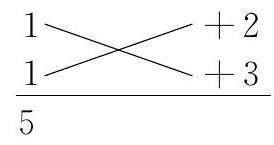
\includegraphics[max width=\textwidth, center]{2024_10_30_bd799899fef40368a068g-035}

其中 2 与 3 是由 6 分解因数产生的,两道交叉的线表示应将线两端的数相乘 (即 $1 \times 3,1 \times 2$ ),然后再相加,横线下的数表示所得的和。如果和等于一次项系数,那么就得到所需要的分解,算式中的第一行与第二行各表示一个因式,第一行 $1+2$ ,表示 $x+2$ ;第二行 $1+3$ ,表示 $x+3$ 。不难看出,这个算式实际上是乘法坚式的省略写法。它被称为十字相乘.

例2 分解因式: $x^{2}-7 x+6$ 。\\
解 这一次把 6 分解为 $2 \times 3$ 是不行的,应当把 6 分解为 $(-1) \times(-6)$ 。由算式\\
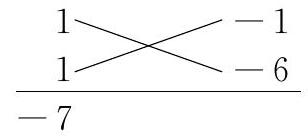
\includegraphics[max width=\textwidth, center]{2024_10_30_bd799899fef40368a068g-035(2)}

得

\begin{align*}
x^{2}-7 x+6=(x-1)(x-6) .
\end{align*}

6 还有两种分解: $6=(-2) \times(-3)=1 \times 6$. 由算式\\
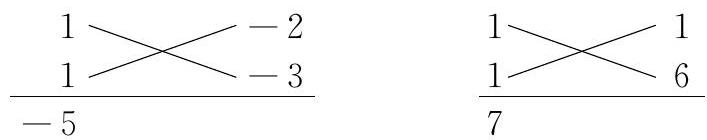
\includegraphics[max width=\textwidth, center]{2024_10_30_bd799899fef40368a068g-035(1)}

可以编出以下两道题:\\
例3 分解因式: $x^{2}-5 x+6$.\\
解

\begin{align*}
x^{2}-5 x+6=(x-2)(x-3)
\end{align*}

例 4 分解因式: $x^{2}+7 x+6$.\\
解

\begin{align*}
x^{2}+7 x+6=(x+1)(x+6)
\end{align*}

\section*{5.2 熟能生巧}
要掌握十字相乘,首先要熟悉整数的因数分解,熟悉有理数的加(减)法,反复练习,熟能生巧。这里再给出几个例题。

例 5 分解因式: $x^{2}+6 x+8$ 。\\
解 $8=2 \times 4$ ,而 $2+4=6$ 。算式为\\
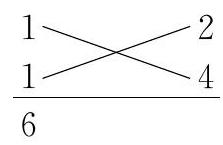
\includegraphics[max width=\textwidth, center]{2024_10_30_bd799899fef40368a068g-036}

所以

\begin{align*}
x^{2}+6 x+8=(x+2)(x+4) .
\end{align*}

例 6 分解因式: $x^{2}-6 x+8$.\\
解 由算式\\
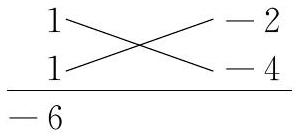
\includegraphics[max width=\textwidth, center]{2024_10_30_bd799899fef40368a068g-036(1)}

得

\begin{align*}
x^{2}-6 x+8=(x-2)(x-4) .
\end{align*}

例7 分解因式: $x^{2}+7 x-8$.\\
解 由算式\\
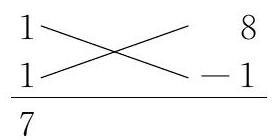
\includegraphics[max width=\textwidth, center]{2024_10_30_bd799899fef40368a068g-036(3)}

得

\begin{align*}
x^{2}+7 x-8=(x+8)(x-1)
\end{align*}

注意:在常数项为正时,两个因数同号(同为正数或同为负数);在常数项为负时,两个因数异号。

例 8 分解因式: $x^{2}-x-6$ 。\\
解 由算式\\
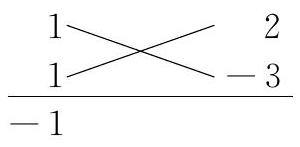
\includegraphics[max width=\textwidth, center]{2024_10_30_bd799899fef40368a068g-036(2)}

得

\begin{align*}
x^{2}-x-6=(x+2)(x-3) .
\end{align*}

有理数的加法,切勿搞错!\\
例 9 分解因式: $x+12-x^{2}$ 。\\
解 按照前面已经说过的办法,先把 $x+12-x^{2}$ "理顺",并提出公因数 -1 ,使首项系数成为 +1 :

\begin{align*}
x+12-x^{2}=-x^{2}+x+12=-\left(x^{2}-x-12\right) .
\end{align*}

由算式\\
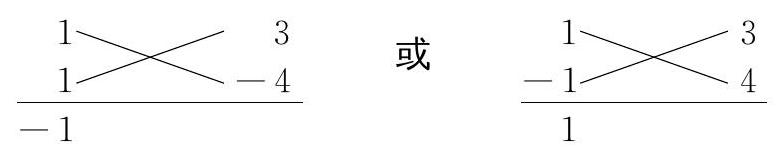
\includegraphics[max width=\textwidth, center]{2024_10_30_bd799899fef40368a068g-037}

得

\begin{align*}
\begin{aligned}
& x+12-x^{2}=-(x+3)(x-4) \\
& x+12-x^{2}=(x+3)(-x+4)
\end{aligned}
\end{align*}

不先提出 -1 , 直接十字相乘也是可以的.

\section*{5.3 再进一步}
前面讨论的是首项系数为 1 的二次三项式. 一般的二次三项式也可以用十字相乘来分解.

例10 分解因式: $6 x^{2}-7 x+2$.\\
解 采用类似的算式:把 6 分解为 $2 \times 3$ ,写在第一列;把 2 分解为 $-1 \times$ ( -2 ), 写在第二列; 然后, 交叉相乘, 把积相加, 最后把得到的和写在横线下面, 即\\
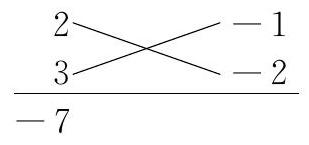
\includegraphics[max width=\textwidth, center]{2024_10_30_bd799899fef40368a068g-037(1)}

这个和恰好是一次项的系数, 于是

\begin{align*}
6 x^{2}-7 x+2=(2 x-1)(3 x-2)
\end{align*}

注:算式中的第一行 $2-1$ ,表示 $2 x-1$ ;第二行 $3-2$ ,表示 $3 x-2$ 。\\
如果得到的和不等于一次项的系数,那么,或者把 $2 \times 3$ 换为 6 的另一种分解,或者把 $-1 \times(-2)$ 换为 2 的另一种分解,或者两者都换。经过多次尝试,就能找出所需要的分解来。

例11 分解因式: $12 x^{2}-11 x-15$.

解 12 与 -15 都有很多种分解. 算式\\
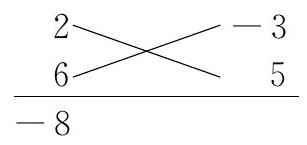
\includegraphics[max width=\textwidth, center]{2024_10_30_bd799899fef40368a068g-038(2)}

是不成的。\\
由算式\\
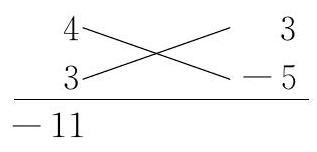
\includegraphics[max width=\textwidth, center]{2024_10_30_bd799899fef40368a068g-038}

得

\begin{align*}
12 x^{2}-11 x-15=(4 x+3)(3 x-5)
\end{align*}

注意:我们总可以假定首项系数是正的,并且它的两个因数都是正数(必要时,将因数 -1 先提出去)。

例12 分解因式: $-6 x^{2}+12-x$ 。\\
解 首先把原式"理顺"(不理顺容易出错):

\begin{align*}
-6 x^{2}+12-x=-\left(6 x^{2}+x-12 .\right)
\end{align*}

由算式\\
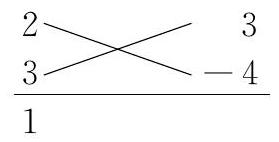
\includegraphics[max width=\textwidth, center]{2024_10_30_bd799899fef40368a068g-038(3)}

得

\begin{align*}
-6 x^{2}+12-x=-(2 x+3)(3 x-4)
\end{align*}

\section*{5.4 二次齐次式}
形如 $a x^{2}+b x y+c y^{2}$ 的多项式,每一项都是 $x$ 与 $y$ 的二次式( $x y$ 中 $x$ 与 $y$ 的次数都是 1 ,所以 $x y$ 的次数是 $1+1=2$ ),称为 $x$ 与 $y$ 的二次齐次式。它的分解与 $x$ 的二次三项式一样,采用十字相乘。

例13 分解因式: $6 x^{2}-7 x y+2 y^{2}$ 。\\
解 由算式\\
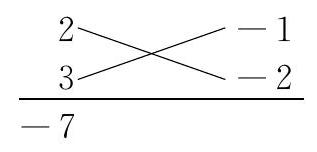
\includegraphics[max width=\textwidth, center]{2024_10_30_bd799899fef40368a068g-038(1)}

得

\begin{align*}
6 x^{2}-7 x y+2 y^{2}=(2 x-y)(3 x-2 y) .
\end{align*}

请注意:算式的第一行 $2-1$ ,表示 $2 x-y$ ;第二行 $3-2$ ,表示 $3 x-2 y$ 。定不要漏掉字母 $y$ 。

例14 分解因式: $x^{2}+144 y^{2}-25 x y$.\\
解

\begin{align*}
x^{2}+144 y^{2}-25 x y=x^{2}-25 x y+144 y^{2},
\end{align*}

由算式\\
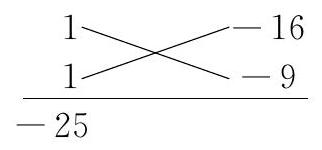
\includegraphics[max width=\textwidth, center]{2024_10_30_bd799899fef40368a068g-039}

得

\begin{align*}
x^{2}+144 y^{2}-25 x y=(x-16 y)(x-9 y) .
\end{align*}

在例 14 中, 144 有多种分解,如果从拆 -25 入手 $(-25=-16-9)$ ,或许更容易奏效. 十字相乘虽然简单,但是,要想做得快,还得依靠实践. 这个问题是可以意会,难于言传的。

\section*{5.5 系数和为零}
如果二次三项式 $a x^{2}+b x+c$ 的系数和

\begin{align*}
a+b+c=0,
\end{align*}

那么

\begin{align*}
a x^{2}+b x+c=(x-1)(a x-c) .
\end{align*}

事实上,因为

\begin{align*}
b=-(a+c),
\end{align*}

这时

\begin{align*}
\begin{aligned}
& (x-1)(a x-c) \\
= & a x^{2}-(a+c) x+c \\
= & a x^{2}+b x+c .
\end{aligned}
\end{align*}

记住这个结论,下面的例题就能迎刃而解了。\\
例15 分解因式: $3 x^{2}+5 x-8$.\\
解

\begin{align*}
3 x^{2}+5 x-8=(x-1)(3 x+8)
\end{align*}

例16 分解因式: $12 x^{2}-19 x y+7 y^{2}$.\\
解

\begin{align*}
12 x^{2}-19 x y+7 y^{2}=(x-y)(12 x-7 y) .
\end{align*}

\section*{小 结}
$x$ 的二次三项式(或 $x$ 与 $y$ 的二次齐次式)应该用十字相乘来分解因式. 方法是把 $x^{2}$ 的系数分解为两个因数的积,把常数项(或 $y^{2}$ 的系数)也分解为两个因数的积, 再把这些因数交叉相乘, 如果所得乘积的和等于 $x$的一次项的系数, 那么就产生出多项式的两个一次因式. 在系数和为零时,必有一个因式是 $x-1$ (或 $x-y$ ),这样,分解的结果可以直接写出来.

\section*{习 题 5}
将以下各式分解因式:\\
$1 x^{2}+12 x+20$.\\
$2 x^{2}-12 x+20$.\\
$3 x^{2}-4 x-5$.\\
$4 x^{2}-9 x-22$.\\
$512 x^{2}-11 x y-15 y^{2}$.\\
$66 x^{2}-13 x+6$.\\
$72 x^{2}+7 x+3$.\\
$82 x^{2}-5 x+3$.\\
$9-20 x y+64 y^{2}+x^{2}$.\\
$10-x^{2}+x+56$.

形如 $a x^{2}+b x y+c y^{2}+d x+e y+f$ 的 $x 、 y$ 的二元二次式也可以用十字相乘法来分解。

\section*{6.1 欲擒故纵}
例1 分解因式: $x^{2}+2 x y-3 y^{2}+3 x+y+2$.\\
解 如果只有二次项 $x^{2}+2 x y-3 y^{2}$, 那么由算式\\
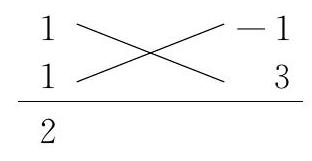
\includegraphics[max width=\textwidth, center]{2024_10_30_bd799899fef40368a068g-041(1)}

得

\begin{align*}
x^{2}+2 x y-3 y^{2}=(x-y)(x+3 y) .
\end{align*}

如果没有含 $y$ 的项, 那么对于多项式 $x^{2}+3 x+2$, 由算式\\
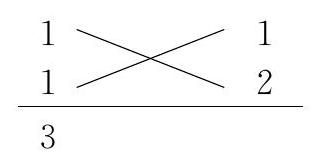
\includegraphics[max width=\textwidth, center]{2024_10_30_bd799899fef40368a068g-041(2)}

得

\begin{align*}
x^{2}+3 x+2=(x+1)(x+2)
\end{align*}

如果没有含 $x$ 的项, 那么对于多项式 $-3 y^{2}+y+2$ ,由算式\\
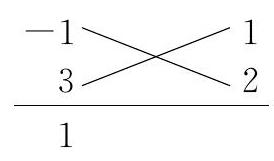
\includegraphics[max width=\textwidth, center]{2024_10_30_bd799899fef40368a068g-041}

得

\begin{align*}
-3 y^{2}+y+2=(-y+1)(3 y+2)
\end{align*}

把以上三个算式"拼"在一起,写成\\
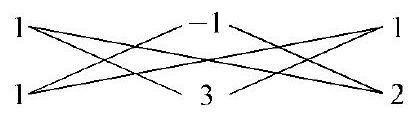
\includegraphics[max width=\textwidth, center]{2024_10_30_bd799899fef40368a068g-042}

便得到所需要的分解:

\begin{align*}
\begin{aligned}
& x^{2}+2 x y-3 y^{2}+3 x+y+2 \\
= & (x-y+1)(x+3 y+2) .
\end{aligned}
\end{align*}

上面的算式称为长十字相乘,式中的三个十字叉就是上面所说的三次十字相乘 (我们省略了横线及横线下面的数). 两次十字相乘就可以确定算式中的 6 个数,第三次十字相乘只需利用已有的数进行检验,必要时把同一列的两个数的位置交换一下。

长十字中的第一行 $1-1+1$ 表示因式 $x-y+1$, 第二行 $1+3+2$ 表示另一个因式 $x+3 y+2$.

为了解决问题,常常先忽略一些条件,导出部分结果,然后再把几方面的部分结果综合起来,这种欲擒故纵的方法在数学中屡见不鲜。

例 2 分解因式: $6 x^{2}-5 x y-6 y^{2}+2 x+23 y-20$ 。\\
解 先进行两次十字相乘,由算式\\
( $x$ )\\
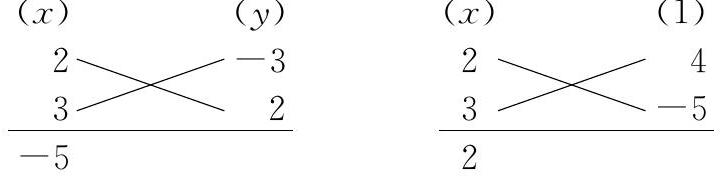
\includegraphics[max width=\textwidth, center]{2024_10_30_bd799899fef40368a068g-042(1)}

得

\begin{align*}
\begin{aligned}
6 x^{2}-5 x y-6 y^{2} & =(2 x-3 y)(3 x+2 y) \\
6 x^{2}+2 x-20 & =(2 x+4)(3 x-5)
\end{aligned}
\end{align*}

为避免混淆,我们在算式中写上 $(x) 、(y) 、(1)$ ,表示相应的列是 $x 、 y$ 的系数或常数项. 然后把两个算式拼成\\
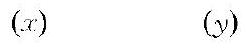
\includegraphics[max width=\textwidth, center]{2024_10_30_bd799899fef40368a068g-042(3)}\\
(1)\\
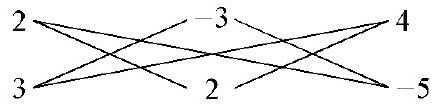
\includegraphics[max width=\textwidth, center]{2024_10_30_bd799899fef40368a068g-042(2)}

检验一下,正好有

\begin{align*}
(-3) \times(-5)+2 \times 4=23,
\end{align*}

于是

\begin{align*}
\begin{aligned}
& 6 x^{2}-5 x y-6 y^{2}+2 x+23 y-20 \\
= & (2 x-3 y+4)(3 x+2 y-5) .
\end{aligned}
\end{align*}

\section*{6. 2 三元齐次}
长十字相乘对于三个字母 $x, y, z$ 的二次齐次式 $a x^{2}+b x y+c y^{2}+d x z+$ $e y z+f z^{2}$ 也同样适合。

例 3 分解因式: $x^{2}-6 x y+9 y^{2}-5 x z+15 y z+6 z^{2}$.\\
解 由算式

得\\
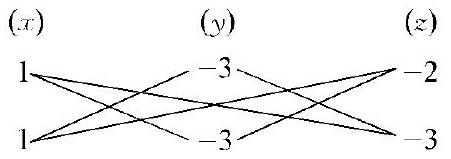
\includegraphics[max width=\textwidth, center]{2024_10_30_bd799899fef40368a068g-043(1)}

\begin{align*}
\begin{aligned}
& x^{2}-6 x y+9 y^{2}-5 x z+15 y z+6 z^{2} \\
= & (x-3 y-2 z)(x-3 y-3 z) .
\end{aligned}
\end{align*}

例 4 已知: $a 、 b 、 c$ 为三角形的三条边,且

\begin{align*}
a^{2}+4 a c+3 c^{2}-3 a b-7 b c+2 b^{2}=0
\end{align*}

求证: $2 b=a+c$.\\
解 由算式\\
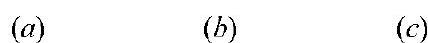
\includegraphics[max width=\textwidth, center]{2024_10_30_bd799899fef40368a068g-043}

得

\begin{align*}
\begin{aligned}
& a^{2}+4 a c+3 c^{2}-3 a b-7 b c+2 b^{2} \\
= & (a-b+3 c)(a-2 b+c) .
\end{aligned}
\end{align*}

于是, 由已知条件, 得

\begin{align*}
(a-b+3 c)(a-2 b+c)=0
\end{align*}

因为三角形的两条边的和大于第三条边, 所以

从而

\begin{align*}
\begin{aligned}
& a-b+3 c \neq 0, \\
& a-2 b+c=0,
\end{aligned}
\end{align*}

即

\begin{align*}
2 b=a+c
\end{align*}

\section*{6.3 项数不全}
如果二次式中缺少一项或几项,长十字相乘仍然可用 (通常更为简单).\\
例 5 分解因式: $x^{2}-y^{2}+5 x+3 y+4$ 。\\
解 由算式\\
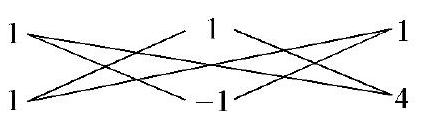
\includegraphics[max width=\textwidth, center]{2024_10_30_bd799899fef40368a068g-044(1)}

得

\begin{align*}
\begin{gathered}
x^{2}-y^{2}+5 x+3 y+4 \\
=(x+y+1)(x-y+4) .
\end{gathered}
\end{align*}

在例 5 中, 如果仅看 $x^{2}-y^{2}$ 与 $x^{2}+5 x+4$, 也可能导出不完全正确的算式\\
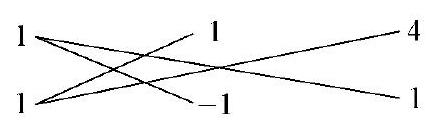
\includegraphics[max width=\textwidth, center]{2024_10_30_bd799899fef40368a068g-044(2)}

在用第三个十字相乘时,可以发现第三列的 4 与 1 应当交换位置.\\
例 6 分解因式: $x^{2}+3 x y+2 y^{2}+2 x+4 y$ 。\\
解 由算式\\
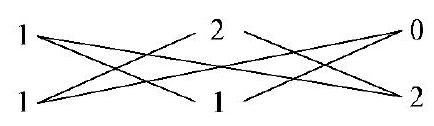
\includegraphics[max width=\textwidth, center]{2024_10_30_bd799899fef40368a068g-044}

得

\begin{align*}
\begin{aligned}
& x^{2}+3 x y+2 y^{2}+2 x+4 y \\
= & (x+2 y)(x+y+2) .
\end{aligned}
\end{align*}

\section*{6.4 能否分解}
二元二次式并不是一定能分解的。如果三个十字相乘不能拼成一个长十字相乘,那么这个二元二次式就不能分解。所以,在编制分解二元二次式的习题时,应当先拟好答案,即两个一次因式,然后把它们相乘,导出一个二元二次式. 换句话说,应当先写出长十字相乘的算式,然后再写出二元二次式. 如果随意地写一个二元二次式,那么多数是不能分解的。

例 $7 m$ 为什么数时, $x^{2}+7 x y-18 y^{2}-5 x+m y-24$ 可以分解为两个一次因式的积?

解 对于多项式 $x^{2}+7 x y-18 y^{2}$ ,有算式\\
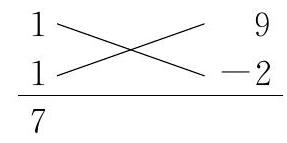
\includegraphics[max width=\textwidth, center]{2024_10_30_bd799899fef40368a068g-045(2)}

对于多项式 $x^{2}-5 x-24$ ,有算式\\
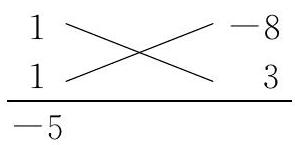
\includegraphics[max width=\textwidth, center]{2024_10_30_bd799899fef40368a068g-045}

这两个算式可以拼成长十字相乘\\
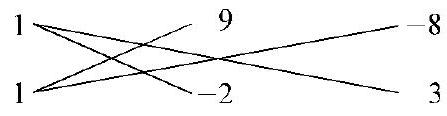
\includegraphics[max width=\textwidth, center]{2024_10_30_bd799899fef40368a068g-045(3)}

或\\
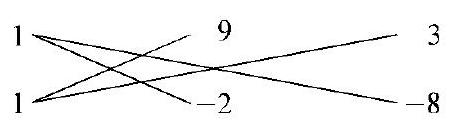
\includegraphics[max width=\textwidth, center]{2024_10_30_bd799899fef40368a068g-045(1)}

对第一个长十字相乘,有

\begin{align*}
9 \times 3+(-2) \times(-8)=43,
\end{align*}

而对第二个长十字相乘,有

\begin{align*}
9 \times(-8)+(-2) \times 3=-78,
\end{align*}

所以, $m=43$ 或 $m=-78$ 时, $x^{2}-7 x y-18 y^{2}-5 x+m y-24$ 才可以分解,并且由第一个长十字相乘,得

\begin{align*}
\begin{aligned}
& x^{2}-7 x y-18 y^{2}-5 x+43 y-24 \\
= & (x+9 y-8)(x-2 y+3),
\end{aligned}
\end{align*}

由第二个长十字相乘,得

\begin{align*}
\begin{aligned}
& x^{2}-7 x y-18 y^{2}-5 x-78 y-24 \\
= & (x+9 y+3)(x-2 y-8) .
\end{aligned}
\end{align*}

$x 、 y$ 的二次式(或 $x 、 y 、 z$ 的二次齐次式)应当用长十字相乘来分解. 长十字相乘由三个十字相乘组成,它们分别表示 $x 、 y$ 的二次齐次式、不含 $x$ 的二次式(或 $y 、 z$ 的二次齐次式)与不含 $y$ 的二次式(或 $z 、 x$ 的二次齐次式)的因式分解。

\section*{习 题 6}
将以下各式分解因式:\\
$1 x^{2}+2 x y+y^{2}+3 x+3 y+2$.\\
$24 x^{2}-14 x y+6 y^{2}-7 x+y-2$.\\
$3 x^{2}-y^{2}-3 z^{2}-2 x z+4 y z$.\\
$42 y^{2}-5 x y+2 x^{2}-a y-a x-a^{2}$.\\
$5 a^{2}-3 b^{2}-3 c^{2}+10 b c-2 c a-2 a b$.\\
$62 a^{2}-7 a b-22 b^{2}-5 a+35 b-3$.\\
$7 x^{2}-2 y^{2}-3 z^{2}+x y+7 y z+2 x z$.\\
$82 x^{2}-6 y^{2}+3 z^{2}-x y+7 x z+7 y z$.\\
$94 x^{2}-9 y^{2}+2 z^{2}+6 x z-3 y z$.\\
$104 x^{2}+2 z^{2}+x y+9 x z+2 y z$.\\
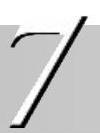
\includegraphics[max width=\textwidth, center]{2024_10_30_bd799899fef40368a068g-047(2)}

我国古代名将岳飞说过:"阵而后战,兵法之常,运用之妙,存乎一心". 因式分解也是这样,学了前面的基本方法,还需要多加练习,灵活运用。

\section*{7.1 善于换元}
例1 分解因式: $x^{6}-28 x^{3}+27$ 。\\
解 如果把 $x^{3}$ 记为 $u$, 那么原式就成为

\begin{align*}
u^{2}-28 u+27
\end{align*}

由算式\\
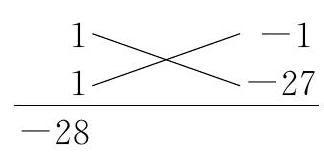
\includegraphics[max width=\textwidth, center]{2024_10_30_bd799899fef40368a068g-047}

得

\begin{align*}
u^{2}-28 u+27=(u-1)(u-27)
\end{align*}

所以

\begin{align*}
x^{6}-28 x^{3}-27
\end{align*}

\begin{align*}
=\left(x^{3}-1\right)\left(x^{3}-27\right)
\end{align*}

\begin{align*}
=(x-1)\left(x^{2}+x+1\right)(x-3)\left(x^{2}+3 x+9\right) .
\end{align*}

其实,不一定明确地把 $x^{3}$ 改记为 $u$ ,只要把 $x^{3}$ 看成一个字母就可以了。\\
例2 分解因式: $\left(x^{2}+4 x+8\right)^{2}+3 x\left(x^{2}+4 x+8\right)+2 x^{2}$ 。\\
解 我们把 $x^{2}+4 x+8$ 看成一个字母,由算式\\
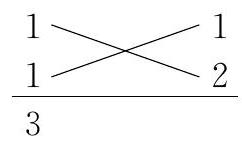
\includegraphics[max width=\textwidth, center]{2024_10_30_bd799899fef40368a068g-047(1)}

得

\begin{align*}
\begin{aligned}
& \left(x^{2}+4 x+8\right)^{2}+3 x\left(x^{2}+4 x+8\right)+2 x^{2} \\
= & \left(x^{2}+4 x+8+x\right)\left(x^{2}+4 x+8+2 x\right)
\end{aligned}
\end{align*}

\begin{align*}
\begin{aligned}
& =\left(x^{2}+5 x+8\right)\left(x^{2}+6 x+8\right) \\
& =(x+2)(x+4)\left(x^{2}+5 x+8\right) .
\end{aligned}
\end{align*}

这里对 $x^{2}+6 x+8$ 再次用十字相乘分解因式,而 $x^{2}+5 x+8$ 在有理数集内不能分解,参见第 11 单元求根公式部分。

例3 证明:四个连续整数的乘积加 1 是整数的平方。\\
证明 设这四个连续整数为

\begin{align*}
x+1, x+2, x+3, x+4,
\end{align*}

则

\begin{align*}
\begin{aligned}
& (x+1)(x+2)(x+3)(x+4)+1 \\
= & {[(x+1)(x+4)][(x+2)(x+3)]+1 } \\
= & \left(x^{2}+5 x+4\right)\left(x^{2}+5 x+6\right)+1 .
\end{aligned}
\end{align*}

我们把 $x+1$ 与 $x+4$ 相乘, $x+2$ 与 $x+3$ 相乘,好处是两个乘积不但二次项相同,而且一次项也是相同的。

把 $x^{2}+5 x+5$ 看成 $u$ ,这时

\begin{align*}
u=x^{2}+5 x+\frac{4+6}{2}
\end{align*}

得

\begin{align*}
\begin{aligned}
& (x+1)(x+2)(x+3)(x+4)+1 \\
= & {\left[\left(x^{2}+5 x+5\right)-1\right]\left[\left(x^{2}+5 x+5\right)+1\right]+1 } \\
= & \left(x^{2}+5 x+5\right)^{2}-1+1 \\
= & \left(x^{2}+5 x+5\right)^{2},
\end{aligned}
\end{align*}

这是一个平方数。\\
在本题中把 $x^{2}+5 x$ 或 $x^{2}+5 x+4$ 看成一个字母也是可以的,但切勿把 $(x+1)(x+2)(x+3)(x+4)$ 全部乘出来写成 $x$ 的四次式,那样做的结果是破坏了规律性,难以下手。

例 4 分解因式: $4(x+5)(x+6)(x+10)(x+12)-3 x^{2}$ 。\\
解 第一项的四个因式以将 $x+5$ 与 $x+12$ 相乘、 $x+6$ 与 $x+10$ 相乘为好,这时不仅二次项相同,而且常数项也相同,于是

\begin{align*}
\begin{aligned}
& 4(x+5)(x+6)(x+10)(x+12)-3 x^{2} \\
= & 4\left(x^{2}+17 x+60\right)\left(x^{2}+16 x+60\right)-3 x^{2} \\
= & 4\left[\left(x^{2}+16 x+60\right)+x\right]\left(x^{2}+16 x+60\right)-3 x^{2} \\
= & 4\left(x^{2}+16 x+60\right)^{2}+4 x\left(x^{2}+16 x+60\right)-3 x^{2} \\
= & {\left[2\left(x^{2}+16 x+60\right)-x\right]\left[2\left(x^{2}+16 x+60\right)+3 x\right] } \\
= & \left(2 x^{2}+31 x+120\right)\left(2 x^{2}+35 x+120\right)
\end{aligned}
\end{align*}

[把 $x^{2}+16 x+60$ 看作 $u$ ]\\
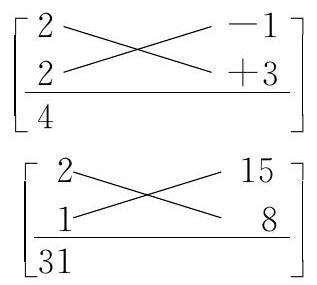
\includegraphics[max width=\textwidth, center]{2024_10_30_bd799899fef40368a068g-048}\\
$=(2 x+15)(x+8)\left(2 x^{2}+35 x+120\right)$.

\section*{7.2 主次分清}
例 5 分解因式: $a^{2} b-a b^{2}+a^{2} c-a c^{2}-3 a b c+b^{2} c+b c^{2}$.\\
解 这个多项式是 $a 、 b 、 c$ 的三次式,项数多,似乎无从下手,解决它的方法却是最基本的:把 $a$ 当作主要字母,也就是把这个多项式看成 $a$ 的二次式,按 $a$ 降幂排列整理为

\begin{align*}
(b+c) a^{2}-\left(b^{2}+c^{2}+3 b c\right) a+\left(b^{2} c+b c^{2}\right)
\end{align*}

然后用十字相乘进行分解,这里的"常数项"为

\begin{align*}
b^{2} c+b c^{2}=b c(b+c)
\end{align*}

由算式

\begin{align*}
\frac{-\begin{array}{c}
-(b+c) \\
-b c
\end{array}}{-(b+c)^{2}-b c=-b^{2}-c^{2}-3 b c}
\end{align*}

得

\begin{align*}
\begin{aligned}
& a^{2} b-a b^{2}+a^{2} c-a c^{2}-3 a b c+b^{2} c+b c^{2} \\
= & {[a-(b+c)][(b+c) a-b c] } \\
= & (a-b-c)(a b+a c-b c) .
\end{aligned}
\end{align*}

注:这个问题还有一个解法,见习题 9 第 3 题。\\
例 6 分解因式: $y(y+1)\left(x^{2}+1\right)+x\left(2 y^{2}+2 y+1\right)$ 。\\
解 这是 $x$ 的二次式,原式化为

\begin{align*}
y(y+1) x^{2}+\left(2 y^{2}+2 y+1\right) x+y(y+1) .
\end{align*}

由算式

得

\begin{align*}
\begin{aligned}
& y(y+1)\left(x^{2}+1\right)+x\left(2 y^{2}+2 y+1\right) \\
= & {[y x+(y+1)][(y+1) x+y] } \\
= & (y x+y+1)(y x+x+y) .
\end{aligned}
\end{align*}

例7 分解因式: $a b\left(x^{2}-y^{2}\right)-\left(a^{2}-b^{2}\right)(x y+1)-\left(a^{2}+b^{2}\right)(x+y)$.

解 以 $a 、 b$ 为主要字母,这个多项式是 $a 、 b$ 的二次齐次式,把它整理成

\begin{align*}
\begin{aligned}
& b^{2}[(x y+1)-(x+y)]+a b\left(x^{2}-y^{2}\right)-a^{2}[(x+y)+(x y+1)] \\
= & b^{2}[(x y-x)-(y-1)]+a b\left(x^{2}-y^{2}\right)-a^{2}[(x+x y)+(y+1)] \\
= & b^{2}[x(y-1)-(y-1)]+a b\left(x^{2}-y^{2}\right)-a^{2}[x(y+1)+(y+1)] \\
= & b^{2}(x-1)(y-1)+a b\left(x^{2}-y^{2}\right)-a^{2}(x+1)(y+1) .
\end{aligned}
\end{align*}

(注:我们把 $b^{2}$ 与 $a^{2}$ 的系数分解是为了进行十字相乘, $a b$ 的系数不必分解)

由算式

得

\begin{align*}
\begin{aligned}
\text { 原式 } & =[(x-1) b-(y+1) a][(y-1) b-(x+1) a] \\
& =(b x-b-a y-a)(b y-b+a x+a) .
\end{aligned}
\end{align*}

这题按 $a$ 降幂排列也未尝不可,但是首项系数有一个负号。

\section*{7.3 一题两解}
例 8 分解因式: $x^{2}+2(a+b) x-3 a^{2}+10 a b-3 b^{2}$ 。\\
解法一 这是 $x$ 的二次式,"常数项"可分解为

\begin{align*}
\begin{aligned}
& -3 a^{2}+10 a b-3 b^{2} \\
= & -\left(3 a^{2}-10 a b+3 b^{2}\right) \\
= & -(3 a-b)(a-3 b) .
\end{aligned}
\end{align*}

再对整个式子运用十字相乘,由算式

得

\begin{align*}
\begin{gathered}
\frac{1}{-(a-3 b)+3 a-b=2 a+2 b} \begin{array}{c}
3 a-b \\
-(a-3 b)
\end{array} \\
x^{2}+2(a+b) x-3 a^{2}+10 a b-3 b^{2} \\
=(x+3 a-b)(x-a+3 b) .
\end{gathered}
\end{align*}

解法二 把 $x^{2}+2(a+b) x-3 a^{2}+10 a b-3 b^{2}$ 看成 $x 、 a 、 b$ 的二次齐次式,对它采用长十字相乘,由算式\\
(x)\\
(a)\\
(b)

得\\
原式 $=(x-a+3 b)(x+3 a-b)$.

\section*{7. 4 展开处理}
例9 分解因式: $(a x+b y)^{2}+(a y-b x)^{2}$ 。\\
解 这道题必须展开处理。

\begin{align*}
\begin{aligned}
& (a x+b y)^{2}+(a y-b x)^{2} \\
= & a^{2} x^{2}+2 a b x y+b^{2} y^{2}+a^{2} y^{2}-2 a b x y+b^{2} x^{2} \\
= & a^{2} x^{2}+b^{2} y^{2}+a^{2} y^{2}+b^{2} x^{2} \\
= & \left(a^{2} x^{2}+a^{2} y^{2}\right)+\left(b^{2} y^{2}+b^{2} x^{2}\right) \\
= & a^{2}\left(x^{2}+y^{2}\right)+b^{2}\left(x^{2}+y^{2}\right) \\
= & \left(a^{2}+b^{2}\right)\left(x^{2}+y^{2}\right) .
\end{aligned}
\end{align*}

这个等式表明两个平方和 $\left(a^{2}+b^{2}\right.$ 与 $\left.x^{2}+y^{2}\right)$ 的积仍然是平方和.\\
例10 分解因式: $a^{4}+4^{4}+(a-4)^{4}$ 。\\
解 为更加对称起见,我们令

\begin{align*}
x=a-2,
\end{align*}

于是 $\quad a^{4}+4^{4}+(a-4)^{4}$

\begin{align*}
\begin{aligned}
= & (x+2)^{4}+(x-2)^{4}+4^{4} \\
= & \left(x^{2}+4 x+4\right)^{2}+\left(x^{2}-4 x+4\right)^{2}+4^{4} \\
= & \left(x^{4}+16 x^{2}+16+8 x^{3}+8 x^{2}+32 x\right)+\left(x^{4}+16 x^{2}+16-8 x^{3}+8 x^{2}\right. \\
& -32 x)+4^{4} \\
= & 2\left(x^{4}+24 x^{2}+16\right)+256 \\
= & 2\left(x^{4}+24 x^{2}+144\right) \\
= & 2\left(x^{2}+12\right)^{2} \\
= & 2\left[(a-2)^{2}+12\right]^{2} \\
= & 2\left(a^{2}-4 a+16\right)^{2} .
\end{aligned}
\end{align*}

本例是以后第 11 单元例 12 的特殊情况.\\
例 11 分解因式: $x y z\left(x^{3}+y^{3}+z^{3}\right)-y^{3} z^{3}-z^{3} x^{3}-x^{3} y^{3}$ 。

\begin{align*}
x y z\left(x^{3}+y^{3}+z^{3}\right)-y^{3} z^{3}-z^{3} x^{3}-x^{3} y^{3}
\end{align*}

\begin{align*}
\begin{aligned}
& =x^{4} y z+x y^{4} z+x y z^{4}-y^{3} z^{3}-z^{3} x^{3}-x^{3} y^{3} \\
& =\left(x^{4} y z-y^{3} z^{3}\right)+\left(x y^{4} z-x^{3} y^{3}\right)+\left(x y z^{4}-z^{3} x^{3}\right) \\
& =y z\left(x^{4}-y^{2} z^{2}\right)+x y^{3}\left(y z-x^{2}\right)+x z^{3}\left(y z-x^{2}\right) \\
& =y z\left(x^{2}+y z\right)\left(x^{2}-y z\right)-x y^{3}\left(x^{2}-y z\right)-x z^{3}\left(x^{2}-y z\right) \\
& =\left(x^{2}-y z\right)\left[y z\left(x^{2}+y z\right)-x y^{3}-x z^{3}\right] \\
& =\left(x^{2}-y z\right)\left[x^{2} y z+y^{2} z^{2}-x y^{3}-x z^{3}\right] \\
& =\left(x^{2}-y z\right)\left[\left(x^{2} y z-x y^{3}\right)+\left(y^{2} z^{2}-x z^{3}\right)\right] \\
& =\left(x^{2}-y z\right)\left[x y\left(x z-y^{2}\right)+z^{2}\left(y^{2}-x z\right)\right] \\
& =\left(x^{2}-y z\right)\left(y^{2}-x z\right)\left(z^{2}-x y\right) .
\end{aligned}
\end{align*}

在这个例子中经过两次展开重新组合,每一组中的两项符号相反。\\
以后,第 10 单元有处理这种"对称式"的方法。

\section*{7.5 巧运匠心}
例12 分解因式: $(a+b)^{2}(a b-1)+1$ 。\\
解 把前一项拆为两项,即

\begin{align*}
\begin{aligned}
& (a+b)^{2}(a b-1)+1 \\
= & (a+b)^{2} a b-(a+b)^{2}+1 .
\end{aligned}
\end{align*}

如果是 $x$ 的二次式

\begin{align*}
(a+b)^{2} a b x^{2}-(a+b)^{2} x+1,
\end{align*}

那么可以用十字相乘来分解,由算式

\begin{align*}
\left.\begin{array}{c}
a(a+b) \\
b(a+b)
\end{array} \longrightarrow \begin{array}{c}
-1 \\
-1
\end{array}\right]
\end{align*}

得

\begin{align*}
\begin{aligned}
& (a+b)^{2} a b x^{2}-(a+b)^{2} x+1 \\
= & {[a(a+b) x-1][b(a+b) x-1] . }
\end{aligned}
\end{align*}

在上式中令 $x=1$ ,即可得

\begin{align*}
\begin{aligned}
& (a+b)^{2} a b-(a+b)+1 \\
= & {[a(a+b)-1][b(a+b)-1] } \\
= & \left(a^{2}+a b-1\right)\left(a b+b^{2}-1\right) .
\end{aligned}
\end{align*}

这个例子很有趣,有字母 $x$ 时可以十字相乘,没有 $x$ 时反而不容易看出

它也可以十字相乘.\\
例 13 将 $5^{1985}-1$ 分解为三个大于 $5^{100}$ 的因数相乘。\\
解 令 $x=5^{397}$ ,则

\begin{align*}
\begin{align*}
& 5^{1985}-1 \\
= & x^{5}-1 \\
= & (x-1)\left(x^{4}+x^{3}+x^{2}+x+1\right)
\end{align*} \tag{12}
\end{align*}

在一般情况下, $x^{4}+x^{3}+x^{2}+x+1$ 是一个有理数集内的既约多项式。现在 $x=5^{397}$ ,所以 $5 x=5^{398}=\left(5^{199}\right)^{2}$ 是一个平方数。在这一特殊情况中,我们可以设法把 $x^{4}+x^{3}+x^{2}+x+1$ 化为两个代数式的平方差。如果前一个式的平方是

\begin{align*}
\left(x^{2}+x+1\right)^{2}=x^{4}+2 x^{3}+3 x^{2}+2 x+1
\end{align*}

那么这时还剩下

\begin{align*}
\begin{aligned}
& \left(x^{4}+x^{3}+x^{2}+x+1\right)-\left(x^{4}+2 x^{3}+3 x^{2}+2 x+1\right) \\
= & -x^{3}-2 x^{2}-x \\
= & -x\left(x^{2}+2 x+1\right) \\
= & -x(x+1)^{2},
\end{aligned}
\end{align*}

这样处理不能获得两个代数式的平方差。\\
应当使后一项成为 $-5 x(x+1)^{2}$ ,显然 $5 x(x+1)^{2}$ 是自然数的平方!这时,另一项为

\begin{align*}
\begin{aligned}
& x^{4}+x^{3}+x^{2}+x+1-\left[-5 x(x+1)^{2}\right] \\
= & x^{4}+x^{3}+x^{2}+x+1+5 x\left(x^{2}+2 x+1\right) \\
= & x^{4}+x^{3}+x^{2}+x+1+5 x^{3}+10 x^{2}+5 x \\
= & x^{4}+6 x^{3}+11 x^{2}+6 x+1 \\
= & \left(x^{2}+3 x+1\right)^{2},
\end{aligned}
\end{align*}

这是一个平方。\\
因此,可得

\begin{align*}
\begin{aligned}
& 5^{1985}-1 \\
= & (x-1)\left(x^{4}+x^{3}+x^{2}+x+1\right) \\
= & (x-1)\left[\left(x^{2}+3 x+1\right)^{2}-5 x(x+1)^{2}\right] \\
= & (x-1)\left\{\left(x^{2}+3 x+1\right)^{2}-\left[5^{199}(x+1)\right]^{2}\right\} \\
= & (x-1)\left[x^{2}+3 x+1+5^{199}(x+1)\right]\left[x^{2}+3 x+1-5^{199}(x+1)\right],
\end{aligned}
\end{align*}

而且这三个因数都大于 $5^{100}$.

\section*{小 结}
每道复杂问题的解法都可以分为若干步,每一步都是一个简单的问题. 因此, 要解决复杂的问题, 首先要会解决简单的问题. 登高必自卑, 行远必自迩. 彻底、纯熟地掌握前面所说的基本方法即提、代、分、拆、十字相乘等,"难题"也就不太难了。

为了确定解题的途径与步骤,应当善于换元,把某个多项式整个看作一个字母, 应当分清主次, 以一两个字母作主要字母, 按主要字母的降幂排列,将式子理顺;必要时,应适当展开括号或拆项,重新分组。当然 "运用之妙,存乎一心",要根据情况,注意规律,工丂运匠心,不可执一不化,生搬硬套。

除了前面所说的基本方法, $x$ 的一元多项式 $f(x)$ 可以用第 8 单元的方法求出它的一次因式; $x 、 y 、 z$ 的轮换式可以用第 10 单元的方法分解;第 9 单元介绍待定系数法, 可以确定 $x$ 的四次多项式的二次因式; 第 11单元介绍实数集与负数集内的分解以及如何判定 $x$ 的多项式是否有二次因式 $x^{2}+x+1$. 在因式分解中, 应当分清问题的类型, 选用适当的方法。

最后,必须注意分解到底,即应当把原式分解为既约多项式的乘积,不能半途而废。

在 12 单元将介绍判别一个多项式是否为既约多项式的方法.\\
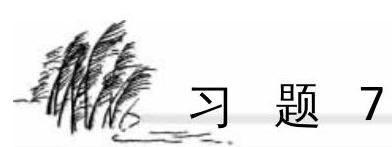
\includegraphics[max width=\textwidth, center]{2024_10_30_bd799899fef40368a068g-054}

将以下各式分解因式:\\
1 $x^{4}-10 x^{2} y^{2}+9 y^{4}$ 。\\
$2 x^{6}-19 x^{3} y^{3}-216 y^{6}$.\\
$3 x^{4}-2\left(a^{2}+b^{2}\right) x^{2}+\left(a^{2}-b^{2}\right)^{2}$.\\
$4\left[\left(x^{2}+y^{2}\right)\left(a^{2}+b^{2}\right)+4 a b x y\right]^{2}-4\left[x y\left(a^{2}+b^{2}\right)+a b\left(x^{2}+y^{2}\right)\right]^{2}$.\\
$5(a x+b y+a y)^{2}+(b x-a y)(a x+b y+a y)+(b x-a y)^{2}$.\\
$6(1+y)^{2}-2 x^{2}\left(1+y^{2}\right)+x^{4}(1-y)^{2}$.\\
$7 a b c x^{2}+\left(a^{2} b^{2}+c^{2}\right) x+a b c$.\\
$8(a-b) x^{2}+2 a x+a+b$.\\
$9 x^{2}+(a+b+c) x+(a+b) c$.\\
$10 a^{2} b c+a c^{2}+a c d-a b d-c d-d^{2}$.\\
$11 x^{4}-x^{2}\left(a^{2}+1\right)+a^{2}$.\\
$12 x^{4}+x^{2}-2 a x+1-a^{2}$.\\
$13(a y+b x)^{3}+(a x+b y)^{3}-\left(a^{3}+b^{3}\right)\left(x^{3}+y^{3}\right)$.\\
$14(x+1)(x+3)(x+5)(x+7)+15$.\\
$15(a-1)(a-2)(a-3)(a-4)-24$.\\
$16\left(x^{2}+x\right)^{2}+4\left(x^{2}+x\right)-12$.\\
$17\left(x^{2}+x+4\right)^{2}+8 x\left(x^{2}+x+4\right)+15 x^{2}$.\\
$182\left(x^{2}+6 x+1\right)^{2}+5\left(x^{2}+6 x+1\right)\left(x^{2}+1\right)+2\left(x^{2}+1\right)^{2}$.\\
$19\left(x^{2}+x\right)^{2}-14\left(x^{2}+x\right)+24$.\\
$20\left(x^{2}+4 x+8\right)^{2}+3 x\left(x^{2}+4 x+8\right)+2 x^{2}$.\\
$21\left(x^{2}+x+1\right)\left(x^{2}+x+2\right)-12$.\\
$22\left(x^{2}+6 x+8\right)\left(x^{2}+14 x+48\right)+12$.

设 $a_{n} x^{n}+a_{n-1} x^{n-1}+\cdots+a_{1} x+a_{0}$ 为 $x$ 的 $n$ 次多项式, 本单元介绍求它的一次因式的方法。

\section*{8.1 余数定理}
我们用 $f(x)$ 表示多项式 $a_{n} x^{n}+a_{n-1} x^{n-1}+\cdots+a_{1} x+a_{0}$ ,用 $f(a)$ 表示这个多项式在 $x=a$ 时的值。例如,在 $f(x)=x^{3}+6 x^{2}+11 x+6$ 时,可得

\begin{align*}
\begin{aligned}
& f(1)=1+6+11+6=24 \\
& f(-1)=-1+6-11+6=0 \\
& f(+2)=8+24+22+6=60
\end{aligned}
\end{align*}

如果我们用一次多项式 $x-c$ 作除式去除多项式 $f(x)$ ,那么余式是一个数。设这时商式为多项式 $g(x)$ ,余式(余数)为 $r$ ,则

\begin{align*}
f(x)=(x-c) g(x)+r, \tag{1}
\end{align*}

即被除式等于除式乘以商式再加余式。\\
在(1)式中令 $x=c$ ,便得到

\begin{align*}
f(c)=0+r=r,
\end{align*}

因此,我们有\\
$x-c$ 除 $f(x)$ 时, 所得的余数为 $f(c)$ 。\\
这个结论称为余数定理。\\
如果余数为 0 ,那么 $f(x)$ 被 $x-c$ 整除,也就是 $x-c$ 是 $f(x)$ 的因式。反过来,如果 $x-c$ 是 $f(x)$ 的因式,那么 $f(x)$ 被 $x-c$ 整除,余数为 0 。因此,我们有

如果 $f(c)=0$, 那么 $x-c$ 是 $f(x)$ 的因式。反过来, 如果 $x-c$ 是 $f(x)$ 的因式,那么 $f(c)=0$ 。

例1 分解因式: $f(x)=x^{3}+6 x^{2}+11 x+6$.

解 因为 $f(-1)=0$ ,根据上面的结论 $x-(-1)=x+1$ 是它的一次因式。知道这个因式后,施行除法就可以把商式求出来。不过,我们也可以不用除法,直接去分组分解。这里分组是"有的放矢"的,每一组都有一个因式 $x+$ 1 ,即

\begin{align*}
\begin{aligned}
& x^{3}+6 x^{2}+11 x+6 \\
= & \left(x^{3}+x^{2}\right)+\left(5 x^{2}+5 x\right)+(6 x+6) \\
= & x^{2}(x+1)+5 x(x+1)+6(x+1) \\
= & (x+1)\left(x^{2}+5 x+6\right) \\
= & (x+1)(x+2)(x+3) .
\end{aligned}
\end{align*}

例 2 设 $f(x)=2 x^{3}-5 x^{2}+5 x-3$, 计算 $f(1), f(-1), f\left(\frac{3}{2}\right)$, 并把 $f(x)$ 分解.

解

\begin{align*}
\begin{aligned}
& f(1)=2-5+5-3=-1 \\
& f(-1)=-2-5-5-3=-15 \\
& f\left(\frac{3}{2}\right)=2 \cdot\left(\frac{3}{2}\right)^{3}-5 \cdot\left(\frac{3}{2}\right)^{2}+5 \cdot\left(\frac{3}{2}\right)-3 \\
& \quad=\frac{27}{4}-\frac{45}{4}+\frac{15}{2}-3=0
\end{aligned}
\end{align*}

可知 $x-\frac{3}{2}$ 是 $f(x)$ 的一次因式. 为了避免分数运算,我们把 $x-\frac{3}{2}$ 乘以 2 得 $2 x-3,2 x-3$ 仍然是 $f(x)$ 的一次因式。

现在把 $f(x)$ 分组分解,注意使每组都有因式 $2 x-3$ (也就是同一组中两项的系数比为 $2:(-3))$ :

\begin{align*}
\begin{aligned}
& 2 x^{3}-5 x^{2}+5 x-3 \\
= & \left(2 x^{3}-3 x^{2}\right)-\left(2 x^{2}-3 x\right)+(2 x-3) \\
= & x^{2}(2 x-3)-x(2 x-3)+(2 x-3) \\
= & (2 x-3)\left(x^{2}-x+1\right) .
\end{aligned}
\end{align*}

\section*{8.2 有理根的求法}
如果 $f(c)=0$ ,那么就说 $c$ 是多项式 $f(x)$ 的根。因此,在 $c$ 是 $f(x)$ 的根时, $x-c$ 是 $f(x)$ 的因式。问题是怎样求出 $f(x)$ 的根?

我们假定 $f(x)=a_{n} x^{n}+a_{n-1} x^{n-1}+\cdots+a_{1} x+a_{0}$ 是整系数多项式,也就

是说 $a_{n}, a_{n-1}, \cdots, a_{1}, a_{0}$ 都是整数。又设有理数 $c=\frac{p}{q}$ 是 $f(x)$ 的根,这里 $p 、$ $q$ 是两个互质的整数。

由于 $f(c)=0$ ,即

\begin{align*}
a_{n}\left(\frac{p}{q}\right)^{n}+a_{n-1}\left(\frac{p}{q}\right)^{n-1}+\cdots+a_{1}\left(\frac{p}{q}\right)+a_{0}=0
\end{align*}

两边同乘 $q^{n}$ 得

\begin{align*}
a_{n} p^{n}+a_{n-1} p^{n-1} q+\cdots+a_{1} p q^{n-1}+a_{0} q^{n}=0 \tag{2}
\end{align*}

(2)式右边被 $p$ 整除( 0 被任何一个不等于 0 的数整除),所以它的左边也被 $p$ 整除。显然,左边的前 $n$ 项都被 $p$ 整除,所以最后一项 $a_{0} q^{n}$ 也被 $p$ 整除,但 $p$ 与 $q$ 互质,所以 $p$ 整除 $a_{0}$ ,即 $p$ 是 $a_{0}$ 的因数(约数)。同样地, $q$ 应当整除 $a_{n} p^{n}$ ,从而 $q$ 是 $a_{n}$ 的因数(约数)。于是,可得

有理根 $c=\frac{p}{q}$ 的分子 $p$ 是常数项 $a_{0}$ 的因数, 分母 $q$ 是首项系数 $a_{n}$ 的因数.\\
例3 分解因式: $f(x)=2 x^{3}-x^{2}-5 x-2$ 。\\
解 $a_{0}=-2$ 的因数是 $\pm 1, \pm 2, a_{n}=2$ 的因数是 $\pm 1, \pm 2$ 。因此, $f(x)$的有理根只可能是 $\pm 1, \pm 2$ (分母为 1 ),$\pm \frac{1}{2}$ 。因为

\begin{align*}
\begin{gathered}
f(1)=2-1-5-2=-6 \\
f(-1)=-2-1+5-2=0
\end{gathered}
\end{align*}

于是 -1 是 $f(x)$ 的一个根, 从而 $x+1$ 是 $f(x)$ 的因式, 可得

\begin{align*}
\begin{aligned}
& 2 x^{3}-x^{2}-5 x-2 \\
= & \left(2 x^{3}+2 x^{2}\right)-\left(3 x^{2}+3 x\right)-(2 x+2) \\
= & 2 x^{2}(x+1)-3 x(x+1)-2(x+1) \\
= & \left(2 x^{2}-3 x-2\right)(x+1) \\
= & (x-2)(2 x+1)(x+1) .
\end{aligned}
\end{align*}

例4 分解因式: $f(x)=3 x^{3}+x^{2}+x-2$ 。\\
解 $a_{0}=-2$ 的因数为 $\pm 1, \pm 2, a_{n}=3$ 的正因数为 $+1,+3$ (我们可以认为 $\frac{p}{q}$ 的分母 $q$ 是正的, 因此 $a_{0}$ 的因数有正有负, $a_{n}$ 的因数可只取正的)。所以, $f(x)$ 的有理根只可能是 $\pm 1, \pm 2, \pm \frac{1}{3}, \pm \frac{2}{3}$.

由于

\begin{align*}
\begin{aligned}
f\left(\frac{2}{3}\right) & =3 \cdot\left(\frac{2}{3}\right)^{3}+\left(\frac{2}{3}\right)^{2}+\left(\frac{2}{3}\right)-2 \\
& =\frac{8}{9}+\frac{4}{9}+\frac{2}{3}-2=0
\end{aligned}
\end{align*}

所以 $x-\frac{2}{3}$ 是 $f(x)$ 的因式, 从而 $3 x-2$ 是 $f(x)$ 的因式, 可得

\begin{align*}
\begin{aligned}
& f(x)=3 x^{3}+x^{2}+x-2 \\
= & \left(3 x^{3}-2 x^{2}\right)+\left(3 x^{2}-2 x\right)+(3 x-2) \\
= & x^{2}(3 x-2)+x(3 x-2)+(3 x-2) \\
= & (3 x-2)\left(x^{2}+x+1\right) .
\end{aligned}
\end{align*}

例 5 分解因式: $f(x)=6 x^{4}+5 x^{3}+3 x^{2}-3 x-2$.\\
解 $a_{0}=-2$ 的因数为 $\pm 1, \pm 2, a_{n}=6$ 的正因数为 $1,2,3,6$ 。所以, $f(x)$ 的有理根只可能为

\begin{align*}
\pm 1, \pm 2, \pm \frac{1}{2}, \pm \frac{1}{3}, \pm \frac{2}{3}, \pm \frac{1}{6}
\end{align*}

经检验 $c=-\frac{1}{2}$ 是一个根,所以 $2 x+1$ 是 $f(x)$ 的因式,可得

\begin{align*}
\begin{aligned}
& 6 x^{4}+5 x^{3}+3 x^{2}-3 x-2 \\
= & \left(6 x^{4}+3 x^{3}\right)+\left(2 x^{3}+x^{2}\right)+\left(2 x^{2}+x\right)-(4 x+2) \\
= & (2 x+1)\left(3 x^{3}+x^{2}+x-2\right) \\
= & (2 x+1)(3 x-2)\left(x^{2}+x+1\right) .
\end{aligned}
\end{align*}

[利用例4]

\section*{8. 3 首 1 多项式}
对于首项系数为 1 的整系数多项式 $f(x)$ ,问题更加简单. 这时 $q=1$ ,有理根都是整数根。

例 6 分解因式: $x^{6}+2 x^{5}+3 x^{4}+4 x^{3}+3 x^{2}+2 x+1$ 。\\
解 本题有理根只可能为 $\pm 1 .+1$ 当然不可能为根(因为多项式的系数全是正的),经检验 -1 是根,所以原式有因式 $x+1$ ,并且

\begin{align*}
\begin{aligned}
& x^{6}+2 x^{5}+3 x^{4}+4 x^{3}+3 x^{2}+2 x+1 \\
= & \left(x^{6}+x^{5}\right)+\left(x^{5}+x^{4}\right)+\left(2 x^{4}+2 x^{3}\right)+\left(2 x^{3}+2 x^{2}\right)+\left(x^{2}+x\right)+(x+1) \\
= & (x+1)\left(x^{5}+x^{4}+2 x^{3}+2 x^{2}+x+1\right) .
\end{aligned}
\end{align*}

容易验证 -1 也是 $x^{5}+x^{4}+2 x^{3}+2 x^{2}+x+1$ 的根,并且

\begin{align*}
\begin{aligned}
& x^{5}+x^{4}+2 x^{3}+2 x^{2}+x+1 \\
= & \left(x^{5}+x^{4}\right)+\left(2 x^{3}+2 x^{2}\right)+(x+1) \\
= & (x+1)\left(x^{4}+2 x^{2}+1\right) \\
= & (x+1)\left(x^{2}+1\right)^{2},
\end{aligned}
\end{align*}

所以

\begin{align*}
\begin{aligned}
& x^{6}+2 x^{5}+3 x^{4}+4 x^{3}+3 x^{2}+2 x+1 \\
= & (x+1)^{2}\left(x^{2}+1\right)^{2} .
\end{aligned}
\end{align*}

例7 分解因式: $x^{3}-9 x^{2}+26 x-24$.\\
解 有理根只可能为

\begin{align*}
\pm 1, \pm 2, \pm 3, \pm 4, \pm 6, \pm 8, \pm 12, \pm 24
\end{align*}

经检验, 2 是根, 所以原式有因式 $x-2$, 并且

\begin{align*}
\begin{aligned}
& x^{3}-9 x^{2}+26 x-24 \\
= & \left(x^{3}-2 x^{2}\right)-\left(7 x^{2}-14 x\right)+(12 x-24) \\
= & (x-2)\left(x^{2}-7 x+12\right) \\
= & (x-2)(x-3)(x-4) .
\end{aligned}
\end{align*}

例 8 分解因式: $x^{3}-9 x^{2} y+26 x y^{2}-24 y^{3}$ 。\\
解

\begin{align*}
\begin{aligned}
& x^{3}-9 x^{2} y+26 x y^{2}-24 y^{3} \\
= & (x-2 y)(x-3 y)(x-4 y) .
\end{aligned}
\end{align*}

这只不过是在上题的解答上添上几个 $y$ 而已。\\
例 9 分解因式: $-24 y^{3}+26 y^{2}-9 y+1$ 。\\
解 $a_{n}=-24$ ,但 $a_{0}=1$ 。为了避免分数计算的麻烦,我们把原式改为升幂排列

\begin{align*}
1-9 y+26 y^{2}-24 y^{3}
\end{align*}

如果与例 8 比较一下, 就会发现两者实质上是相同的, 即在例 8 中令 $x=$ 1,便得到

\begin{align*}
\begin{aligned}
& 1-9 y+26 y^{2}-24 y^{3} \\
= & (1-2 y)(1-3 y)(1-4 y) .
\end{aligned}
\end{align*}

例10 分解因式: $x^{3}-\frac{5}{3} x^{2}-\frac{11}{3} x-1$.\\
解 原式不是整系数多项式,但可以先提取 $\frac{1}{3}$ ,然后再按上面的办法分解,得

\begin{align*}
x^{3}-\frac{5}{3} x^{2}-\frac{11}{3} x-1
\end{align*}

\begin{align*}
\begin{aligned}
& =\frac{1}{3}\left(3 x^{3}-5 x^{2}-11 x-3\right) \\
& =\frac{1}{3}(x+1)(x-3)(3 x+1)
\end{aligned}
\end{align*}

\section*{8.4 字母系数}
例11 分解因式: $x^{3}-(a+b+c) x^{2}+(a b+b c+c a) x-a b c$ 。\\
解 常数项 $-a b c$ 的因数为

\begin{align*}
\pm a, \pm b, \pm c, \pm a b, \pm b c, \pm c a, \pm a b c
\end{align*}

把 $x=a$ 代入原式,得

\begin{align*}
\begin{aligned}
& a^{3}-(a+b+c) a^{2}+(a b+b c+c a) a-a b c \\
= & a^{3}-a^{3}-b a^{2}-c a^{2}+a^{2} b+a b c+a^{2} c-a b c \\
= & 0,
\end{aligned}
\end{align*}

所以 $a$ 是原式的根, $x-a$ 是原式的因式,并且

\begin{align*}
\begin{aligned}
& x^{3}-(a+b+c) x^{2}+(a b+b c+c a) x-a b c \\
= & \left(x^{3}-a x^{2}\right)-\left[(b+c) x^{2}-a(b+c) x\right]+(b c x-a b c) \\
= & (x-a)\left[x^{2}-(b+c) x+b c\right] \\
= & (x-a)(x-b)(x-c) .
\end{aligned}
\end{align*}

\section*{例12 分解因式:}
\begin{align*}
(l+m) x^{3}+(3 l+2 m-n) x^{2}+(2 l-m-3 n) x-2(m+n) .
\end{align*}

解 如果多项式的系数的和等于 0 ,那么 1 一定是它的根(第 5 单元已经提过这个结论);如果多项式的偶次项系数的和减去奇次项系数的和等于 0 ,那么一1一定是它的根。现在正是这样:

\begin{align*}
-(l+n)+(3 l+2 m-n)-(2 l-m-3 n)-2(m+n)=0
\end{align*}

所以 $x+1$ 是原式的因式, 并且

\begin{align*}
\begin{aligned}
& (l+m) x^{3}+(3 l+2 m-n) x^{2}+(2 l-m-3 n) x-2(m+n) \\
= & {\left[(l+m) x^{3}+(l+m) x^{2}\right]+\left[(2 l+m-n) x^{2}+(2 l+m-n) x\right]-} \\
& {[2(m+n) x+2(m+n)] } \\
= & (x+1)\left[(l+m) x^{2}+(2 l+m-n) x-2(m+n)\right] \\
= & (x+1)(x+2)(l x+m x-m-n) .
\end{aligned}
\end{align*}

小 结\\
为了求出整系数多项式 $f(x)=a_{n} x^{n}+a_{n-1} x^{n-1}+\cdots+a_{1} x+a_{0}$ 的一次因式,必须先把 $a_{0}$ 与 $a_{n}$ 分解,以 $a_{0}$ 的因数为分子,以 $a_{n}$ 的因数为分母,作成分数 $\frac{p}{q}\left(q\right.$ 可以为 1 ,如果 $\frac{p}{q}$ 是 $f(x)$ 的根,也就是 $f\left(\frac{p}{q}\right)=0$ ,那么 $q x-p$ 就是 $f(x)$ 的一次因式.

如果 $f(x)$ 的系数是有理数, 分母不全为 1 , 那么提取一个分数因数 (这分数的分母是各个系数的公分母)后,就可以化为整系数多项式的情况。\\
$x 、 y$ 的齐次式也可以采用同样的做法.

\section*{习 题 8}
将以下各式分解因式:\\
$1 x^{3}+4 x^{2}-5$.\\
$22 x^{5}+7 x^{4}+12 x^{3}+14 x^{2}+10 x+3$.\\
$3(x-2 y) x^{3}-(y-2 x) y^{3}$.\\
$4 x^{4}+2 x^{3}-3 x^{2}-4 x+4$.\\
$52 x^{4}+x^{3}+7 x^{2}+4 x-4$.\\
$63 x^{3}-5 x^{2} y+x y^{2}+y^{3}$.\\
$76 x^{3}-5 x^{2} y-3 x y^{2}+2 y^{3}$.\\
$83 x^{3}+6 x^{2}+4 x+8$.\\
$98 x^{3}+4(a+b+c) x^{2}+2(a b+b c+c a) x+a b c$.\\
$10(a-1) x^{3}-a x^{2}-(a-3) x+(a-2)$.\\
$115 x^{4}+12 x^{3}+17 x^{2}+9 x-7$.\\
$12 x^{3}+p x^{2}+p x+p-1$.

本单元主要讨论整系数的四次多项式。一个整系数多项式如果能分解为两个有理系数的因式的乘积,那么也一定能分解为两个整系数的因式的积。所以,我们只需要讨论它有无整系数的因式就可以了。

\section*{9.1 二次因式}
例1 分解因式: $x^{4}+x^{3}+2 x^{2}-x+3$ 。\\
解 原式的有理根只可能为 $\pm 1, \pm 3$ ,但是这四个数都不能使原式的值为 0 ,所以原式没有有理根,因而也没有(有理系数的)一次因式。

我们设想 $x^{4}+x^{3}+2 x^{2}-x+3$ 可以分为两个整系数的二次因式的乘积。由于原式是首 1 的(首项系数为 1 ),两个二次因式也应当是首 1 的。于是,设

\begin{align*}
\begin{align*}
& x^{4}+x^{3}+2 x^{2}-x+3 \\
= & \left(x^{2}+a x+b\right)\left(x^{2}+c x+d\right)
\end{align*} \tag{1}
\end{align*}

其中整系数 $a 、 b 、 c 、 d$ 有待我们去确定。\\
比较(1)式两边 $x^{3} 、 x^{2} 、 x$ 的系数及常数项,得

\begin{align*}
\left\{\begin{array}{l}
a+c=1  \tag{2}\\
b+d+a c=2 \\
b c+a d=-1 \\
b d=3
\end{array}\right.
\end{align*}

这样的方程组,一般说来是不容易解的。不过,别忘了 $b 、 d$ 是整数!根据这一点, 从 (5) 可以得出 $\left\{\begin{array}{l}b=1, \\ d=3\end{array}\right.$ 或 $\left\{\begin{array}{l}b=-1, \\ d=-3 .\end{array}\right.$ 当然也可能是 $\left\{\begin{array}{l}b=3, \\ d=1\end{array}\right.$ 或 $\left\{\begin{array}{l}b=-3, \\ d=-1\end{array}\right.$ 在这个例子中由于因式的次序无关紧要, 我们可以认为只有 $\left\{\begin{array}{l}b=1, \\ d=3\end{array}\right.$ 或 $\left\{\begin{array}{l}b=-1, \\ d=-3\end{array}\right.$ 这两种情况.

将 $b=1, d=3$ 代入(4),得

\begin{align*}
c+3 a=-1, \tag{3'}
\end{align*}

将( $3^{\prime}$ )与(2)相减得

\begin{align*}
2 a=-2,
\end{align*}

于是

\begin{align*}
a=-1,
\end{align*}

再由(2)得

\begin{align*}
c=2 .
\end{align*}

这一组数( $a=-1, b=1, c=2, d=3$ )不仅适合(2)、(4)、(5),而且适合(3)。因此

\begin{align*}
\begin{align*}
& x^{4}+x^{3}+2 x^{2}-x+3 \\
= & \left(x^{2}-x+1\right)\left(x^{2}+2 x+3\right) .
\end{align*} \tag{6}
\end{align*}

将 $b=-1, d=-3$ 代入(4),得

\begin{align*}
-c-3 a=-1,
\end{align*}

将( $3^{\prime \prime}$ )与(2)相加得

\begin{align*}
-2 a=0,
\end{align*}

于是

\begin{align*}
a=0,
\end{align*}

再由(2)得\\
$c=1$.\\
这一组数( $a=0, b=-1, c=1, d=-3$ )虽然适合(2)、(4)、(5),却不适合(3),因而

\begin{align*}
x^{4}+x^{3}+2 x^{2}-x+3 \neq\left(x^{2}-1\right)\left(x^{2}+x-3\right) .
\end{align*}

事实上,分解式是唯一的,找出一组满足方程组的数,就可以写出分解式 (6),考虑有没有其他的解纯属多余,毫无必要。

例2 分解因式: $2 x^{4}-x^{3}+6 x^{2}-x+6$ 。\\
解 由于原式首项系数为 2 ,我们设

\begin{align*}
2 x^{4}-x^{3}+6 x^{2}-x+6=\left(2 x^{2}+a x+b\right)\left(x^{2}+c x+d\right),
\end{align*}

比较两边 $x^{3} 、 x^{2} 、 x$ 的系数及常数项, 得

\begin{align*}
\left\{\begin{array}{l}
2 c+a=-1,  \tag{7}\\
2 d+b+a c=6, \\
a d+b c=-1, \\
b d=6
\end{array}\right.
\end{align*}

由(10)可得 8 种可能:

\begin{align*}
\begin{aligned}
& \left\{\begin{array} { l } 
{ b = 1 , } \\
{ d = 6 ; }
\end{array} \quad \left\{\begin{array} { l } 
{ b = 2 , } \\
{ d = 3 ; }
\end{array} \quad \left\{\begin{array} { l } 
{ b = 3 , } \\
{ d = 2 ; }
\end{array} \quad \left\{\begin{array}{l}
b=6, \\
d=1 ;
\end{array}\right.\right.\right.\right. \\
& \left\{\begin{array} { l } 
{ b = - 1 , } \\
{ d = - 6 ; }
\end{array} \quad \left\{\begin{array} { l } 
{ b = - 2 , } \\
{ d = - 3 ; }
\end{array} \quad \left\{\begin{array} { l } 
{ b = - 3 , } \\
{ d = - 2 ; }
\end{array} \quad \left\{\begin{array}{l}
b=-6, \\
d=-1 .
\end{array}\right.\right.\right.\right.
\end{aligned}
\end{align*}

把 $b=1, d=6$ 代入(9),可得

\begin{align*}
6 a+c=-1,
\end{align*}

将 $\left(9^{\prime}\right) \times 2$ ,再减去(7),得

\begin{align*}
11 a=-1,
\end{align*}

这方程没有整数解.\\
将 $b=2, d=3$ 代入( 9 ),得

\begin{align*}
3 a+2 c=-1,
\end{align*}

将 ( $9^{\prime \prime}$ )与(7)相减得

\begin{align*}
\begin{aligned}
2 a & =0, \\
a & =0,
\end{aligned}
\end{align*}

从而\\
代入(7),得

\begin{align*}
2 c=-1
\end{align*}

仍没有整数解。\\
将 $b=3, d=2$ 代入( 9 ),得

\begin{align*}
2 a+3 c=-1,
\end{align*}

将(7) $\times 2$ ,再减去 $(9 " \prime)$ ,得

\begin{align*}
c=-1
\end{align*}

代入(7)得

\begin{align*}
a=1
\end{align*}

这一组数( $a=1, b=3, c=-1, d=2$ )适合(7)、(9)、(10),也适合 (8),所以

\begin{align*}
2 x^{4}-x^{3}+6 x^{2}-x+6=\left(2 x^{2}+x+3\right)\left(x^{2}-x+2\right) .
\end{align*}

\section*{其余五组不必再试了。}
这里的解法类似于十字相乘,需要多次尝试,可惜没有十字相乘那样简便.

\section*{9. 2 既约的情况}
例3 $x^{4}-x^{2}+1$ 是否能分解成两个整系数的二次因式的乘积?\\
解 我们知道 $x^{4}+x^{2}+1=\left(x^{2}+x+1\right)\left(x^{2}-x+1\right)$ 。而 $x^{4}-x^{2}+1$ 却不能分解成两个整系数的二次因式的乘积。因为,如果 $x^{4}-x^{2}+1$ 能够分解,那么一定分解为

或

\begin{align*}
\begin{aligned}
& \left(x^{2}+a x+1\right)\left(x^{2}+b x+1\right), \\
& \left(x^{2}+a x-1\right)\left(x^{2}+b x-1\right),
\end{aligned}
\end{align*}

比较 $x^{3}$ 与 $x^{2}$ 的系数可得

\begin{align*}
\left\{\begin{array}{l}
a+b=0  \tag{11}\\
a b \pm 2=-1
\end{array}\right.
\end{align*}

由(11)得 $b=-a$ ,代入(12)得

即

\begin{align*}
\begin{gathered}
a^{2}= \pm 2+1, \\
a^{2}=3 \text { 或 } a^{2}=-1,
\end{gathered}
\end{align*}

没有整数 $a$ 能满足这两个方程。所以, $x^{4}-x^{2}+1$ 不能分解成两个整系数的二次因式的积(从而也不能分解成两个有理系数的二次因式的积)。

例 $4 x^{6}+x^{3}-1$ 能否分解为两个整系数的三次因式的积?\\
解 设 $x^{6}+x^{3}-1=\left(x^{3}+a x^{2}+b x+1\right)\left(x^{3}+c x^{2}+d x-1\right)$ ,比较 $x^{5}$ 、 $x^{3}$ 及 $x$ 的系数,得

\begin{align*}
\left\{\begin{array}{l}
a+c=0 \\
a d+b c=+1 \\
b-d=0
\end{array}\right.
\end{align*}

由第一个方程与第三个方程可得

\begin{align*}
c=-a, d=b,
\end{align*}

再把它们代入第二个方程中,得

\begin{align*}
a b-a b=1
\end{align*}

矛盾!\\
所以, $x^{6}+x^{3}-1$ 不可能分解为两个整系数的三次因式的积.

整系数的四次多项式, 如果没有有理根, 那么它也就没有整系数的一次因式。这时,我们应当用待定系数法来考察它有无整系数的二次因式,即假定它等于两个整系数的二次因式的积,然后建立一组方程(用比较等式两边系数等方法) 来确定这两个因式的系数. 如果这组方程有整数解,那么我们就得到这个四次式的分解方法;如果这组方程无整数解,那么这个四次式就没有整系数的二次因式。

高次的多项式也可以用类似的办法处理。\\
待定系数法还可以应用于其他场合,例如本书的第 10 单元将要讲到.

\section*{习 题 9}
1 分解因式: $2 x^{4}+3 x^{3}-6 x^{2}-3 x+2$.\\
2 分解因式: $x^{4}-3 x-2$ 。\\
3 分解因式: $2 x^{4}-x^{3}+2 x^{2}+1$ 。\\
$4 x^{4}+x^{2}-1$ 能否分解成两个整系数二次因式的积?\\
$5 x^{6}-x^{3}-1$ 能否分解成两个整系数三次因式的积?

对于 $x 、 y$ 的多项式

\begin{align*}
x+y, x y, x^{2}+y^{2}, x^{3}+y^{3}, x^{2} y+x y^{2}, \ldots \tag{1}
\end{align*}

在字母 $x$ 与 $y$ 互换时,保持不变。这样的多项式称为 $x, y$ 的对称式.\\
类似地, 关于 $x 、 y 、 z$ 的多项式

\begin{align*}
\begin{gather*}
x+y+z, x^{2}+y^{2}+z^{2}, x y+y z+z x, x^{3}+y^{3}+z^{3}, \\
x^{2} y+x^{2} z+y^{2} z+y^{2} x+z^{2} x+z^{2} y, x y z, \cdots
\end{gather*} \tag{2}
\end{align*}

在字母 $x 、 y 、 z$ 中任意两字互换时, 保持不变. 这样的多项式称为 $x, y, z$ 的对称式。

关于 $x 、 y 、 z$ 的多项式

\begin{align*}
\begin{gather*}
x+y+z, x^{2}+y^{2}+z^{2}, x y+y z+z x, x^{3}+y^{3}+z^{3}, \\
x^{2} y+y^{2} z+z^{2} x, x y^{2}+y z^{2}+z x^{2}, x y z, \cdots
\end{gather*} \tag{3}
\end{align*}

在将字母 $x 、 y 、 z$ 轮换(即将 $x$ 换成 $y, y$ 换成 $z, z$ 换成 $x$ )时,保持不变。这样的多项式称为 $x, y, z$ 的轮换式。

显然,关于 $x 、 y 、 z$ 的对称式一定是 $x 、 y 、 z$ 的轮换式。但是,关于 $x 、 y$ 、 $z$ 的轮换式不一定是对称式。例如, $x^{2} y+y^{2} z+z^{2} x$ 就不是对称式。次数低于 3的轮换式同时也是对称式。

两个轮换式(对称式)的和、差、积、商(假定被除式能被除式整除)仍然是轮换式(对称式)。

轮换式与对称式反映了数学的美. 它们的因式分解也是井然有序,可以按照一定的规律去做的。

\section*{10.1 典型方法}
例1 分解因式: $x^{2}(y-z)+y^{2}(z-x)+z^{2}(x-y)$.

的数代替 $a 、 b 、 c$, 从而定出 $k$, 例如, 令

\begin{align*}
a=2, b=1, c=0
\end{align*}

把它代入(7),得

即

\begin{align*}
\begin{gathered}
8-2+0=k \cdot 3 \cdot(-2) \\
k=-1
\end{gathered}
\end{align*}

以上两种确定系数的方法可以结合起来使用。

\section*{例3 分解因式}
\begin{align*}
(a+b+c)^{3}-(b+c-a)^{3}-(c+a-b)^{3}-(a+b-c)^{3} .
\end{align*}

解 在 $a=0$ 时, 原式的值为

\begin{align*}
(b+c)^{3}-(b+c)^{3}-(c-b)^{3}-(b-c)^{3}=0,
\end{align*}

所以 $a$ 是原式的因式. 由于原式是 $a 、 b 、 c$ 的轮换式,所以 $b 、 c$ 也是它的因式,从而有

\begin{align*}
(a+b+c)^{3}-(b+c-a)^{3}-(c+a-b)^{3}-(a+b-c)^{3}=k a b c, \tag{8}
\end{align*}

其中 $k$ 是待定系数

\begin{align*}
\text { 令 } a=b=c=1 \text {, 得 }
\end{align*}

\begin{align*}
3^{3}-1^{3}-1^{3}-1^{3}=k,
\end{align*}

即

\begin{align*}
k=24
\end{align*}

所以

\begin{align*}
(a+b+c)^{3}-(b+c-a)^{3}-(c+a-b)^{3}-(a+b-c)^{3}=24 a b c .
\end{align*}

在 (3)中列出的各式称为基本的轮换式. 每一个轮换式都能由它们组成.例如:一次齐次的轮换式是

\begin{align*}
l(x+y+z)
\end{align*}

\section*{二次齐次的轮换式是}
\begin{align*}
l\left(x^{2}+y^{2}+z^{2}\right)+m(x y+y z+z x)
\end{align*}

三次齐次的轮换式是

\begin{align*}
l\left(x^{3}+y^{3}+z^{3}\right)+m\left(x^{2} y+y^{2} z+z^{2} x\right)+n\left(x y^{2}+y z^{2}+z x^{2}\right)+k x y z
\end{align*}

这里, $l 、 m 、 n 、 k$ 都是待定的常数.

\section*{10.2 齐次与非齐次}
例4 分解因式: $(y-z)^{5}+(z-x)^{5}+(x-y)^{5}$ 。\\
解 用上面的方法易知原式有因式

\begin{align*}
(x-y)(y-z)(z-x) .
\end{align*}

因为原式是 $x 、 y 、 z$ 的五次齐次轮换式,所以还有一个因式是二次齐次轮换式,我们设

\begin{align*}
\begin{align*}
& (y-z)^{5}+(z-x)^{5}+(x-y)^{5} \\
= & (x-y)(y-z)(z-x)\left[l\left(x^{2}+y^{2}+z^{2}\right)+m(x y+y z+z x)\right] .
\end{align*} \tag{9}
\end{align*}

令 $x=2, y=1, z=0$, 得

\begin{align*}
1-32+1=-2(5 l+2 m)
\end{align*}

即

\begin{align*}
5 l+2 m=15 \tag{10}
\end{align*}

令 $x=1, y=0, z=-1$, 得

\begin{align*}
1-32+1=-2(2 l-m)
\end{align*}

即

\begin{align*}
2 l-m=15 \tag{11}
\end{align*}

由(10)、(11)这两个方程,解得

\begin{align*}
\left\{\begin{array}{l}
l=5, \\
m=-5
\end{array}\right.
\end{align*}

于是

\begin{align*}
\begin{aligned}
& (y-z)^{5}+(z-x)^{5}+(x-y)^{5} \\
= & (x-y)(y-z)(z-x)\left[5\left(x^{2}+y^{2}+z^{2}\right)-5(x y+y z+z x)\right] \\
= & 5(x-y)(y-z)(z-x)\left(x^{2}+y^{2}+z^{2}-x y-y z-z x\right) .
\end{aligned}
\end{align*}

在例 4 中,任给一组 $x 、 y 、 z$ 的值(当然不能使 $(x-y)(y-z)(z-x)$ 为 0 ),都可以得到一个形如(10)或(11)的方程。不过为了便于计算,以较小的值代入为好。

在例 4 中,如果注意到

\begin{align*}
(y-z)^{5}=y^{5}-5 y^{4} z+\cdots
\end{align*}

那么比较(9)式两边 $y^{4} x$ 的系数,可以得

\begin{align*}
-5=-l,
\end{align*}

再结合(10)或(11)中的任一个,可以得出 $m=-5$ 。这种做法更简单一些.\\
例 5 分解因式: $a^{5}-b^{5}-(a-b)^{5}$ 。\\
解 原式在 $a 、 b$ 互换时变号,它不是 $a 、 b$ 的轮换式(二元的对称式与轮换式是一致的)。

但是,如果改记 $-b$ 为 $c$ ,那么原式成为 $a^{5}+c^{5}-(a+c)^{5}$ ,是 $a 、 c$ 的轮换式,因而也可以采用前面的方法去处理。不过,应当注意到,更简单的办法是在例 4 中令

\begin{align*}
y-z=a, z-x=c=-b,
\end{align*}

那么

\begin{align*}
\begin{aligned}
& x-y=b-a, \\
& a^{5}-b^{5}-(a-b)^{5} \\
= & (y-z)^{5}+(z-x)^{5}+(x-y)^{5} \\
= & 5(x-y)(y-z)(z-x)\left(x^{2}+y^{2}+z^{2}-x y-y z-z x\right) \\
= & 5 a b(a-b) \cdot \frac{(x-y)^{2}+(y-z)^{2}+(z-x)^{2}}{2} \\
= & 5 a b(a-b) \cdot \frac{a^{2}+b^{2}+(b-a)^{2}}{2} \\
= & 5 a b(a-b)\left(a^{2}+b^{2}-a b\right) .
\end{aligned}
\end{align*}

由此可以看出,做题的时候应当充分利用已有的结果。\\
例6 分解因式: $\left(y^{2}-z^{2}\right)(1+x y)(1+x z)+\left(z^{2}-x^{2}\right)(1+y z) \cdot(1+$ $y x)+\left(x^{2}-y^{2}\right)(1+z x)(1+z y)$.

解 这是 $x 、 y 、 z$ 的轮换式。容易知道它有因式 $(y-z)(z-x)(x-y)$ ,但是另一个因式是什么呢?

原式并非齐次式. 为了便于处理,我们按照次数把它整理一下. 由于

\begin{align*}
(1+x y)(1+x z)=x y z \cdot x+x(y+z)+1,
\end{align*}

所以

\begin{align*}
\begin{aligned}
& \left(y^{2}-z^{2}\right)(1+x y)(1+x z)+\left(z^{2}-x^{2}\right)(1+y z)(1+y x) \\
& +\left(x^{2}-y^{2}\right)(1+z x)(1+z y) \\
= & x y z\left[x\left(y^{2}-z^{2}\right)+y\left(z^{2}-x^{2}\right)+z\left(x^{2}-y^{2}\right)\right] \\
& +\left[\left(y^{2}-z^{2}\right)+\left(z^{2}-x^{2}\right)+\left(x^{2}-y^{2}\right)\right] \\
& +\left[x(y+z)\left(y^{2}-z^{2}\right)+y(z+x)\left(z^{2}-x^{2}\right)+z(x+y)\left(x^{2}-y^{2}\right)\right] \\
= & x y z\left[x\left(y^{2}-z^{2}\right)+y\left(z^{2}-x^{2}\right)+z\left(x^{2}-y^{2}\right)\right]
\end{aligned}
\end{align*}

\begin{align*}
+\left[x(y+z)\left(y^{2}-z^{2}\right)+y(z+x)\left(z^{2}-x^{2}\right)+z(x+y)\left(x^{2}-y^{2}\right)\right] .
\end{align*}

于是,例题中的非齐次式化为两个齐次式的和,用前面所说的方法可得齐次式

\begin{align*}
\begin{aligned}
& x\left(y^{2}-z^{2}\right)+y\left(z^{2}-x^{2}\right)+z\left(x^{2}-y^{2}\right) \\
= & (x-y)(y-z)(z-x), \\
& x(y+z)\left(y^{2}-z^{2}\right)+y(z+x)\left(z^{2}-x^{2}\right)+z(x+y)\left(x^{2}-y^{2}\right) \\
= & (x-y)(y-z)(z-x)(x+y+z) .
\end{aligned}
\end{align*}

所以得

\begin{align*}
\begin{aligned}
& \left(y^{2}-z^{2}\right)(1+x y)(1+x z)+\left(z^{2}-x^{2}\right)(1+y z)(1+y x) \\
& +\left(x^{2}-y^{2}\right)(1+z x)(1+z y) \\
= & (x-y)(y-z)(z-x)(x y z+x+y+z) .
\end{aligned}
\end{align*}

\section*{$10.3 a^{3}+b^{3}+c^{3}-3 a b c$}
例7 分解因式: $a^{3}+b^{3}+c^{3}-3 a b c$ 。\\
解 在 $a=-(b+c)$ 时,有

\begin{align*}
\begin{aligned}
& a^{3}+b^{3}+c^{3}-3 a b c \\
= & -(b+c)^{3}+b^{3}+c^{3}+3 b c(b+c) \\
= & -\left(b^{3}+3 b^{2} c+3 b c^{2}+c^{3}\right)+b^{3}+c^{3}+3 b^{2} c+3 b c^{2} \\
= & 0,
\end{aligned}
\end{align*}

所以 $a+b+c$ 是 $a^{3}+b^{3}+c^{3}-3 a b c$ 的因式.\\
显然, $a^{3}+b^{3}+c^{3}-3 a b c$ 是 $a 、 b 、 c$ 的三次齐次轮换式,我们设

\begin{align*}
\begin{align*}
& a^{3}+b^{3}+c^{3}-3 a b c \\
= & (a+b+c)\left[l\left(a^{2}+b^{2}+c^{2}\right)+m(a b+b c+c a)\right] .
\end{align*} \tag{12}
\end{align*}

比较两边 $a^{3}$ 的系数得 $l=1$, 比较 $a b c$ 的系数得

\begin{align*}
-3=3 m
\end{align*}

即

\begin{align*}
m=-1
\end{align*}

所以

\begin{align*}
\begin{align*}
& a^{3}+b^{3}+c^{3}-3 a b c \\
= & (a+b+c)\left(a^{2}+b^{2}+c^{2}-a b-b c-c a\right) .
\end{align*} \tag{13}
\end{align*}

有的时候也把(13)写成

\begin{align*}
\begin{align*}
& a^{3}+b^{3}+c^{3}-3 a b c \\
= & \frac{1}{2}(a+b+c)\left[(a-b)^{2}+(b-c)^{2}+(c-a)^{2}\right] .
\end{align*}
\end{align*}

(13)与(13 ${ }^{\prime}$ )也可以作为公式来使用。\\
例8 分解因式: $(a+b-c)^{3}+(b+c-a)^{3}+(c+a-b)^{3}-3(a+b-$ $c)(b+c-a)(c+a-b)$.

解 由公式(13'),得

\begin{align*}
\begin{aligned}
& (a+b-c)^{3}+(b+c-a)^{3}+(c+a-b)^{3} \\
& -3(a+b-c)(b+c-a)(c+a-b) \\
= & \frac{1}{2}[(a+b-c)+(b+c-a)+(c+a-b)] \cdot \\
& \left\{[(a+b-c)-(b+c-a)]^{2}+[(b+c-a)-(c+a-b)]^{2}\right. \\
& \left.+[(c+a-b)-(a+b-c)]^{2}\right\} \\
= & \frac{1}{2}(a+b+c)\left[4(a-c)^{2}+4(b-a)^{2}+4(c-b)^{2}\right] \\
= & 2(a+b+c)\left[(a-c)^{2}+(b-a)^{2}+(c-b)^{2}\right] \\
= & 4(a+b+c)\left(a^{2}+b^{2}+c^{2}-a b-b c-c a\right) .
\end{aligned}
\end{align*}

本题的结果表明将 $a^{3}+b^{3}+c^{3}-3 a b c$ 中的 $a 、 b 、 c$ 分别用 $a+b-c, b+$ $c-a 、 c+a-b$ 代替后,所得的式子为原来的 4 倍。

从(13)可以看出,如果 $a+b+c=0$ ,那么

\begin{align*}
a^{3}+b^{3}+c^{3}=3 a b c
\end{align*}

这也是一个有用的结论。\\
例9 分解因式: $(y-z)^{3}+(z-x)^{3}+(x-y)^{3}$ 。\\
解 因为 $(y-z)+(z-x)+(x-y)=0$,所以

\begin{align*}
\begin{aligned}
& (y-z)^{3}+(z-x)^{3}+(x-y)^{3} \\
= & 3(y-z)(z-x)(x-y) .
\end{aligned}
\end{align*}

\section*{10.4 焉用牛刀}
例10 分解因式:

\begin{align*}
-x^{3}-y^{3}-z^{3}+x^{2}(y+z)+y^{2}(z+x)+z^{2}(x+y)-2 x y z .
\end{align*}

解 在 $x=y+z$ 时,有\\
原式

\begin{align*}
\begin{aligned}
& =-(y+z)^{3}-y^{3}-z^{3}+(y+z)^{3}+y^{2}(2 z+y)+z^{2}(2 y+z)-2 y z(y+z) \\
& =\left[-y^{3}+y^{2}(2 z+y)\right]+\left[-z^{3}+z^{2}(2 y+z)\right]-2 y z(y+z) \\
& =y^{2}(2 z+y-y)+z^{2}(2 y+z-z)-2 y^{2} z-2 z^{2} y \\
& =2 y^{2} z+2 z^{2} y-2 y^{2} z-2 z^{2} y \\
& =0,
\end{aligned}
\end{align*}

所以, $x-y-z$ 是原式的因式. 由于原式为 $x 、 y 、 z$ 的三次轮换式,我们设

\begin{align*}
\begin{aligned}
& -x^{3}-y^{3}-z^{3}+x^{2}(y+z)+y^{2}(z+x)+z^{2}(x+y)-2 x y z \\
= & k(x-y-z)(y-z-x)(z-x-y),
\end{aligned}
\end{align*}

比较 $x^{3}$ 的系数, 得 $k=-1$, 于是

\begin{align*}
\begin{aligned}
& -x^{3}-y^{3}-z^{3}+x^{2}(y+z)+y^{2}(z+x)+z^{2}(x+y)-2 x y z \\
= & -(x-y-z)(y-z-x)(z-x-y) \\
= & (y+z-x)(z+x-y)(x+y-z) .
\end{aligned}
\end{align*}

例11 分解因式: $x^{2} y+y^{2} z+z^{2} x+x y^{2}+y z^{2}+z x^{2}+3 x y z$ 。\\
解 这个三次式如果能分解,那么它必有一次因式,这一次因式是齐次的轮换式,即 $x+y+z$ 。事实上,把 $x$ 用 $-(y+z)$ 代入后原式为 0 。不过,没有必要去验证这一点,因为原式不难直接分解。由

\begin{align*}
\begin{aligned}
& x^{2} y+x y^{2}+x y z=x y(x+y+z), \\
& y^{2} z+y z^{2}+x y z=y z(x+y+z) \\
& z^{2} x+z x^{2}+x y z=z x(x+y+z)
\end{aligned}
\end{align*}

可得

\begin{align*}
\begin{aligned}
& x^{2} y+y^{2} z+z^{2} x+x y^{2}+y z^{2}+z x^{2}+3 x y z \\
= & (x+y+z)(x y+y z+z x) .
\end{aligned}
\end{align*}

杀鸡焉用牛刀!特殊的问题可以用特殊的方法处理,并不是每一道题都非得用一般的方法去对付不可。

\section*{10.5 整除问题}
例12 证明: $a^{4}\left(b^{2}+c^{2}-a^{2}\right)^{3}+b^{4}\left(c^{2}+a^{2}-b^{2}\right)^{3}+c^{4}\left(a^{2}+b^{2}-c^{2}\right)^{3}$ 能

被 $a^{4}+b^{4}+c^{4}-2 a^{2} b^{2}-2 b^{2} c^{2}-2 c^{2} a^{2}$ 整除。\\
证明 由第4单元例6,可得

\begin{align*}
\begin{aligned}
& a^{4}+b^{4}+c^{4}-2 a^{2} b^{2}-2 b^{2} c^{2}-2 c^{2} a^{2} \\
= & -(a+b+c)(b+c-a)(c+a-b)(a+b-c),
\end{aligned}
\end{align*}

因此,只要证明 $(a+b+c)(b+c-a)(c+a-b)(a+b-c)$ 是

\begin{align*}
a^{4}\left(b^{2}+c^{2}-a^{2}\right)^{3}+b^{4}\left(c^{2}+a^{2}-b^{2}\right)^{3}+c^{4}\left(a^{2}+b^{2}-c^{2}\right)^{3} \tag{14}
\end{align*}

的因式即可。\\
在 $a=b+c$ 时,(14) 式的值为

\begin{align*}
\begin{aligned}
& (b+c)^{4}\left[b^{2}+c^{2}-(b+c)^{2}\right]^{3}+b^{4}\left[c^{2}+(b+c)^{2}-b^{2}\right]^{4} \\
& +c^{4}\left[(b+c)^{2}+b^{2}-c^{2}\right]^{3} \\
= & (b+c)^{4}(-2 b c)^{3}+b^{4}\left(2 c^{2}+2 b c\right)^{3}+c^{4}\left(2 b^{2}+2 b c\right)^{3} \\
= & -8 b^{3} c^{3}(b+c)^{4}+8 b^{4} c^{3}(b+c)^{3}+8 b^{3} c^{4}(b+c)^{3} \\
= & 8 b^{3} c^{3}(b+c)^{3}[-(b+c)+b+c] \\
= & 0,
\end{aligned}
\end{align*}

所以 $a-b-c$ 是(14)的因式。\\
由于在 $a$ 变号时,(14)的值不变,所以 $a=-(b+c)$ 时,(14)的值仍然为 0 。即 $a+b+c$ 也是(14)的因式。\\
(14)是 $a 、 b 、 c$ 的轮换式,因而 $b-c-a 、 c-a-b$ 也是它的因式,从而

\begin{align*}
(a+b+c)(a-b-c)(b-c-a)(c-a-b)
\end{align*}

是(14)的因式,这就是要证明的结论。\\
例13 $n$ 是大于 1 的自然数,证明

\begin{align*}
(x+y+z)^{2 n}-(y+z)^{2 n}-(z+x)^{2 n}-(x+y)^{2 n}+x^{2 n}+y^{2 n}+z^{2 n} \tag{15}
\end{align*}

能被

\begin{align*}
(x+y+z)^{4}-(y+z)^{4}-(z+x)^{4}-(x+y)^{4}+x^{4}+y^{4}+z^{4} \tag{16}
\end{align*}

整除。\\
证明 在 $x=0$ 时,(15)的值为

\begin{align*}
(y+z)^{2 n}-(y+z)^{2 n}-z^{2 n}-y^{2 n}+y^{2 n}+z^{2 n}=0,
\end{align*}

因此, $x$ 是(15)的因式。\\
在 $x=-(y+z)$ 时,(15)的值为

\begin{align*}
-(y+z)^{2 n}-y^{2 n}-z^{2 n}+(y+z)^{2 n}-y^{2 n}-z^{2 n}=0,
\end{align*}

因此, $x+y+z$ 是(15)的因式。\\
由于(15)是轮换式,所以

\begin{align*}
x y z(x+y+z) \tag{17}
\end{align*}

\section*{是它的因式。}
特别地,在 $n=2$ 时得到(17)是(16)的因式。(16)与(17)都是四次式,因此它们至多相差一个常数。\\
(15)能够被(17)整除,所以(15)也能够被(16)整除。

\section*{10.6 原来是零}
例14 分解因式: $(b-c)^{6}+(c-a)^{6}+(a-b)^{6}-9(a-b)^{2}(b-c)^{2}(c-$ $a)^{2}-2(a-b)^{3}(a-c)^{3}-2(b-c)^{3}(b-a)^{3}-2(c-a)^{3}(c-b)^{3}$.

解 易知 $a=b$ 时 (18) 为 0 ,从而导出(18)有因式

\begin{align*}
(a-b)(b-c)(c-a) .
\end{align*}

在 $a=0$ 时,(18)的值为

\begin{align*}
\begin{aligned}
& (b-c)^{6}+c^{6}+b^{6}-9 b^{2} c^{2}(b-c)^{2}-2 b^{3} c^{3}-2(b-c)^{3} b^{3}-2 c^{3}(c-b)^{3} \\
= & (b-c)^{6}-9 b^{2} c^{2}(b-c)^{2}+\left(b^{3}-c^{3}\right)^{2}-2(b-c)^{3}\left(b^{3}-c^{3}\right) \\
= & \left((b-c)^{3}-\left(b^{3}-c^{3}\right)\right)^{2}-9 b^{2} c^{2}(b-c)^{2} \\
= & \left(-3 b^{2} c+3 b^{2}\right)^{2}-9 b^{2} c^{2}(b-c)^{2} \\
= & 9 b^{2} c^{2}(b-c)^{2}-9 b^{2} c^{2}(b-c)^{2} \\
= & 0,
\end{aligned}
\end{align*}

于是 $a$ 是(18)的因式,从而

\begin{align*}
a b c(a-b)(b-c)(c-a)
\end{align*}

是(18)的因式。\\
由于(18)的次数为 6 ,所以设

\begin{align*}
\begin{aligned}
& (b-c)^{6}+(c-a)^{6}+(a-b)^{6}-9(a-b)^{2}(b-c)^{2}(c-a)^{2} \\
& -2(a-b)^{3}(a-c)^{3}-2(b-c)^{3}(b-a)^{3}-2(c-a)^{3}(c-b)^{3} \\
= & k a b c(a-b)(b-c)(c-a) .
\end{aligned}
\end{align*}

令 $a=3, b=2, c=1$ ,得

\begin{align*}
\begin{aligned}
& 1^{6}+2^{6}+1^{6}-9 \times 1^{2} \times 1^{2} \times 2^{2}-2 \times 1^{3} \times 2^{3}-2 \times 1^{3} \times(-1)^{3} \\
& -2 \times(-2)^{3} \times(-1)^{3} \\
= & -12 k
\end{aligned}
\end{align*}

即

\begin{align*}
-12 k=0,
\end{align*}

于是

\begin{align*}
k=0,
\end{align*}

从而

\begin{align*}
\begin{aligned}
& (b-c)^{6}+(c-a)^{6}+(a-b)^{6}-9(a-b)^{2}(b-c)^{2}(c-a)^{2} \\
& -2(a-b)^{3}(a-c)^{3}-2(b-c)^{3}(b-a)^{3}-2(c-a)^{3}(c-b)^{3} \\
= & 0 .
\end{aligned}
\end{align*}

表面上(18)是一个 6 次式,实质上,它等于 0 ,这是有一点出乎意料的。\\
0 无需进行分解,每一个(非零)多项式都是它的因式。\\
例 15 分解因式:\\
$(b-c)^{3}(b+c-2 a)+(c-a)^{3}(c+a-2 b)+(a-b)^{3}(a+b-2 c)$.\\
解 容易验证在 $a=0$ 与 $a=b$ 时,原式的值为 0 。因此, $a(a-b)$ 是它的因式,由于原式是 $a 、 b 、 c$ 的轮换式,所以

\begin{align*}
a b c(a-b)(b-c)(c-a) \tag{19}
\end{align*}

\section*{是它的因式。}
但(19)是6次式,而原式的次数 $\leqslant 4$ ,这说明原式必须为 0 ,即

\begin{align*}
(b-c)^{3}(b+c-2 a)+(c-a)^{3}(c+a-2 b)+(a-b)^{3}(a+b-2 c)=0 . \tag{20}
\end{align*}

\section*{例16 证明}
\begin{align*}
(y-z)(y+z-2 x)^{3}+(z-x)(z+x-2 y)^{3}+(x-y)(x+y-2 z)^{3}=0 .
\end{align*}

分析 本题可以按照例15的办法处理. 不过,更简单地是在(20)中令 $a=y-z, b=z-x, c=x-y$ ,便得到

\begin{align*}
\begin{aligned}
& (z+y-2 x)^{3}(3 z-3 y)+(x+z-2 y)^{3}(3 x-3 z) \\
& +(y+x-2 z)^{3}(3 y-3 x) \\
= & 0
\end{aligned}
\end{align*}

从而导出了要证明的结论。

\section*{10.7 四元多项式}
例17 分解因式: $(b+c-a-d)^{4}(b-c)(a-d)+(c+a-b-d)^{4} \cdot$ $(c-a)(b-d)+(a+b-c-d)^{4}(a-b)(c-d)$.

解 原式是 $a 、 b 、 c$ 的轮换式,用前面的方法易知它有因式

\begin{align*}
(a-b)(b-c)(c-a) .
\end{align*}

另一方面,把原式看成 $d$ 的多项式,在 $d=a$ 时,易知它的值为 0 。因此,原式有因式 $d-a$ 。再由轮换性,它也有因式 $d-b, d-c$ 。于是

\begin{align*}
(a-b)(b-c)(c-a)(d-a)(d-b)(d-c)
\end{align*}

是它的因式。\\
因为原式是 $a 、 b 、 c 、 d$ 的 6 次式,我们设

\begin{align*}
\begin{aligned}
& (b+c-a-d)^{4}(b-c)(a-d)+(c+a-b-d)^{4}(c-a)(b-d) \\
& +(a+b-c-d)^{4}(a-b)(c-d) \\
= & k(a-b)(b-c)(c-a)(d-a)(d-b)(d-c) . \\
& \text { 令 } a=1, b=0, c=-1, d=2, \text { 得 } k=16 . \text { 即 }
\end{aligned}
\end{align*}

\begin{align*}
\text { 原式 }=16(a-b)(b-c)(c-a)(d-a)(d-b)(d-c) .
\end{align*}

例18 分解因式: $b^{2} c^{2} d^{2}(b-c)(c-d)(d-b)-c^{2} d^{2} a^{2}(c-d)(d-a) \cdot$ $(a-c)+d^{2} a^{2} b^{2}(d-a)(a-b)(b-d)-a^{2} b^{2} c^{2}(a-b)(b-c)(c-a)$.

解 原式是 $a 、 b 、 c$ 的轮换式,和上题类似,可得

\begin{align*}
(a-b)(b-c)(c-a)(d-a)(d-b)(d-c)
\end{align*}

是它的因式,则

\begin{align*}
\begin{aligned}
& {\left[b^{2} c^{2} d^{2}(b-c)(c-d)(d-b)-c^{2} d^{2} a^{2}(c-d)(d-a)(a-c)\right.} \\
+ & \left.d^{2} a^{2} b^{2}(d-a)(a-b)(b-d)-a^{2} b^{2} c^{2}(a-b)(b-c)(c-a)\right] \\
\div & {[(a-b)(b-c)(c-a)(d-a)(d-b)(b-c)] }
\end{aligned}
\end{align*}

所得商式是 $a 、 b 、 c 、 d$ 的三次齐次式,并且,在 $a 、 b 、 c 、 d$ 中,任意两个字母互换时,商式保持都不变(请读者自己观察一下),说明商式是 $a 、 b 、 c 、 d$ 的三次齐次对称式。

又原式对每一个字母来说,都是四次多项式, $(a-b)(b-c)(c-a)(d-$ $a)(d-b)(d-c)$ 对每一个字母来说,都是三次多项式,所以商式对每个字母

来说,是一次多项式. 因此,商式的形式是

\begin{align*}
l(a b c+b c d+c d a+d a b)
\end{align*}

由待定系数法易知 $l=1$ ,于是\\
原式\\
$=(a-b)(b-c)(c-a)(d-a)(d-b)(d-c)(a b c+b c d+c d a+d a b)$.

\section*{小 结}
轮换式与对称式的分解通常是:首先,把它看成一个字母的多项式,用第 8 单元的方法导出一些因式;然后,根据轮换式的特点,导出更多的因式;最后,用待定系数法求出其余的因式。

非齐次的轮换式可以先按照次数分为几个齐次轮换式的和,对每个齐次轮换式进行分解,再相加后分解。

特殊的轮换式可能有比较简便的特殊的方法,不一定非用一般的方法去分解。\\
$a^{3}+b^{3}+c^{3}-3 a b c=(a+b+c)\left(a^{2}+b^{2}+c^{2}-a b-b c-c a\right)$ 可以作为一个公式使用,在 $a+b+c=0$ 时,

\begin{align*}
a^{3}+b^{3}+c^{3}=3 a b c
\end{align*}

这两个结论都有不少应用.

\section*{习 题 10}
将以下各式分解因式:\\
$1 b c(b-c)+c a(c-a)+a b(a-b)$.\\
$2 b^{2} c+b c^{2}+c^{2} a+c a^{2}+a^{2} b+a b^{2}+2 a b c$.\\
$3 a^{2} b-a b^{2}+a^{2} c-a c^{2}+b^{2} c+b c^{2}-2 b c$.\\
$4 a\left(b^{2}-c^{2}\right)+b\left(c^{2}-a^{2}\right)+c\left(a^{2}-b^{2}\right)$.\\
$5(x+y+z)^{3}-x^{3}-y^{3}-z^{3}$.\\
$6(b-c)(b+c)^{2}+(c-a)(c+a)^{2}+(a-b)(a+b)^{2}$.\\
$7(b-c)(a-b+c)(a+b-c)+(c-a)(b-c+a)(b+c-a)+(a-b) \cdot$ $(c-a+b)(c+a-b)$.\\
$8 x(y+z)^{2}+y(z+x)^{2}+z(x+y)^{2}-4 x y z$.\\
$9 a^{2}(b+c-a)+b^{2}(c+a-b)+c^{2}(a+b-c)-(b+c-a)(c+a-b) \cdot$ $(a+b-c)$.\\
$10 a(b+c-a)^{2}+b(c+a-b)^{2}+c(a+b-c)^{2}+(b+c-a)(c+a-b) \cdot$ $(a+b-c)$.\\
$11 a(c+a-b)(a+b-c)+b(a+b-c)(b+c-a)+c(b+c-a) \cdot(c+a-$ b) $+(b+c-a)(c+a-b)(a+b-c)$.\\
$12 a^{3}+b^{3}+c^{3}+5 a b c-a(a-b)(a-c)-b(b-c)(b-a)-c(c-a)(c-b)$.\\
$13 a^{3}+b^{3}+c^{3}+b c(b+c)+c a(c+a)+a b(a+b)$.\\
$14 a^{2}(b+c-2 a)+b^{2}(c+a-2 b)+c^{2}(a+b-2 c)+2\left(a^{2}-b^{2}\right)(a-c)+$ $2\left(b^{2}-c^{2}\right)(b-a)+2\left(c^{2}-a^{2}\right)(c-b)$.\\
$15 a^{3}+b^{3}+3 a b-1$.\\
$16\left(x^{2}+1\right)^{3}-27 y^{3}+18\left(x^{2}+1\right) y+8$.\\
$17 a^{3}(b z-c y)^{3}+b^{3}(c x-a z)^{3}+c^{3}(a y-b x)^{3}$.\\
$18 a(b-c)^{3}+b(c-a)^{3}+c(a-b)^{3}$.\\
$19(b-c)(b+c)^{3}+(c-a)(c+a)^{3}+(a-b)(a+b)^{3}$.\\
$20 a^{2}(b+c)^{2}+b^{2}(c+a)^{2}+c^{2}(a+b)^{2}+a b c(a+b+c)+\left(a^{2}+b^{2}+c^{2}\right)(a b+$ $b c+c a)$.\\
$21 a^{4}(b-c)+b^{4}(c-a)+c^{4}(a-b)$.\\
$22 b^{2} c^{2}(b-c)+c^{2} a^{2}(c-a)+a^{2} b^{2}(a-b)$.\\
$23 a\left(b^{4}-c^{4}\right)+b\left(c^{4}-a^{4}\right)+c\left(a^{4}-b^{4}\right)$.\\
$24(a+b)^{5}-a^{5}-b^{5}$.\\
$25(x+y+z)^{5}-x^{5}-y^{5}-z^{5}$.\\
$26(a+b+c)^{5}-(b+c-a)^{5}-(c+a-b)^{5}-(a+b-c)^{5}$.\\
$27 x^{2}(y-z)^{3}+y^{2}(z-x)^{3}+z^{2}(x-y)^{3}$.\\
$28(b-c)(b+c)^{4}+(c-a)(c+a)^{4}+(a-b)(a+b)^{4}$.\\
$29 a^{2}(a+b)(a+c)(b-c)+b^{2}(b+c)(b+a)(c-a)+c^{2}(c+a)(c+b) \cdot$ $(a-b)$.\\
$30 a^{3}(b+c-a)^{2}+b^{3}(c+a-b)^{2}+c^{3}(a+b-c)^{2}+a b c\left(a^{2}+b^{2}+c^{2}\right)+$ $\left(a^{2}+b^{2}+c^{2}-a b-b c-c a\right)(b+c-a)(c+a-b)(a+b-c)$.\\
$31 a^{4}\left(b^{2}-c^{2}\right)+b^{4}\left(c^{2}-a^{2}\right)+c^{4}\left(a^{2}-b^{2}\right)$.\\
$32 a^{5}(b-c)+b^{5}(c-a)+c^{5}(a-b)$.\\
$33 a(b-c)^{5}+b(c-a)^{5}+c(a-b)^{5}$.\\
$344\left(a^{2}+a b+b^{2}\right)^{3}-(a-b)^{2}(a+2 b)^{2}(2 a+b)^{2}$.\\
$35 x^{7}+y^{7}-(x+y)^{7}$.

\begin{align*}
\begin{aligned}
& 36 b^{3} c^{3}(b-c)+c^{3} a^{3}(c-a)+a^{3} b^{3}(a-b) . \\
& 37 x^{3}\left(y^{6}-z^{6}\right)+y^{3}\left(z^{6}-x^{6}\right)+z^{3}\left(x^{6}-y^{6}\right) . \\
& 38 a^{3}(b-c)(c-d)(d-b)-b^{3}(c-d)(d-a)(a-c)+c^{3}(d-a)(a-b) \cdot \\
& \quad(b-d)-d^{3}(a-b)(b-c)(c-a) .
\end{aligned}
\end{align*}

因式分解应当分解到"底",也就是应当把多项式分解为既约(不可约)多项式的乘积。什么是既约多项式呢?这要看在什么数集内分解。例如, $x^{2}-3$没有有理根,因而不能分解为两个有理系数的一次因式的乘积. 换句话说,在有理数集内 $x^{2}-3$ 是既约多项式,但是在实数集内,因为

\begin{align*}
x^{2}-3=(x+\sqrt{3})(x-\sqrt{3}),
\end{align*}

所以 $x^{2}-3$ 不是实数集内的既约多项式。\\
到目前为止,我们的讨论都是在有理数集内进行的。本单元介绍一元多项式在实数集与复数集内的分解。

\section*{11.1 求根公式}
一次多项式永远是既约的. $x$ 的二次三项式 $a x^{2}+b x+c$ 在复数集内的因式分解非常简单,可以用求根公式求得

\begin{align*}
x=\frac{-b \pm \sqrt{b^{2}-4 a c}}{2 a} \tag{1}
\end{align*}

从而

\begin{align*}
\begin{align*}
& a x^{2}+b x+c \\
= & a\left(x-\frac{-b+\sqrt{b^{2}-4 a c}}{2 a}\right)\left(x-\frac{-b-\sqrt{b^{2}-4 a c}}{2 a}\right) .
\end{align*} \tag{2}
\end{align*}

在实数集内,当 $b^{2}-4 a c \geqslant 0$ 时, $a x^{2}+b x+c$ 也可以用(2)式分解。如果 $b^{2}-4 a c<0$ ,那么 $a x^{2}+b x+c$ 是实数集内的既约多项式。

如果 $b^{2}-4 a c$ 不是有理数的平方,那么 $a x^{2}+b x+c$ 就是有理数集内的既约多项式。如果 $b^{2}-4 a c$ 是有理数的平方,那么 $a x^{2}+b x+c$ 可以用 (2) 分解,其实,用十字相乘更为方便。

例1 分解因式: $2 x^{2}-3 x-7$.\\
解 由于

\begin{align*}
a=2, b=-3, c=-7
\end{align*}

\begin{align*}
b^{2}-4 a c=(-3)^{2}-4 \times 2 \times(-7)=65>0
\end{align*}

65 不是有理数的平方,所以在有理数集内 $2 x^{2}-3 x-7$ 是既约多项式. 在实数集与复数集内可得

\begin{align*}
\begin{aligned}
& 2 x^{2}-3 x-7 \\
= & 2\left(x-\frac{3+\sqrt{65}}{4}\right)\left(x-\frac{3-\sqrt{65}}{4}\right) .
\end{aligned}
\end{align*}

例2 分解因式: $2 x^{2}-3 x+7$.\\
解 由于

\begin{align*}
a=2, b=-3, c=7
\end{align*}

\begin{align*}
b^{2}-4 a c=(-3)^{2}-4 \times 2 \times 7=-47<0
\end{align*}

所以在实数集内 $2 x^{2}-3 x+7$ 是既约多项式(当然也是有理数集内的既约多项式)。在复数集内可得

\begin{align*}
\begin{aligned}
& 2 x^{2}-3 x-7 \\
= & 2\left(x-\frac{3+\sqrt{47} i}{4}\right)\left(x-\frac{3-\sqrt{47} \mathrm{i}}{4}\right),
\end{aligned}
\end{align*}

其中 i 称为虚数单位,满足等式

\begin{align*}
\mathrm{i}^{2}=-1
\end{align*}

例3 分解因式: $2 x^{2}-3 x+\frac{9}{8}$.\\
解 由于

\begin{align*}
\begin{gathered}
a=2, b=-3, c=\frac{9}{8}, \\
b^{2}-4 a c=(-3)^{2}-4 \times 2 \times \frac{9}{8}=0,
\end{gathered}
\end{align*}

所以在有理数集内可得

\begin{align*}
2 x^{2}-3 x+\frac{9}{8}=2\left(x-\frac{3}{4}\right)^{2}
\end{align*}

这也是 $2 x^{2}-3 x+\frac{9}{8}$ 在实数集与复数集内的分解式。\\
例4 分解因式: $2 x^{2}-3 x-2$.\\
解 由于 $\quad a=2, b=-3, c=-2$,

\begin{align*}
b^{2}-4 a c=(-3)^{2}-4 \times 2 \times(-2)=25=5^{2},
\end{align*}

所以 $2 x^{2}-3 x-2$ 在有理数集内可以分解. 事实上,由十字相乘可得

\begin{align*}
2 x^{2}-3 x-2=(2 x+1)(x-2)
\end{align*}

当然,这式子也可以用(2)来分解。

\section*{11.2 代数基本定理}
在复数集内,每一个 $x$ 的(不是常数的)多项式至少有一个根。即对于多项式 $f(x)=a_{n} x^{n}+a_{n-1} x^{n-1}+\cdots+a_{1} x+a_{0}$ ( $n$ 是正整数),一定有复数 $c$ 使得 $f(c)=0$.

这个结论称为代数基本定理。\\
根据代数基本定理,每个 $x$ 的次数大于 1 的多项式 $f(x)$ 都有一次因式 $x-c$ ,因此在复数集内,只有一次多项式是既约多项式。

由代数基本定理容易推出: $n$ 次多项式 $f(x)$ 恰好有 $n$ 个根。如果 $x_{1}$ , $x_{2}, \cdots, x_{n}$ 是 $f(x)=a_{n} x^{n}+a_{n-1} x^{n-1}+\cdots+a_{1} x+a_{0}$ 的 $n$ 个根,那么

\begin{align*}
f(x)=a_{n}\left(x-x_{1}\right)\left(x-x_{2}\right) \cdots\left(x-x_{n}\right) . \tag{3}
\end{align*}

这就是 $f(x)$ 在复数集内的分解式。\\
每一个复数都可以写成 $a+b \mathrm{i}$ 的形式,其中 $a 、 b$ 为实数, i 是上面已经说过的虚数单位。在 $b \neq 0$ 时, $a+b \mathrm{i}$ 称为虚数。

虚数 $a+b \mathrm{i}$ 与 $a-b \mathrm{i}$ 称为共轭复数,它们的和为

\begin{align*}
(a+b \mathrm{i})+(a-b \mathrm{i})=2 a,
\end{align*}

它们的积为

\begin{align*}
(a+b \mathrm{i})(a-b \mathrm{i})=a^{2}-b^{2} \mathrm{i}^{2}=a^{2}+b^{2}\left(\text { 因为 } \mathrm{i}^{2}=-1\right),
\end{align*}

即共轭复数的和与积都是实数。\\
如果 $x_{1}=a+b \mathrm{i}$ 与 $x_{2}=a-b \mathrm{i}$ 是一对共轭复数, 那么两个共轭的一次因式 $x-x_{1}$ 与 $x-x_{2}$ 的积为

\begin{align*}
\begin{aligned}
& \left(x-x_{1}\right)\left(x-x_{2}\right) \\
= & {[x-(a+b \mathrm{i})][x-(a-b \mathrm{i})] } \\
= & x^{2}-2 a x+\left(a^{2}+b^{2}\right),
\end{aligned}
\end{align*}

是实系数的多项式。\\
对于实系数多项式 $f(x)$ ,我们可以用(3)式把它分解为复数集内的一次因式的积。有一条定理告诉我们:实系数多项式的虚数根是两两共轭的。

于是,对每一对共轭的复数根(例如上面所说的 $x_{1} 、 x_{2}$ ),我们把相应的两

个共轭的一次因式(例如 $x-x_{1}$ 与 $x-x_{2}$ )乘起来,产生一个实系数的二次因式,这样就得到了 $f(x)$ 在实数集内的分解。因此,在实数集内,每个多项式可以分解为一次因式与二次因式的积。

换句话说,在实数集内,既约多项式一定是一次多项式或二次多项式。\\
从理论上说,在实数集或复数集内,只要求出 $f(x)$ 的根,就可以把 $f(x)$分解。三次多项式与四次多项式虽然有求根公式,但是,公式的形状比二次多项式复杂得多。次数大于 4 的多项式没有求根公式,往往只能求出根的近似值. 因此,对于具体问题,仍然需要用一些特殊的方法来分解。

例 5 分解因式: $x^{4}-x^{2}+1$ 。\\
解 由第 9 单元例 3 ,我们知道 $x^{4}-x^{2}+1$ 不能分解为两个有理系数的二次因式的积。它没有有理根(易验证 $\pm 1$ 都不是它的根),因而也没有有理系数的一次因式,所以,在有理数集内, $x^{4}-x^{2}+1$ 是既约多项式。

在实数集内,可以用拆项后配方的方法,得到

\begin{align*}
\begin{aligned}
& x^{4}-x^{2}+1 \\
= & \left(x^{4}+2 x^{2}+1\right)-3 x^{2} \\
= & \left(x^{2}+1\right)^{2}-3 x^{2} \\
= & \left(x^{2}+\sqrt{3} x+1\right)\left(x^{2}-\sqrt{3} x+1\right) .
\end{aligned}
\end{align*}

在复数集内,还可以利用求根公式,进一步得到

\begin{align*}
\begin{aligned}
& x^{4}-x^{2}+1 \\
= & \left(x^{2}+\sqrt{3} x+1\right)\left(x^{2}-\sqrt{3} x+1\right) \\
= & \left(x+\frac{\sqrt{3}+\mathrm{i}}{2}\right)\left(x+\frac{\sqrt{3}-\mathrm{i}}{2}\right)\left(x-\frac{\sqrt{3}+\mathrm{i}}{2}\right)\left(x-\frac{\sqrt{3}-\mathrm{i}}{2}\right) .
\end{aligned}
\end{align*}

\section*{11.3 单 位 根}
多项式 $x^{n}-1$ 的根称为 $n$ 次单位根. 一次单位根只有 1 .二次单位根有两个,即 $\pm 1$ 。

由于

\begin{align*}
\begin{aligned}
& x^{4}-1 \\
= & \left(x^{2}-1\right)\left(x^{2}+1\right) \\
= & (x+1)(x-1)(x+\mathrm{i})(x-\mathrm{i}),
\end{aligned}
\end{align*}

所以四次单位根有 4 个,即 $\pm 1, \pm \mathrm{i}$ ,前两个是实数,后两个是虚数。\\
例 6 分解因式: $x^{3}-1$.

解 在有理数集内, 熟知

\begin{align*}
x^{3}-1=(x-1)\left(x^{2}+x+1\right),
\end{align*}

这也是 $x^{3}-1$ 在实数集内的分解式。\\
在复数集内, $x^{2}+x+1$ 还可用 (2) 进一步分解为

\begin{align*}
x^{2}+x+1=\left(x-\frac{-1+\sqrt{3} \mathrm{i}}{2}\right)\left(x-\frac{-1-\sqrt{3} \mathrm{i}}{2}\right),
\end{align*}

所以

\begin{align*}
x^{3}-1=(x-1)\left(x-\frac{-1+\sqrt{3} \mathrm{i}}{2}\right)\left(x-\frac{-1+\sqrt{3} \mathrm{i}}{2}\right) .
\end{align*}

$\frac{-1+\sqrt{3} i}{2}$ 与 $\frac{-1-\sqrt{3} i}{2}$ 是两个三次 (虚) 单位根 ( 1 是实三次单位根), 我们把 $\frac{-1+\sqrt{3} i}{2}$ 记为 $\omega$,容易看出

\begin{align*}
\omega^{2}=\frac{-1-\sqrt{3} i}{2},
\end{align*}

并且

\begin{align*}
\omega^{3}=1,1+\omega=-\omega^{2}, 1+\omega^{2}=-\omega \tag{4}
\end{align*}

一般地, 在复数集内有 $n$ 个 $n$ 次单位根, 它们是

\begin{align*}
\cos \frac{2 k \pi}{n}+\operatorname{isin} \frac{2 k \pi}{n}(k=1,2, \cdots, n) \tag{5}
\end{align*}

其中

\begin{align*}
\cos \frac{2 n \pi}{n}+\operatorname{isin} \frac{2 n \pi}{n}=1
\end{align*}

例7 分解因式: $x^{5}-1$.\\
解 在复数集中, $x^{5}-1$ 的根为

\begin{align*}
\begin{aligned}
& \cos \frac{2 \pi}{5}+i \sin \frac{2 \pi}{5}, \cos \frac{4 \pi}{5}+i \sin \frac{4 \pi}{5} \\
& \cos \frac{6 \pi}{5}+i \sin \frac{6 \pi}{5}, \cos \frac{8 \pi}{5}+i \sin \frac{8 \pi}{5}, 1
\end{aligned}
\end{align*}

由(3), 得 $x^{5}-1$

\begin{align*}
\begin{aligned}
= & (x-1)\left(x-\cos \frac{2 \pi}{5}-i \sin \frac{2 \pi}{5}\right)\left(x-\cos \frac{4 \pi}{5}-i \sin \frac{4 \pi}{5}\right) \\
& \left(x-\cos \frac{6 \pi}{5}-i \sin \frac{6 \pi}{5}\right)\left(x-\cos \frac{8 \pi}{5}-i \sin \frac{8 \pi}{5}\right)
\end{aligned}
\end{align*}

因为

\begin{align*}
\cos \frac{8 \pi}{5}+i \sin \frac{8 \pi}{5}=\cos \frac{2 \pi}{5}-i \sin \frac{2 \pi}{5}
\end{align*}

与 $\cos \frac{2 \pi}{5}+\mathrm{isin} \frac{2 \pi}{5}$ 共轭,又

\begin{align*}
\cos \frac{6 \pi}{5}+i \sin \frac{6 \pi}{5}=\cos \frac{4 \pi}{5}-i \sin \frac{4 \pi}{5}
\end{align*}

与 $\cos \frac{4 \pi}{5}+i \sin \frac{4 \pi}{5}$ 共轭, 并且

\begin{align*}
\sin ^{2} \alpha+\cos ^{2} \alpha=1
\end{align*}

所以

\begin{align*}
\begin{aligned}
& \left(x-\cos \frac{2 \pi}{5}-i \sin \frac{2 \pi}{5}\right)\left(x-\cos \frac{2 \pi}{5}+i \sin \frac{2 \pi}{5}\right) \\
= & \left(x-\cos \frac{2 \pi}{5}\right)^{2}+\left(\sin \frac{2 \pi}{5}\right)^{2} \\
= & x^{2}-\left(2 \cos \frac{2 \pi}{5}\right) x+1 \\
& \left(x-\cos \frac{4 \pi}{5}-\operatorname{isin} \frac{4 \pi}{5}\right)\left(x-\cos \frac{4 \pi}{5}+i \sin \frac{4 \pi}{5}\right) \\
= & x^{2}-\left(2 \cos \frac{4 \pi}{5}\right) x+1
\end{aligned}
\end{align*}

所以在实数集内,可得

\begin{align*}
\begin{aligned}
& x^{5}-1 \\
= & (x-1)\left[x^{2}-\left(2 \cos \frac{2 \pi}{5}\right) x+1\right]\left[x^{2}-\left(2 \cos \frac{4 \pi}{5}\right) x+1\right] .
\end{aligned}
\end{align*}

在有理数集内,由第2单元例13,得

\begin{align*}
x^{5}-1=(x-1)\left(x^{4}+x^{3}+x^{2}+x+1\right),
\end{align*}

$x^{4}+x^{3}+x^{2}+x+1$ 在有理数集内是既约多项式,这将在第 12 单元中证明。\\
在(5)中,如果 $k$ 与 $n$ 互质(最大公约数为 1 ),那么 $\cos \frac{2 k \pi}{n}+\mathrm{i} \sin \frac{2 k \pi}{n}$ 称为本原单位根。例如,对于 $n=15$ ,与 15 互质的是 $1,2,4,7,8,11,13,14$ ,共有 8 个,也就是说有 8 个 15 次本原单位根。可以证明,与 $n$ 次本原单位根对应的一次因式的积是一个整系数的多项式。它称为分圆多项式. 例如 $x^{4}+x^{3}+$ $x^{2}+x+1$ 就是一个分圆多项式。

\section*{11.4 攻玉之石}
"他山之石,可以攻玉".三次虚单位根 $\omega$ 可以帮助我们在有理数集内分

解因式.\\
例8 分解因式: $x^{5}+x^{4}+x^{2}+x+2$.\\
解 $\omega$ 是多项式 $x^{5}+x^{4}+x^{2}+x+2$ 的一个根. 事实上,利用(4),可知

\begin{align*}
\begin{aligned}
& \omega^{5}+\omega^{4}+\omega^{2}+\omega+2 \\
= & \omega^{2}+\omega+\omega^{2}+\omega+2 \\
= & 2\left(\omega^{2}+\omega+1\right) \\
= & 0,
\end{aligned}
\end{align*}

于是 $x-\omega$ 是 $x^{5}+x^{4}+x^{2}+x+2$ 在复数集内的因式,它的共轭因式 $x-\omega^{2}$也是 $x^{5}+x^{4}+x^{2}+x+2$ 的因式,又

\begin{align*}
(x-\omega)\left(x-\omega^{2}\right)=x^{2}+x+1,
\end{align*}

从而 $x^{2}+x+1$ 是 $x^{5}+x^{4}+x^{2}+x+2$ 的因式. 所以

\begin{align*}
\begin{aligned}
& x^{5}+x^{4}+x^{2}+x+2 \\
= & \left(x^{5}+x^{4}+x^{3}\right)-\left(x^{3}+x^{2}+x\right)+\left(2 x^{2}+2 x+2\right) \\
= & \left(x^{2}+x+1\right)\left(x^{3}-x+2\right) .
\end{aligned}
\end{align*}

这里, $x^{3}-x+2$ 没有有理根,因此是有理数集内的既约多项式。\\
从例1可以知道:如果实系数多项式 $f(x)$ 有虚根 $\omega$ (即 $f(\omega)=0$ ),那么 $f(x)$ 就有因式 $x^{2}+x+1$.

例 9 证明:在 $m 、 n$ 为自然数时,多项式 $x^{3 n+2}+x^{3 n+1}+1$ 有因式 $x^{2}+$ $x+1$ 。

证明 因为

\begin{align*}
\begin{aligned}
& \omega^{3 m+2}+\omega^{3 n+1}+1 \\
= & \omega^{2}+\omega+1 \\
= & 0,
\end{aligned}
\end{align*}

所以, $x^{2}+x+1$ 是 $x^{3 m+2}+x^{3 n+1}+1$ 的因式。\\
例10 分解因式: $x^{10}+x^{5}+1$ 。\\
解 $x^{2}+x+1$ 是 $x^{10}+x^{5}+1$ 的因式,所以把 $x^{10}+x^{5}+1$ 分组分解,得

\begin{align*}
\begin{aligned}
& x^{10}+x^{5}+1 \\
= & \left(x^{10}+x^{9}+x^{8}\right)-\left(x^{9}+x^{8}+x^{7}\right)+\left(x^{7}+x^{6}+x^{5}\right)-\left(x^{6}+x^{5}+x^{4}\right) \\
& +\left(x^{5}+x^{4}+x^{3}\right)-\left(x^{3}+x^{2}+x\right)+\left(x^{2}+x+1\right) \\
= & \left(x^{2}+x+1\right)\left(x^{8}-x^{7}+x^{5}-x^{4}+x^{3}-x+1\right) .
\end{aligned}
\end{align*}

$x^{8}-x^{7}+x^{5}-x^{4}+x^{3}-x+1$ 是有理数集内的既约多项式, 这一点将在 12 单元予以证明.

可以分解为一次因式的积:

\begin{align*}
f(x)=a_{n}\left(x-x_{1}\right)\left(x-x_{2}\right) \cdots\left(x-x_{n}\right) . \tag{3}
\end{align*}

其中, $x_{1}, x_{2}, \cdots, x_{n}$ 是 $f(x)$ 的 $n$ 个根。\\
在实数集内, 多项式 $f(x)$ 可以分解为一次因式与二次因式的积。把 (3)中的共轭因式两两相乘就得到它在实数集内的分解式。

二次三项式 $a x^{2}+b x+c$ 在复数集内可以分解为

\begin{align*}
a\left(x-\frac{-6+\sqrt{b^{2}-4 a c}}{2 a}\right)\left(x-\frac{-b-\sqrt{b^{2}-4 a c}}{2 a}\right) .
\end{align*}

如果 $b^{2}-4 a c \geqslant 0$ ,这个式子也是 $a x^{2}+b x+c$ 在实数集内的分解式。在有理数集内,如果 $b^{2}-4 a c$ 是平方数, $a x^{2}+b x+c$ 也可以用上述公式分解,但是不如用十字相乘简单。

1 的立方虚根 $\omega=\frac{-1+\sqrt{3} \text { i }}{2}$ 很有用处. 如果 $\omega$ 是实系数多项式 $f(x)$的根,那么 $x^{2}+x+1$ 就是 $f(x)$ 的因式.\\
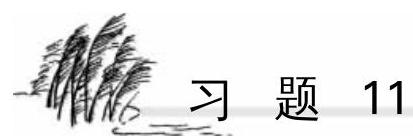
\includegraphics[max width=\textwidth, center]{2024_10_30_bd799899fef40368a068g-091}

1 用求根公式分解因式: $x^{2}-3 x+5$ ;\\
2 用求根公式分解因式: $x^{2}-2 x-7$ ;\\
3 用求根公式分解因式: $3 x^{2}-5 x-2$ ;\\
4 用求根公式分解因式: $2 x^{2}-5 x+1$ ;\\
$5 x^{2}+x y+y^{2}$ 是不是 $x^{7}+y^{7}+(x+y)^{7}$ 的因式?\\
6 分解因式: $x^{4}+4 x^{3}+2 x^{2}+x-2$.

这一单元介绍在有理数集内如何判定一个多项式是否既约.

\section*{12.1 艾氏判别法}
下面我们着重讨论一元的情形。\\
在复数集内,只有一次多项式是既约多项式。在实数集内,既约多项式是一次或二次多项式. 与这形成鲜明的对比的是,在有理数集内有任意次的既约多项式. 为了证明这一点, 先介绍一下重要的艾森斯坦(Eisenstein, 1823~ 1852)判别法:

设 $f(x)=a_{n} x^{n}+a_{n-1} x^{n-1}+\cdots+a_{1} x+a_{0}$ 是整系数多项式。\\
如果存在一个质数 $\boldsymbol{p}$ 满足以下条件:

\begin{enumerate}
  \item $p$ 不整除 $a_{n}$;
  \item $p$ 整除其余的系数 $\left(a_{0}, a_{1}, \cdots, a_{n-1}\right)$;
  \item $p^{2}$ 不整除 $a_{0}$ 。
\end{enumerate}

那么, $f(x)$ 在有理数集内不可约。\\
这个定理的证明在高等代数里可以找到, 我们就不赘述了(虽然证明并不困难)。

例1 证明:对于任意的自然数 $n, x^{n}-2$ 在有理数集内不可约.\\
证明 取 $p=2$, 则 $p$ 整除 $a_{0}=-2, p^{2}$ 不整除 $a_{0}, p$ 整除 $a_{1}=a_{2}=\cdots=$ $a_{n-1}=0$ ( 0 是任何一个非零整数的倍数), $p$ 不整除 $a_{n}=1$. 根据艾氏判别法, $x^{n}-2$ 是有理数集内的既约多项式。

例1已经表明在有理数集内存在着任意次的既约多项式.\\
例2 证明: $x^{4}+x^{3}+x^{2}+x+1$ 在有理数集内不可约。\\
证明 艾氏判别法不能直接应用。但令

\begin{align*}
x=y+1,
\end{align*}

则

\begin{align*}
x^{4}+x^{3}+x^{2}+x+1
\end{align*}

\begin{align*}
\begin{aligned}
& =\frac{x^{5}-1}{x-1} \\
& =\frac{(y+1)^{5}-1}{y} \\
& =y^{4}+5 y^{3}+10 y^{2}+10 y+5
\end{aligned}
\end{align*}

$y^{4}+5 y^{3}+10 y^{2}+10 y+5$ 中除首项系数 1 以外,其他系数都被 $p=5$ 整除,常数项 5 不能被 $p^{2}$ 整除。因此, $y^{4}+5 y^{3}+10 y^{2}+10 y+5$ 在有理数集内不能分解。从而 $x^{4}+x^{3}+x^{2}+x+1$ 也是有理数集内的既约多项式。

用这个方法可以证明,在 $p$ 为质数时,多项式 $x^{p-1}+x^{p-2}+\cdots+x+1$ 是有理数集内的既约多项式。

例3 证明: $x^{6}+x^{3}+1$ 在有理数集内不可约。\\
证明 令 $x=y+1$, 则

\begin{align*}
\begin{aligned}
& x^{6}+x^{3}+1 \\
= & (y+1)^{6}+(y+1)^{3}+1 \\
= & y^{6}+6 y^{5}+15 y^{4}+21 y^{3}+18 y^{2}+9 y+3 .
\end{aligned}
\end{align*}

由艾氏判别法(取 $p=3$ ) 可知这个多项式是既约多项式.

\section*{12.2 奇与偶}
如果把所有的奇数用 1 表示,偶数用 0 表示,那么就得到一种奇怪的算术:

\begin{align*}
0+0=0,0+1=1+0=1,1+1=0
\end{align*}

它们表示两个偶数的和是偶数;一个偶数与一个奇数的和是奇数;两个奇数的和是偶数。(在数论中,这是以 2 为模的算术)

采用这种算术,可以使问题大为简化,不但整数只有两个( 0 与 1 ),而且多项式的个数也大大减少。一次多项式只有两个,即

\begin{align*}
x, x+1
\end{align*}

实际上,如 $3 x+4$ 可以归为第一种, $3 x+5$ 可以归为第 2 种,而 $2 x+4=0$ 不是一次多项式. 二次多项式只有 4 个,即

\begin{align*}
x^{2}, x^{2}+x, x^{2}+1, x^{2}+x+1,
\end{align*}

其中, $x^{2}=x \cdot x, x^{2}+x=x(x+1), x^{2}+1=(x+1)^{2}$ ,都不是既约多项式,只有 $x^{2}+x+1$ 是既约多项式。

例4 证明:当 $(b+c) d$ 为奇数时,整系数的三次多项式 $x^{3}+b x^{2}+c x+$ $d$ 在有理数集内不可约。

证明 由于 $(b+c) d$ 是奇数,所以 $b+c$ 与 $d$ 都是奇数。如果 $x^{3}+b x^{2}+$ $c x+d$ 在有理数集内可以分解,那么它一定有一次因式,也就是有有理根,这根是整数而且是 $d$ 的约数,因而也是奇数。采用上面的算术,就有

\begin{align*}
b+c=1, d=1
\end{align*}

并且1是 $x^{3}+b x^{2}+c x+d$ 的根。但是

\begin{align*}
\begin{aligned}
& 1^{3}+b \cdot 1^{2}+c \cdot 1+d \\
= & 1+(b+c)+d \\
= & 1+1+1 \\
= & 1 \neq 0,
\end{aligned}
\end{align*}

所以, 1 不是 $x^{3}+b x^{2}+c x+d$ 的根,矛盾! 这说明当 $(b+c) d$ 为奇数时, $x^{3}+$ $b x^{2}+c x+d$ 在有理数集内不可约。

例 5 证明 $x^{5}+x^{2}-1$ 在有理数集内不可约。\\
证明 如果 $x^{5}+x^{2}-1$ 可以分解,那么它一定有一个一次因式或一个二次既约因式。

采用上面的算术,便得到 $x^{5}+x^{2}-1$ 应当被 $x 、 x+1$ 或 $x^{2}+x+1$ 中某一个整除。但

\begin{align*}
\begin{aligned}
& x^{5}+x^{2}-1 \\
= & x^{2}\left(x^{3}-1\right)+1 \\
= & x^{2}(x+1)\left(x^{2}+x+1\right)+1
\end{aligned}
\end{align*}

\begin{align*}
=x^{2}\left(x^{3}-1\right)+1 \quad[\text { 请注意 }+1 \text { 与 }-1 \text { 并无差别 }]
\end{align*}

可见, $x^{5}+x^{2}-1$ 不被 $x 、 x+1 、 x^{2}+x+1$ 中任一个整除。这就说明 $x^{5}+$ $x^{2}-1$ 在有理数集内不可约。

例 6 证明 $x^{6}+x^{3}-1$ 在有理数集内不可约。\\
证明 采用上面的算术,得

\begin{align*}
\begin{aligned}
& x^{6}+x^{3}-1 \\
= & \left(x^{6}-1\right)+\left(x^{3}-1\right)+1 \\
= & \left(x^{3}+2\right)\left(x^{3}-1\right)+1 \\
= & \left(x^{3}+2\right)(x-1)\left(x^{2}+x+1\right)+1 \\
= & x^{3}(x+1)\left(x^{2}+x+1\right)+1
\end{aligned}
\end{align*}

可见, $x^{6}+x^{3}-1$ 不被 $x 、 x+1 、 x^{2}+x+1$ 中任一个整除,故 $x^{6}+x^{3}-1$ 没有一次、二次的因式。

又因为由第 9 单元例 4 ,我们已经知道 $x^{6}+x^{3}-1$ 不能分解成三次因式的积,所以 $x^{6}+x^{3}-1$ 在有理数集内不可约。

例7 证明 $x^{4}+3 x^{3}+3 x^{2}-5$ 在有理数集内不可约。\\
证明 采用上面的算术,得

\begin{align*}
\begin{aligned}
& x^{4}+3 x^{3}+3 x^{2}-5 \\
= & x^{4}+x^{3}+x^{2}+1 \\
= & x^{3}(x+1)+\left(x^{2}+x\right)+(x+1) \\
= & (x+1)\left(x^{3}+x+1\right),
\end{aligned}
\end{align*}

因此,如果 $x^{4}+3 x^{3}+3 x^{2}-5$ 可以分解,它一定分解为一个一次因式与一个三次因式的积。

容易验证, $x^{4}+3 x^{3}+3 x^{2}-5$ 没有有理根,自然它就没有一次因式,从而它在有理数集内不可约。

\section*{12.3 分圆多项式}
在第 11 单元例 11 ,我们获得了 $x^{15}-1$ 的分解式:\\
$x^{15}-1$\\
$=(x-1)\left(x^{2}+x+1\right)\left(x^{4}+x^{3}+x^{2}+x+1\right)\left(x^{8}-x^{7}+x^{5}-x^{4}+x^{3}-x+1\right)$.\\
这是 1978 年全国数学联赛的一道赛题. 后来又被一位教授用作对研究生的考题。

为什么一道中学生的赛题可以作为研究生的考题呢?原来这道题的分解并不太难,可是,要证明 $x^{4}+x^{3}+x^{2}+x+1$ 与 $x^{8}-x^{7}+x^{5}-x^{4}+x^{3}-x+1$都是在有理数集内既约多项式却不容易。前一个式子在有理数集内的既约性,我们已在例 2 中予以证明了。现在,我们用初等的方法来证明后一个式子在有理数集内的既约性。

例8 证明 $x^{8}-x^{7}+x^{5}-x^{4}+x^{3}-x+1$ 在有理数集内是既约多项式。\\
证明 采用前面所说的以 2 为模的算术,这时

\begin{align*}
\begin{align*}
& x^{8}-x^{7}+x^{5}-x^{4}+x^{3}-x+1 \\
= & \left(x^{8}+x^{5}+x^{4}\right)+\left(x^{7}+x^{4}+x^{3}\right)+\left(x^{4}+x+1\right) \\
= & \left(x^{4}+x+1\right)\left(x^{4}+x^{3}+1\right) .
\end{align*} \tag{1}
\end{align*}

$x^{4}+x+1$ 与 $x^{4}+x^{3}+1$ 都是既约多项式。因此,如果 $x^{8}-x^{7}+x^{5}-x^{4}+$ $x^{3}-x+1$ 在有理数集内可以分解,那么它必定分解为两个四次既约因式

的积。\\
下面证明 $x^{8}-x^{7}+x^{5}-x^{4}+x^{3}-x+1$ 在有理数集内不可能有四次既约因式。实际上,设 $x^{4}+a x^{3}+b x^{2}+c x+d$ 是它的四次既约因式,其中 $a 、 b 、 c 、 d$为整数。由于 $x^{8}-x^{7}+x^{5}-x^{4}+x^{3}-x+1$ 的根都是虚单位根(15次单位根), $x^{4}+a x^{3}+b x^{2}+c x+d$ 的根也是虚单位根,并且两两共轭。其中一对共轭因式的积为

\begin{align*}
\begin{aligned}
& {\left[x-\left(\cos \frac{2 m \pi}{15}+i \sin \frac{2 m \pi}{15}\right)\right]\left[x-\left(\cos \frac{2 m \pi}{15}-i \sin \frac{2 m \pi}{15}\right)\right] } \\
= & x^{2}-\left(2 \cos \frac{2 m \pi}{15}\right) x+1
\end{aligned}
\end{align*}

同理,另一对共轭因式的积为

\begin{align*}
\begin{aligned}
& {\left[x-\left(\cos \frac{2 n \pi}{15}+i \sin \frac{2 n \pi}{15}\right)\right]\left[x-\left(\cos \frac{2 n \pi}{15}-i \sin \frac{2 n \pi}{15}\right)\right] } \\
= & x^{2}-\left(2 \cos \frac{2 n \pi}{15}\right) x+1
\end{aligned}
\end{align*}

这两式中 $m 、 n$ 为 $1 \sim 7$ 中的整数,且 $m \neq n$ 。\\
因而两对共轭因式的积为

\begin{align*}
\begin{aligned}
& {\left[x^{2}-\left(2 \cos \frac{2 m \pi}{15}\right) x+1\right]\left[x^{2}-\left(2 \cos \frac{2 n \pi}{15}\right) x+1\right] } \\
= & x^{4}-\left(2 \cos \frac{2 m \pi}{15}+2 \cos \frac{2 n \pi}{15}\right) x^{3}+\cdots-\left(2 \cos \frac{2 m \pi}{15}+2 \cos \frac{2 n \pi}{15}\right) x+1,
\end{aligned}
\end{align*}

即 $x^{4}+a x^{3}+b x^{2}+c x+d$ 中的系数 $a=c$ 。\\
但是,由(1)式可知,在四次因式中, $x^{3}$ 与 $x$ 的系数是不同的(奇偶性不同),因此 $x^{8}-x^{7}+x^{5}-x^{4}+x^{3}-x+1$ 没有四次既约因式,它本身是有理数集内的既约多项式。

实际上, $x^{8}-x^{7}+x^{5}-x^{4}+x^{3}-x+1$ 是分圆多项式,它的根都是 15 次本原单位根. 在代数中有一条更一般的定理:

分圆多项式在有理数集内是不可约的。\\
例如:多项式 $x^{4}+1=\frac{x^{8}-1}{x^{4}-1}$ ,它的根是 8 次本原单位根;例 3 中的 $x^{6}+$ $x^{3}+1=\frac{x^{9}-1}{x^{3}-1}$, 它的根是 9 次本原单位根; 例 2 中的 $x^{4}+x^{3}+x^{2}+x+1=$ $\frac{x^{5}-1}{x-1}$ ,它的根是 5 次本原单位根. 这些多项式都是分圆多项式,在有理数集内都是不可约的.

\section*{12.4 绝对不可约}
多元多项式的既约问题更为复杂. 有些多项式在有理数集内不可约,但在数集扩大后却可以分解。例如 $y^{2}-2 x^{2}$ 在有理数集内不可约,在实数集内,有

\begin{align*}
\begin{aligned}
& y^{2}-2 x^{2} \\
= & (y+\sqrt{2} x)(y-\sqrt{2} x) .
\end{aligned}
\end{align*}

又如 $x^{2}+2 x+1+y^{2}$ 在实数集与有理数集内均不可约. 在复数集内, 有

\begin{align*}
\begin{aligned}
& x^{2}+2 x+1+y^{2} \\
= & (x+1+\mathrm{i} y)(x+1-\mathrm{i} y) .
\end{aligned}
\end{align*}

也有些多元多项式,即使在复数集内也不能分解,这样的多项式称为绝对不可约的。例如二元二次多项式 $a x^{2}+b x y+c y^{2}+d x+e y+f$ 在

\begin{align*}
4 a c f+b e d-c d^{2}-a e^{2}-f b^{2} \neq 0
\end{align*}

时,绝对不可约(在解析几何中可以知道,这也就是二次曲面 $a x^{2}+b x y+$ $c y^{2}+d x+e y+f=0$ 不退化为两条直线的充分必要条件). 在

\begin{align*}
4 a c f+b e d-c d^{2}-a e^{2}-f b^{2}=0 \tag{2}
\end{align*}

时,这个多项式在复数集内可以分解为两个一次因式的积。当 $b^{2}-4 a c \geqslant 0$ , $d^{2}-4 a f \geqslant 0, e^{2}-4 c f \geqslant 0$ 同时成立时,这个多项式在实数集内也可以分解。如果还有条件: $b^{2}-4 a c, d^{2}-4 a f, e^{2}-4 c f$ 都是有理数的平方,那么这个多项式在有理数集内可以分解。

小 结\\
在有理数集内,存在着任意次的既约多项式。可以利用艾森斯坦判别法、奇偶性(以 2 为模的算术)及待定系数法等来证明多项式是既约多项式。\\
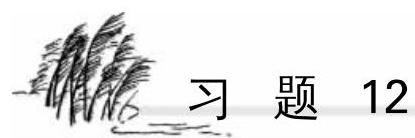
\includegraphics[max width=\textwidth, center]{2024_10_30_bd799899fef40368a068g-097}

证明以下各式在有理数集内不可约:\\
$1 x^{4}+x+1$.\\
$2 x^{4}+x^{3}+1$.\\
$3 x^{6}-x^{3}-1$.\\
$4 x^{4}+5 x+21$.\\
$5 x^{4}+x^{3}+12 x^{2}+14 x+1$.

\section*{习 题 1}
\begin{enumerate}
  \item $5 x y(x-2 z+1)$
  \item $(x-a)(a-b-1)$
  \item $(x+1)(a+1-2 x)$
  \item $\frac{1}{6} b^{2 n-1}\left(9 b^{n}+1\right)$
  \item $2(p-1)(p-1-2 q)$
  \item $n(m-n)\left(m^{2}+n^{2}\right)$
  \item $(2 m+3 p)(3 a+5 b)$
  \item $2(x+y)\left(1+3 x+3 y-2 x^{2}-4 x y-2 y^{2}\right)$
  \item $(x+y)(b+c)(x+y-b-c)$
  \item $2 p(x-1)^{2}(3 x-4 p-4)$
\end{enumerate}

\section*{习 题 2}
\begin{enumerate}
  \item $(4+3 a+2 b)(4-3 a-2 b)$
  \item $(2 y+2 z-x)(2 y-2 z+x)$
  \item $(a+b)(a-b)\left(a^{2}+b^{2}\right)$
  \item $(2 c+3 a b)(2 c-3 a b)\left(4 c^{2}+9 a^{2} b^{2}\right)$
  \item $5 a x(2 a x+3 y)(2 a x-3 y)$
  \item $8(a+b)(a-b)\left(a^{2}+b^{2}\right)$
  \item $(x-y)(x+y)\left(x^{2}+y^{2}\right)\left(x^{4}+y^{4}\right)$
  \item $x(2 x-1)(2 x+1)\left(4 x^{2}+1\right)$
  \item $24 x(x-1)(x+1)^{2}$
  \item $4 b^{3}\left(2 a-b^{2}\right)\left(4 a^{2}+2 a b^{2}+b^{4}\right)$
  \item $(2 a b c-1)\left(4 a^{2} b^{2} c^{2}+2 a b c+1\right)$
  \item $y^{3}\left(4 x^{2}+y^{4}\right)\left(16 x^{4}-4 x^{2} y^{4}+y^{8}\right)$
  \item $(a x+b x-a y+b y)^{2}$
  \item $a^{n-2}\left(a^{2}+4\right)^{2}$
  \item $\left(3 a+x^{n}+1\right)^{2}$
  \item $(a+b-c)^{2}$
  \item $(x-3 y+2 z)^{2}$
  \item $8 q^{3}$
  \item $-(a+b)^{2}(a-b)^{2}$
  \item $8 a x\left(a^{2}+x^{2}\right)$
\end{enumerate}

\section*{习 题 3}
\begin{enumerate}
  \item $(x-y)(a+b-c)$
  \item $(x+1)\left(x^{3}+x-1\right)$
  \item $\left(1-b+b^{2}\right)(a-1)$
  \item $\left(a^{2}+x^{2}\right)(4 x-1)$
  \item $(b x-y)(a x+y)$
  \item $(a b+c d)\left(a b^{2}-c^{2} d\right)$
  \item $\left(2 c^{2}-3 x^{2}\right)(16 a-5 c)$
  \item $(x+2 a)(2 x-3 b)$
  \item $(x+y)\left(x^{2}-x y+y^{2}-1\right)$
  \item $(x+y)\left(x^{2}-x y+y^{2}+x+y\right)$
  \item $(2 a+c+b-3 d)(2 a+c-b+3 d)$
  \item $(1-b)^{2}(a-1)$
  \item $(x-y)(x+y+z)$
  \item $(x+b)\left(x^{2}+a\right)$
  \item $(a x+b)\left(c x^{2}+d\right)$
  \item $(a+b)(a-b)\left(a^{2}+a b+b^{2}\right)$
  \item $(a-b)^{2}\left(a^{2}+a b+b^{2}\right)$
  \item $(a+1)(a-1)(b+1)(b-1)$
  \item $(x+z)(x-z)(y+z)(y-z)$
  \item $\left(y^{2} z-1\right)\left(x^{2} z-1\right)$
  \item $(x+y)(x+z)\left(x^{2}-x z+z^{2}\right)$
  \item $2(a+b+c+d)(a-d)$
  \item $\left(b^{2} x+a y^{2}\right)(x y+a b)$
  \item $3(a+b+c)\left(a^{2}+b^{2}+c^{2}\right)$
\end{enumerate}

\section*{习 题 4}
\begin{enumerate}
  \item $\left(x^{2}+x-1\right)\left(x^{2}-x-1\right)$
  \item $\left(x^{2}+5 x y+9 y^{2}\right)\left(x^{2}-5 x y+9 y^{2}\right)$
  \item $\left(x^{2}+5 x+1\right)\left(x^{2}-5 x+1\right)$
  \item $\left(x^{2}+4 x y+y^{2}\right)\left(x^{2}-4 x y+y^{2}\right)$
  \item $\left(x^{2}-x+1\right)\left(x^{2}+x+1\right)\left(x^{4}-x^{2}+1\right)$
  \item $\left(x^{2}+7 x+1\right)\left(x^{2}-7 x+1\right)$
  \item $\left(x^{6}+x^{3}-1\right)\left(x^{6}-x^{3}-1\right)$
  \item $\left(x^{2}-x y+y^{2}\right)(a x+b y+x+y)$
  \item $(x+y-2)(x-y+4)$
  \item $\left(x^{2}+4 x+8\right)\left(x^{2}-4 x+8\right)$
  \item $(1-a x)\left(1-a x-c x^{2}\right)$
  \item $(x-y)^{2}(2 x-z)$
\end{enumerate}

\section*{习 题 5}
\begin{enumerate}
  \item $(x+2)(x+10)$
  \item $(x-2)(x-10)$
  \item $(x+1)(x-5)$
  \item $(x-11)(x+2)$
  \item $(4 x+3 y)(3 x-5 y)$
  \item $(2 x-3)(3 x-2)$
  \item $(x+3)(2 x+1)$
  \item $(2 x-3)(x-1)$
  \item $(x-4 y)(x-16 y)$
  \item $-(x+7)(x-8)$
\end{enumerate}

\section*{习 题 6}
\begin{enumerate}
  \item $(x+y+1)(x+y+2)$
  \item $(4 x-2 y+1)(x-3 y-2)$
  \item $(x+y-3 z)(x-y+z)$
  \item $(x-2 y-a)(2 x-y+a)$
  \item $(a+b-3 c)(a-3 b+c)$
  \item $(a+2 b-3)(2 a-11 b+1)$
  \item $(x-y+3 z)(x+2 y-z)$
  \item $(x-2 y+3 z)(2 x+3 y+z)$
  \item $(2 x+3 y+2 z)(2 x-3 y+z)$
  \item $(x+2 z)(4 x+y+z)$
\end{enumerate}

\section*{习 题 7}
\begin{enumerate}
  \item $(x-y)(x+y)(x-3 y)(x+3 y)$
  \item $(x+2 y)(x-3 y)\left(x^{2}-2 x y+4 y^{2}\right)\left(x^{2}+3 x y+9 y^{2}\right)$
  \item $(x+a+b)(x-a-b)(x+a-b)(x-a+b)$
  \item $(a+b)^{2}(a-b)^{2}(x+y)^{2}(x-y)^{2}$
  \item $\left(a^{2}+a b+b^{2}\right)\left(x^{2}+x y+y^{2}\right)$
  \item $(x+1)(x-1)(x-x y+1+y)(x-x y-1-y)$
  \item $(a b x+c)(c x+a b)$
  \item $(x+1)(a x-b x+a+b)$
  \item $(x+a+b)(x+c)$
  \item $(a b+c+d)(a c-d)$
  \item $(x+1)(x-1)(x+a)(x-a)$
  \item $\left(x^{2}+x+1+a\right)\left(x^{2}-x+1-a\right)$
  \item $3 a b x y(a+b)(x+y)$
  \item $(x+2)(x+6)\left(x^{2}+8 x+10\right)$
  \item $a(a-5)\left(a^{2}-5 a+10\right)$
  \item $(x-1)(x+2)\left(x^{2}+x+6\right)$
  \item $\left(x^{2}+6 x+4\right)(x+2)^{2}$
  \item $9(x+1)^{2}\left(x^{2}+4 x+1\right)$
  \item $(x+2)(x-1)(x-3)(x+4)$
  \item $(x+2)(x+4)\left(x^{2}+5 x+8\right)$
  \item $(x-1)(x+2)\left(x^{2}+x+5\right)$
  \item $\left(x^{2}+10 x+18\right)\left(x^{2}+10 x+22\right)$
\end{enumerate}

\section*{习 题 8}
\begin{enumerate}
  \item $(x-1)\left(x^{2}+5 x+5\right)$
  \item $(x+1)^{3}\left(2 x^{2}+x+3\right)$
  \item $(x+y)(x-y)^{3}$
  \item $(x-1)^{2}(x+2)^{2}$
  \item $(x+1)(2 x-1)\left(x^{2}+4\right)$
  \item $(x-y)^{2}(3 x+y)$
  \item $(x-y)(2 x-y)(3 x+2 y)$
  \item $(x+2)\left(3 x^{2}+4\right)$
  \item $(2 x+a)(2 x+b)(2 x+c)$
  \item $(x-1)^{2}(a x-x+a-2)$
  \item $(5 x+7)\left(x^{3}+x^{2}+2 x-1\right)$
  \item $(x+p-1)\left(x^{2}+x+1\right)$
\end{enumerate}

\section*{习 题 9}
\begin{enumerate}
  \item $\left(2 x^{2}-x-2\right)\left(x^{2}+2 x-1\right)$
  \item $\left(x^{2}-x-1\right)\left(x^{2}+x+2\right)$
  \item $\left(x^{2}-x+1\right)\left(2 x^{2}+x+1\right)$
  \item 不能
  \item 不能
\end{enumerate}

\section*{习 题 10}
\begin{enumerate}
  \item $-(a-b)(b-c)(c-a)$
  \item $(a+b)(b+c)(c+a)$
  \item $(a-b)(a-c)(b+c)$ (上题的 $a$ 换为 $-a)$
  \item $(a-b)(b-c)(c-a)$
  \item $3(x+y)(y+z)(z+x)$
  \item $-(a-b)(b-c)(c-a)$
  \item $-4(a-b)(b-c)(c-a)$
  \item $(x+y)(y+z)(z+x)$
  \item $2 a b c$
  \item $4 a b c$
  \item $4 a b c$
  \item $(a+b)(b+c)(c+a)$
  \item $(a+b+c)\left(a^{2}+b^{2}+c^{2}\right)$
  \item $-3(a-b)(b-c)(c-a)$
  \item $(a+b-1)\left(a^{2}+b^{2}-a b+a+b+1\right)$
  \item $\left(x^{2}-3 y+3\right)\left(x^{4}+9 y^{2}+3 x^{2} y+9 y+3\right)$
  \item $3 a b c(b z-c y)(c x-a z)(a y-b x)$
  \item $(a+b+c)(a-b)(b-c)(c-a)$
  \item $-2(a-b)(b-c)(c-a)(a+b+c)$
  \item $(a+b)(b+c)(c+a)(a+b+c)$
  \item $-(a-b)(b-c)(c-a)\left(a^{2}+b^{2}+c^{2}+a b+b c+c a\right)$
  \item $-(a-b)(b-c)(c-a)(a b+b c+c a)$
  \item $(a-b)(b-c)(c-a)\left(a^{2}+b^{2}+c^{2}+a b+b c+c a\right)$
  \item $5 a b(a+b)\left(a^{2}+a b+b^{2}\right)$
  \item $5(x+y)(y+z)(z+x)\left(x^{2}+y^{2}+z^{2}+x y+y z+z x\right)$
  \item $80 a b c\left(a^{2}+b^{2}+c^{2}\right)$
  \item $(x-y)(y-z)(z-x)(x y+y z+z x)$
  \item $-(a-b)(b-c)(c-a)\left(3 a^{2}+3 b^{2}+3 c^{2}+5 a b+5 b c+5 c a\right)$
  \item $-(a-b)(b-c)(c-a)(a+b+c)^{2}$
  \item $2 a b c(a b+b c+c a)$
  \item $-(b-c)(b+c)(c-a)(c+a)(a-b)(a+b)$
  \item $-(a-b)(b-c)(c-a)\left(a^{3}+b^{3}+c^{3}+a^{2} b+b^{2} c+c^{2} a+a b^{2}+b c^{2}+a^{2}+\right.$ $a b c)$
  \item $(a-b)(b-c)(c-a)\left(a^{3}+b^{3}+c^{3}+a^{2} b+b^{2} c+c^{2} a+a b^{2}+b c^{2}+\right.$ $\left.c a^{2}-9 a b c\right)$
  \item $27 a^{2} b^{2}(a+b)^{2}$
  \item $-7 x y(x+y)\left(x^{2}+x y+y^{2}\right)^{2}$
  \item $-(a-b)(b-c)(c-a)\left(a^{2} b^{2}+b^{2} c^{2}+c^{2} a^{2}+a^{2} b c+b^{2} c a+c^{2} a b\right)$
  \item $(x-y)\left(x^{2}+x y+y^{2}\right)(y-z)\left(y^{2}+y z+z^{2}\right)(z-x)\left(z^{2}+z x+x^{2}\right)$
  \item $(a-b)(b-c)(c-a)(a-d)(b-d)(c-d)$
\end{enumerate}

\section*{习 题 11}
\begin{enumerate}
  \item $\left(x-\frac{3+\sqrt{11} \mathrm{i}}{2}\right)\left(x-\frac{3-\sqrt{11} \mathrm{i}}{2}\right)$
  \item $(x-1+2 \sqrt{2})(x-1-2 \sqrt{2})$
  \item $(3 x+1)(x-2)$
  \item $2\left(x-\frac{5+\sqrt{17}}{4}\right)\left(x-\frac{5-\sqrt{17}}{4}\right)$
  \item 是
  \item $\left(x^{2}+x+1\right)\left(x^{2}+3 x-2\right)$
\end{enumerate}

\section*{习 题 12}
\begin{enumerate}
  \item 在以 2 为模的算术中, $x^{4}+x+1=x(x+1)\left(x^{2}+x+1\right)+1$ 不被一次与二次既约因式 $x 、 x+1 、 x^{2}+x+1$ 整除
  \item 若依升幂排列与上题实质是一样的
  \item 同例6证明(利用习题 9 第 5 题)
  \item 在以 2 为模的算术中,同 $x^{2}+x+1$
  \item 在以 2 为模的算术中,同 $x^{4}+x^{3}+1$
\end{enumerate}


\end{document}